 \chapter{Sviluppo dell'applicazione}
In questo capitolo verranno trattati gli argomenti relativi alla progettazione e allo sviluppo concreto dell'applicazione. Si procederà con l'introduzione dei \textit{requisiti} che l'applicazione deve soddisfare, per poi esporre le scelte progettuali e le motivazioni che hanno portato alla realizzazione dell'architettura finale. Le varie architetture verranno introdotte prima da un punto di vista teorico, per poi affrontare una spiegazione più tecnica, strettamente legata all'effettiva implementazione.

\section{Requisiti}
L'applicazione deve essere in grado di interrogare un server tramite una \textit{socket}, la quale invierà come risposta il set di dati, rilevati dai sensori installati sulla barca. L'applicazione deve svolgere un \textit{polling} della socket, periodicamente per un tempo prefissato. Questi dati dovranno essere organizzati e visualizzati su più schermate, in modo da facilitare l'utente nel monitorare i dati di cui necessita.

Rispetto all'applicazione Android sviluppata precedentemente, si vuole ridisegnare l'interfaccia grafica in modo da rendere la visualizzazione dei dati il più efficace possibile.

Si vuole inoltre disporre di alcune funzionalità come la possibilità che l'utente possa decidere ogni quanti secondi interrogare il server e che questo non sia un parametro fisso integrato nel codice.

In conclusione, si vuole rendere l'applicazione disponibile sia per gli utenti con dispositivi Android che iOS. Pertanto la scelta di un framework cross-platform risulta essere adatta nel rispettare questa particolare richiesta.

\section{Architetture utilizzate}

\subsection{Introduzione}
L'architettura rappresenta l'elemento fondante di tutta l'applicazione. Essa permette di definire le logiche e i comportamenti che avrà l'applicazione al termine dello sviluppo e definisce anche in che modo deve avvenire la cooperazione tra i vari componenti dell'applicazione. Un altro fattore importante da tenere in considerazione è il contesto in cui l'applicazione verrà utilizzata. Quindi, è necessario quindi scegliere attentamente l'architettura corretta sulla base dei requisiti e del risultato finale che si vuole ottenere. Il processo di scelta dell'architettura richiede una certa esperienza nella programmazione, nel conoscere il framework con il quale si creerà l'applicazione ed una conoscenza delle nozioni di \textit{ingegneria del software}.

Nella scelta dell'architettura influiscono anche proprietà come le \textit{prestazioni} che si vogliono ottenere e la \textit{flessibilità} dell'architettura stessa, necessaria per poter supportare l'implementazione di nuove funzionalità in futuro.

In conclusione, la scelta dell'architettura è una fase particolarmente delicata ed importante in quanto determinerà il successo nel raggiungere i requisiti richiesti o il mancato raggiungimento di essi.

\subsection{Scelta dell'architettura}
L'architettura scelta farà un largo uso della \textit{programmazione reattiva}, caratteristica peculiare del linguaggio del framework.

Un principale svantaggio dell'utilizzo di Flutter come framework di sviluppo è il suo recente rilascio nel mercato. Essendo un framework relativamente nuovo rispetto agli altri, la comunità di Flutter ha proposto diverse architetture e pattern per implementare le applicazioni. Tuttavia, Google non ha mai fornito un supporto alla realizzazione di un qualche pattern ideale nelle sue guide relative al framework. Nella sua documentazione, il team di Flutter ha soltanto racchiuso in una pagina una serie di link alle risorse che illustrano alcuni pattern, spiegati da chi li hanno ideati. Pertanto, la ricerca e l'analisi di dell'architettura adatta è un processo più laborioso rispetto ad altri framework già affermati nel mercato.

\newpage

\subsection{Provider}
L'introduzione di questo pattern è di fondamentale importanza in quanto rappresenta il fulcro di tutto il pattern architetturale finale dell'applicazione. 

Una delle possibili definizioni per il pattern \textbf{Provider} può essere la seguente: \textit{"Il pattern Provider condivide i valori tra Widget tree e i Widget facenti parte dell'albero vengono ricostruiti in base ai cambiamenti di stato avvenuti nell'applicazione"}. Esaminando questa definizione è possibile affermare che:
\begin{enumerate}
	\item Il Provider è un Widget;
	\item Le dipendenze di un Provider sono dei Widget tree;
	\item Il Provider si occupa di aggiornare i Widget nel momento in cui rileva un cambiamento di stato;
\end{enumerate}

Da queste considerazioni, si può capire che l'aggiornamento debba avvenire in modo \textit{asincrono} e debba essere \textit{reattivo}. In particolare, i Widget che non cambiano con la generazione di un nuovo stato, non necessitano di dover rimanere in ascolto di un nuovo stato; i Widget che cambiano nel momento in cui viene rilevata una variazione dello stato dell'applicazione, devono rimanere in ascolto non appena un nuovo stato viene creato. Pertanto, in quest'ultima casistica, verranno utilizzati \verb|Future| e \verb|Stream|. 

Quando lo stato cambia, questo viene fornito al Provider piuttosto che a ciascun discendente (Widget). Per fare ciò il Provider utilizza internamente un \verb|InheritedWidget|, un oggetto che permette di propagare, in modo efficiente, i cambiamenti lungo il Widget tree. La gestione dell'aggiornamento dei Widget tree rappresenta uno dei principali problemi dello sviluppo dell'applicazione, in quanto questo fattore può essere uno dei principali responsabili del degrado delle prestazioni.

Il Provider rappresenta, sostanzialmente, un mezzo per condividere un valore per i Widget che ne necessitano. Con le successive spiegazioni, si andrà ad apprezzare la \textit{flessibilità} di questo pattern.

\subsubsection{Strutturazione del Provider}
Ricordando che questo pattern è un Widget e pertanto si inserirà nel Widget tree complessivo dell'applicazione, ogni Provider ha un \textit{figlio} (il parametro \verb|child|) che rappresenta la radice di un certo Widget tree (sottoalbero del Widget tree dell'app). Il Provider rende il valore disponibile per tutti i Widget a loro sottostanti. Ogni Widget decide individualmente se utilizzare o meno il valore ricevuto.

Non ci sono restrizioni su ciò che può essere un \textit{valore}. Può essere un \textit{servizio} (ad esempio un API), un \textit{modello} o uno \textit{stato}. Un modello potrebbe essere un oggetto che rappresenta una certa entità, come ad esempio un messaggio o un utente. Uno stato potrebbe essere il valore di un campo, la quantità di dati finora caricati o lo stato di riproduzione di un flusso di dati audiovisivo.

La scelta di non prendere i nuovi valori da delle variabili globali visibili a tutti i Widget che ne necessitano, è dovuta alla rigida gerarchia dei Widget tree, la quale impedisce che si verifichino delle \textit{dipendenze circolari}. Un'altra ragione, riguarda il passaggio di un valore attraverso più costruttori per farlo raggiungere ad uno specifico Widget dell'albero. Questa tecnica rende il codice complesso e verboso, pertanto vengono utilizzate le tecniche di \textit{dependency injection}.

Il Provider viene creato prima di istanziare tutti i Widget dipendenti che esso contiene (Figura 6.2). Costruire per primo il Provider, permette di avere già a disposizione dei valori per i Widget discendenti che \textbf{non sono ancora stati costruiti}. Quando i Widget dipendenti vengono successivamente creati, essi hanno accesso a tali valori e possono effettuare le loro modifiche grafiche in base ai valori ricevuti.

\subsubsection{Recuperare ed utilizzare i valori dal Provider}
\begin{figure}
	\begin{center}
		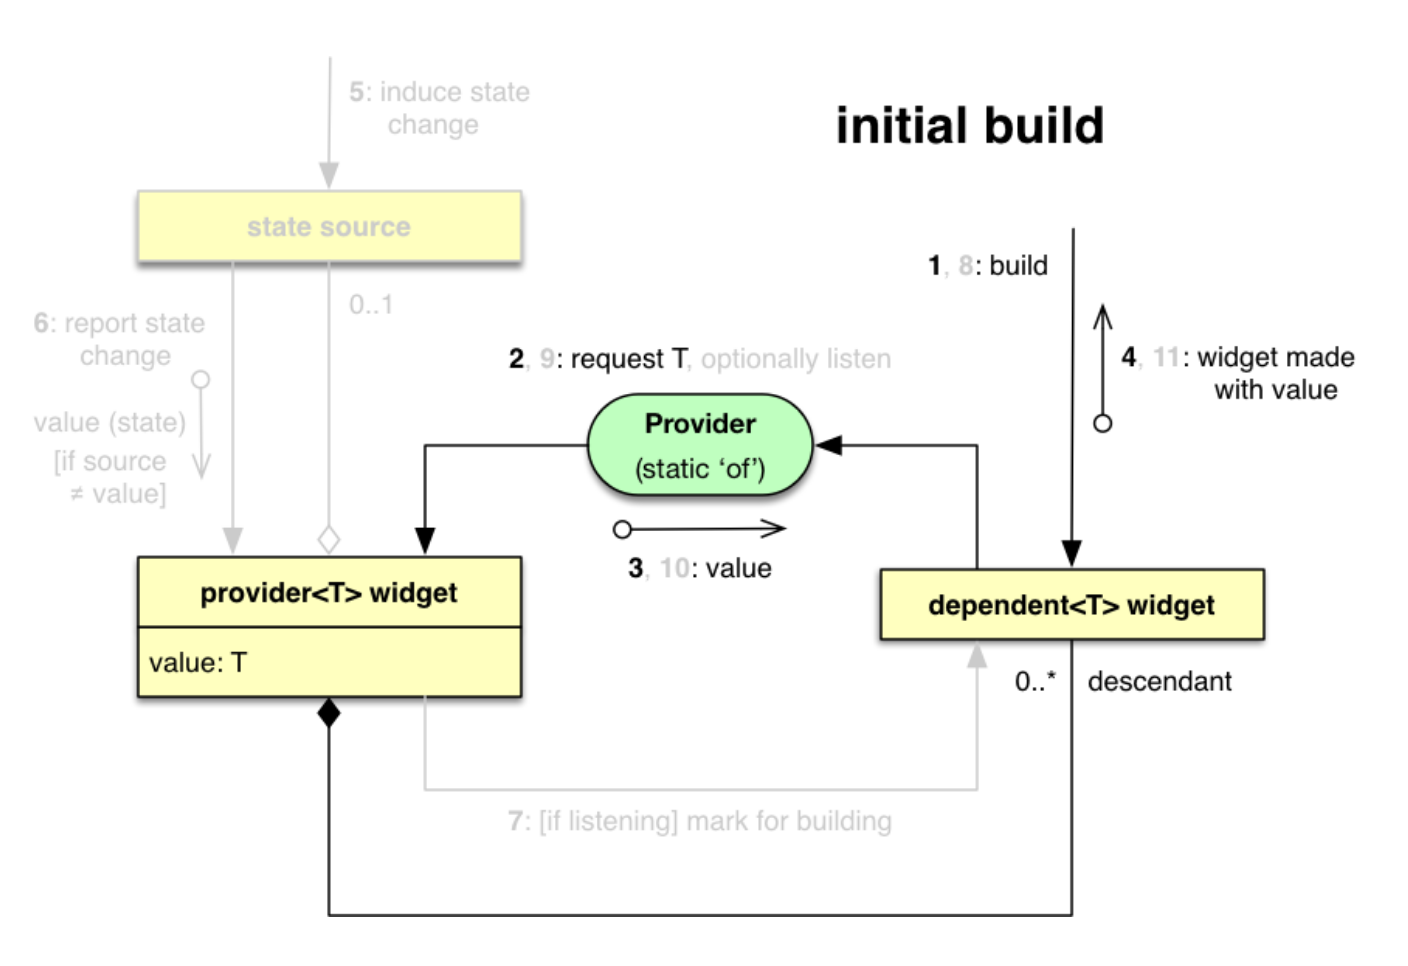
\includegraphics[scale=0.5]{provider_2}
		\caption[Provider - Inizializzazione]{Inizializzazione del Provider \cite{provider_first}.}
		\label{figura:provider_2}
	\end{center}
\end{figure}

I Widget possono riferirsi ai valori contenuti nel Provider con il metodo statico \verb|Provider.of<T>(context)|. Sulla base di questo metodo è possibile individuare un principale svantaggio di questo pattern: per poter recuperare i valori all'interno del Provider, è necessario che il metodo venga chiamato all'interno di un Widget (solitamente all'interno del metodo \verb|build()|) o che comunque gli venga passato un \verb|BuildContext context|. Questo svantaggio rappresenta una restrizione in quanto non è possibile utilizzare il Provider in classi dove non vi sia un \textit{contesto}. Ad esempio, il Provider non può essere utilizzato nelle classi che vanno a costituire la business logic.

Quando si va a definire e ad utilizzare un Provider, è necessario specificare il tipo di dato che il Provider deve rendere disponibile ai sui Widget discendenti. Questo significa che il Provider è una classe \textit{parametrica}: questo gli garantisce una certa flessibilità d'uso. Pertanto un Provider può rendere disponibile un valore di un qualsiasi tipo di dato.

Di seguito si introducono i passi che vengono svolti per poter istanziare il pattern:
\begin{enumerate}
	\item Come prima cosa Flutter si occupa della creazione del Provider. La costruzione del Provider implica la costruzione del figlio (\verb|child|) e la costruzione del figlio implica a sua volta la costruzione di tutti i Widget in esso contenuti. Il framework chiama il metodo \verb|build()| sul figlio per costruire il Widget che deve essere renderizzato. Questo metodo viene chiamato per tutti i Widget discendenti;
	\item Durante la compilazione (in particolare alla prima invocazione del metodo \verb|build()|), uno o più Widget discendenti, effettuano una chiamata al metodo \verb|Provider.of <T>()| per richiedere un valore. Questa chiamata viene fatta immediatamente dai Widget sottostanti, in quanto non possono essere creati senza un valore iniziale dello stato;
	\item Dopo che l'albero dei Widget è stato creato per la prima volta sulla base di uno stato iniziale, il Provider è in grado di ricevere i cambiamenti di stato. Al momento della ricostruzione dei Widget, il Provider crea un nuovo \verb|InheritedWidget| dalla stessa istanza del figlio utilizzata inizialmente. \verb|InheritedWidget| identifica i \textit{child} che stanno ascoltando i cambiamenti di stato e contrassegna soltanto i Widget che devono essere ricostruiti (Figura 6.2).
\end{enumerate}

\begin{figure}
	\begin{center}
		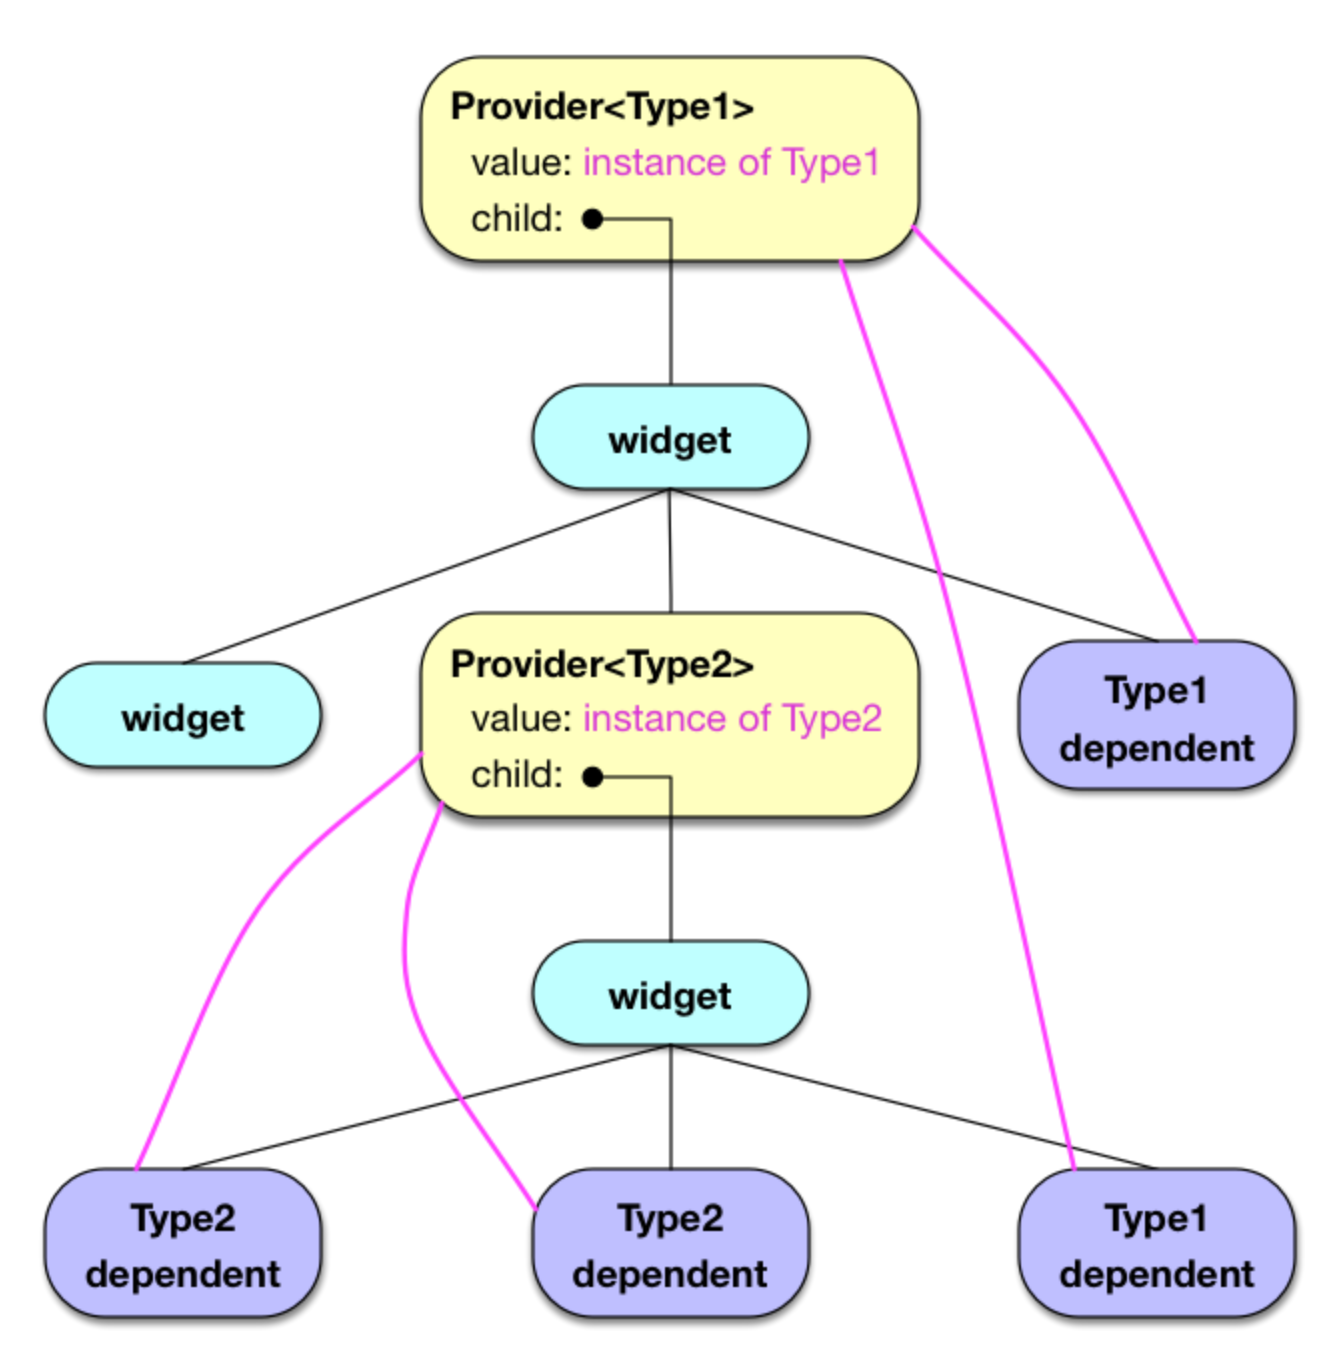
\includegraphics[scale=0.3]{provider_3}
		\caption[Provider - Aggiornamento]{Aggiornamento dei Widget a fronte di un cambiamento di stato \cite{provider_first}. Si può notare che non tutti i Widget vengono aggiornati ma soltanto quelli che hanno come "genitore" \textit{Provider.of \textless T \textgreater (context)}.}
		\label{figura:provider_3}
	\end{center}
\end{figure}

\label{consumer}
Nel momento in cui il Provider riceve un nuovo dato e lo deve rendere disponibile ai suoi discendenti, esso causerebbe il rendering di tutti i Widget sottostanti, anche di quelli che non sono influenzati dal cambiamento di stato. Pertanto, per ovviare a questa problematica, si può specificare esplicitamente quali Widget devono rimanere in ascolto per poter essere aggiornati di un nuovo cambiamento di stato (Figura 6.3). Ci sono vari modi per specificarlo:
\begin{enumerate}
	\item Chiamando il metodo \verb|Provider.of<T>(context)|;
	\item Utilizzando l'oggetto \verb|Consumer|
	\begin{lstlisting}
	Consumer<T>(
  		builder: (context, user, child) {
    			// Return a Widget tree
		}
	)
	\end{lstlisting}
\end{enumerate}

\begin{figure}
	\begin{center}
		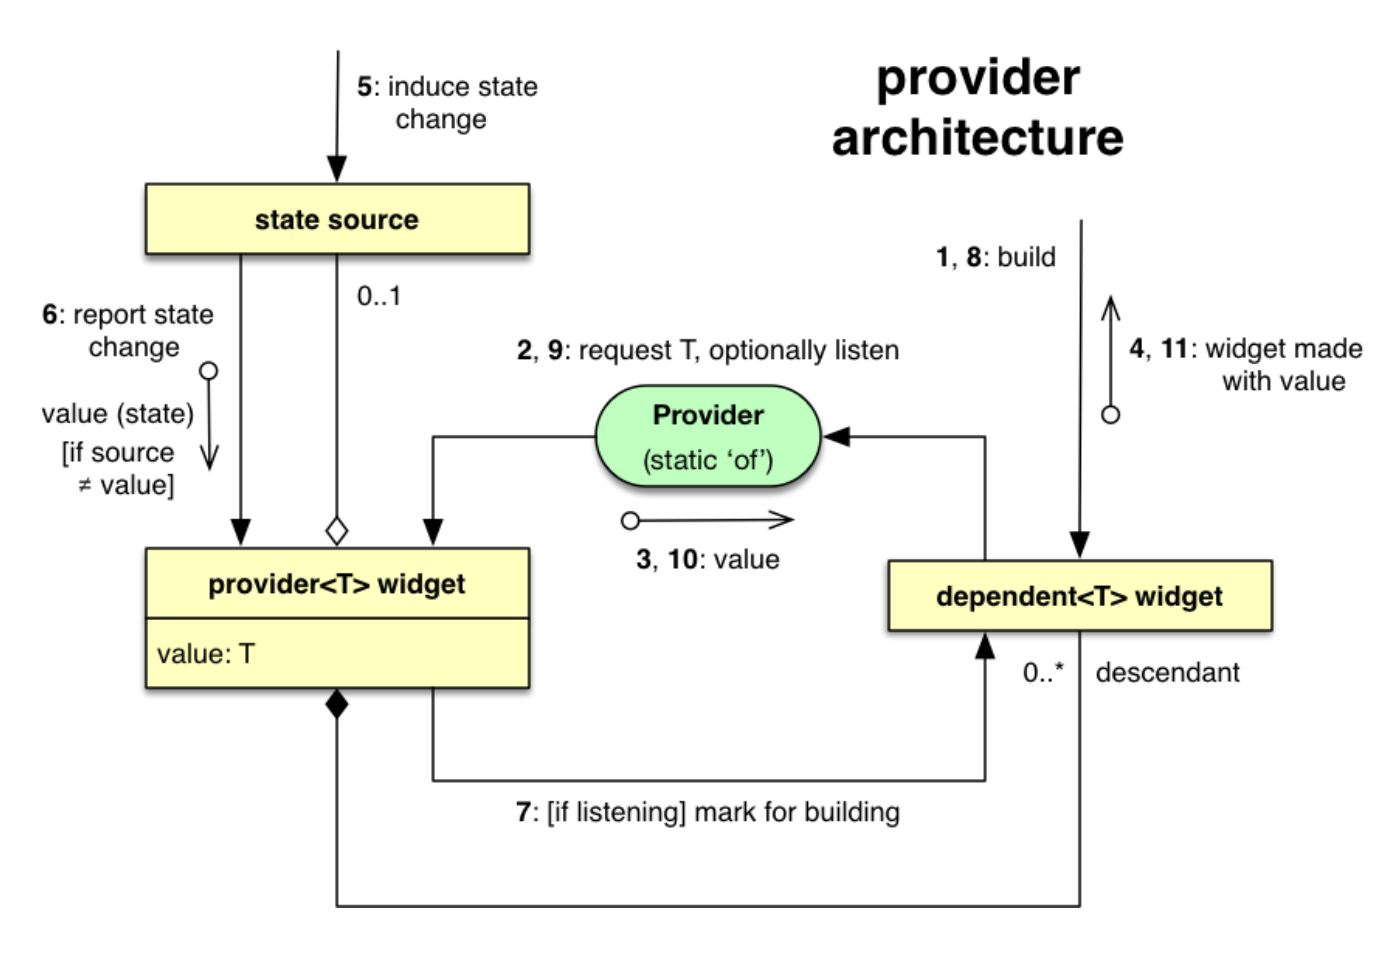
\includegraphics[scale=0.5]{provider}
		\caption[Provider - Architettura complessiva]{Architettura complessiva del pattern Provider\cite{provider_first}.}
		\label{figura:provider}
	\end{center}
\end{figure}

L'oggetto \verb|Consumer<T>| specifica che, al cambiamento di stato, deve essere aggiornato il Widget tree da quel punto in poi, evitando così di ricaricare i alcuni Widget immutabili. Queste tecniche permettono di non aggiornare eventuali Widget che si trovano a dei livelli superiori del Widget tree totale dell'applicazione, infatti, posizionare l'oggetto \verb|Consumer| o chiamare il metodo \verb|Provider.of<T>(context)| vicino alla radice del Widget tree complessivo, potrebbero provocare dei rallentamenti dell'applicazione. La problematica che nessuno di questi due metodi risolve è l'eventuale presenza di uno o più Widget che non devono essere aggiornati, ma che fanno comunque parte del sotto albero di \verb|Consumer| o di \verb|Provider.of<T>(context)|. È possibile ovviare a questo problema, specificando il valore del parametro \verb|listen| nel seguente modo: \verb|Provider.of<T>(context, listen: false)|. Così facendo, il Widget comunica al framework che è soltanto interessato a ricevere i dati dal Provider e che non necessita di essere ricostruito dal motore di rendering.

\subsubsection{Aggiornamento dello stato}
L'aggiornamento dello stato sfrutta i benefici che offre la programmazione reattiva. Possono venire utilizzati gli \verb|Stream|, i \verb|Future|, i \verb|ChangeNotifier| e i \verb|ValueNotifier|. Tutti questi oggetti permettono di comunicare istantaneamente i cambiamenti che rilevano. Così facendo, permettono di avere un flusso di dati che vengono resi disponibili al livello di presentazione dell'applicazione in tempo reale. L'\textit{aggiornamento dello stato} verrà descritto con maggior dettaglio nella spiegazione dedicata al pattern finale dell'applicazione.

\subsection{BLoC}
\subsubsection{Strutturazione del BLoC}
\begin{figure}
	\begin{center}
		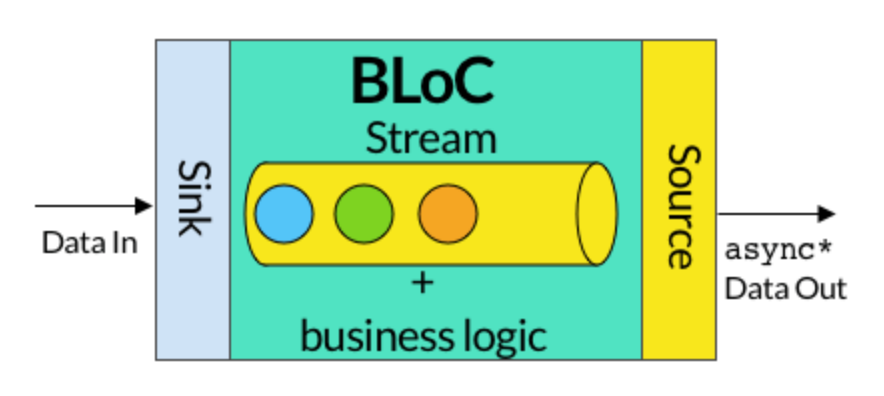
\includegraphics[scale=0.7]{bloc_architecture}
		\caption[BLoC - Architettura complessiva]{Architettura complessiva del pattern BLoC.}
		\label{figura:bloc_architecture}
	\end{center}
\end{figure}

Il \textbf{BLoC} è un sistema di \textit{state management}, consigliato dagli stessi sviluppatori di Google. Aiuta a gestire lo stato e ad accedere ai dati da una posizione centrale nel progetto. Questo pattern è stato presentato per la prima volta alla conferenza \textit{DartConf} del 2018 da parte da Google \cite{presentazione_bloc}. Tuttavia, Google non lo considera un pattern ufficiale per la realizzazione di applicazioni in Flutter, ma vuole semplicemente proporre un modello che può essere integrato con altre architetture o utilizzato singolarmente per lo sviluppo di app.

L'intento principale del pattern è quello di mantenere separata la \textbf{business logic} dall'\textbf{interfaccia grafica}. Non a caso, l'acronimo di BLoC è \textbf{Business Logic Components}. È uno dei pattern che vengono maggiormente utilizzati nella realizzazione di applicazioni in Flutter, in quanto permette di avere una struttura \textbf{scalabile} e \textbf{flessibile}. Anche questo pattern, come i precedenti, sfrutta la programmazione reattiva, sia per rilevare immediatamente un'interazione dell'utente, sia per propagare un nuovo stato ai vari Widget dell'applicazione.

Questo pattern può essere considerato come una \textit{pila}: l'entrata della pila si chiama \textbf{sink} e l’uscita si chiama \textbf{stream}. In entrata vengono accettati gli eventi generati dall’applicazione, come ad esempio un tap dell’utente, e in uscita viene ritornato uno stato che può essere utilizzato per propagare il cambiamento nell'albero dei Widget. Sulla base di questi due termini, si può intuire che l'oggetto principale che permette di rendere disponibile il flusso di dati è lo \verb|Stream|. La Figura 6.5 rappresenta graficamente le direzioni dei vari flussi all'interno del pattern.

I componenti principali di questo pattern sono due:
\begin{enumerate}
	\item UI: l'interfaccia grafica con cui l'utente può interagire;
	\item BLoC: la logica dell'applicazione che va a gestire gli eventi della UI e si collega a dei servizi esterni o a delle risorse interne (ad esempio, una API, cache ed altro ancora).
\end{enumerate}

Al verificarsi di un evento nell'interfaccia grafica, questo viene comunicato al BLoC (\textit{sink}), il quale elaborerà l'evento ed eventualmente apporterà un cambiamento di stato. Il BLoC, oltre a gestire gli eventi delle UI, fornisce i dati prelevati da dei servizi esterni e li invia all'interfaccia grafica. L'uso degli \verb|Stream| permette di sfruttare i vantaggi della programmazione reattiva, avendo così un'applicazione performante e reattiva. 

Lo \verb|Stream| viene istanziato dal BLoC (tramite l'oggetto \verb|StreamController|) e viene poi utilizzato dall'interfaccia grafica grazie al Widget \verb|StreamBuilder|. Nel \verb|child| dello \verb|StreamBuilder| viene associato tutto l'albero dei Widget che verrà aggiornato ogni volta che un nuovo dato sarà disponibile.

\begin{figure}
	\begin{center}
		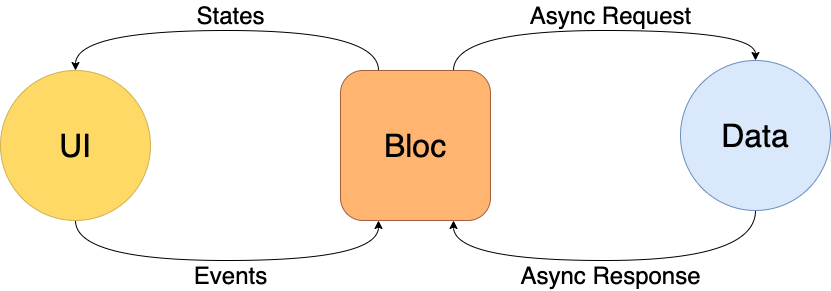
\includegraphics[scale=0.4]{bloc_architecture_2}
		\caption[BLoC - Flusso di dati e di eventi]{Rappresentazione del flusso di dati e di eventi.}
		\label{figura:bloc_architecture_2}
	\end{center}
\end{figure}

\subsubsection{Integrazione del pattern Provider}
Il BLoC è un componente che deve essere inserito nel Widget tree per poter essere usufruito. Pertanto, viene utilizzato il pattern \textit{Provider} a supporto del BLoC, il quale appunto permette di inserirlo all'interno dell'albero dei Widget. In particolare, il BLoC dovrà essere inserito prima dello \verb|StreamBuilder|, in quanto quest'ultimo dipende strettamente dallo \verb|Stream| dichiarato nel BLoC.

L'architettura così descritta definisce una struttura sufficientemente rigida da poter vincolare lo sviluppatore a seguire il flusso \textit{unidirezionale} dei dati. In questo modo, risulta più semplice focalizzarsi sulla realizzazione di un'interfaccia grafica reattiva, senza preoccuparsi della logica che deve essere implementata. Dualmente, nella business logic non è necessario conoscere come verrà realizzata l'interfaccia grafica: ci si concentra invece nel ricevere gli eventi dalla UI e in base ad essi, svolgere le azioni corrispondenti.

Un vincolo che è bene rispettare, è l'implementazione del metodo \verb|dispose()|. Questo metodo viene chiamato quando il BLoC deve essere deallocato e pertanto è necessario chiudere correttamente lo \verb|Stream|, per evitare di causare degli errori nell'applicazione. L'ambiente di sviluppo stesso (che sia Android Studio, IntelliJ, Visual Studio Code o altri) genera un \textit{warning} se nella classe del BLoC non viene mai chiuso lo \verb|Stream|.

Oltre alla rigidità della struttura, è concessa anche una certa flessibilità nella realizzazione dei componenti: un Widget complesso può essere scomposto in Widget più semplici, in modo che siano più facili da gestire e da riusare. Ogni Widget scomposto possiede il proprio BLoC. Quindi è possibile realizzare un componente, con il rispettivo BLoC, ed inserirlo in differenti schermate dell'applicazioni con molta facilità.

Questa architettura impone il rispetto di una regola fondamentale: \textbf{non è possibile condividere} lo stesso BLoC per Widget differenti. Questo dubbio può sorgere allo sviluppatore in situazioni in cui si verifica la necessità di condividere gli stessi dati a due o più Widget differenti contemporaneamente. Risulta naturale, in tale situazione, collegare tutti i Widget sotto un unico BLoC. Tuttavia questa \textit{non è una buona pratica} di programmazione. La condivisone di un BLoC per più schermate può generare diverse problematiche, ad esempio:
\begin{enumerate}
	\item L'aggiornamento di una schermata provoca l'aggiornamento anche delle altre schermate, anche quando non vi è bisogno;
	\item Nel momento in cui viene chiamato il metodo \verb|dispose()|, il BLoC viene deallocato per tutte le schermate con cui è stato condiviso. Quindi navigando tra le schermate, dopo che il BLoC è stato deallocato, si possono verificare degli errori e dei \textit{crash} dell'applicazione.
\end{enumerate}

Un vantaggio dell'integrazione del Provider nel pattern BLoC, è la possibilità di poter istanziare soltanto una volta il BLoC. Una volta istanziato, questo può essere utilizzato in qualsiasi punto dell'applicazione, purché vi sia un \verb|context|. Così facendo, è possibile avere un'ottima flessibilità dell'architettura, evitando di istanziare più volte lo stesso oggetto durante il ciclo di vita dell'applicazione e potendolo utilizzare con una certa facilità, quando lo si necessita.

\subsection{Motivazioni della scelta}
È stato scelto di utilizzare il pattern \textit{BLoC} in quanto l'ho confrontato con le altre architetture disponibili e sono giunto alla conclusione che fosse il pattern ideale per la realizzazione di questa applicazione. Viene sfruttata appieno la programmazione reattiva, caratteristica peculiare del linguaggio, e fornisce una struttura rigida. La rigidità dell'architettura permette di creare delle applicazioni chiare dal punto di vista strutturale. Inoltre permette di avere una certa flessibilità per l'implementazione di funzionalità future.

\section{Architettura proposta}
In questo paragrafo vengono spiegate le problematiche dell'architettura BLoC e le motivazioni che hanno portato a dover attuare delle opportune modifiche per soddisfare i requisiti dell'applicazione.

\subsection{Problematiche del pattern BLoC}
L'applicazione che deve essere realizzata richiede di accedere a dei dati che devono essere forniti da un server, tramite una socket. Questi dati devono essere condivisi tra più schermate: in particolare, si avrà una schermata generale (una \textit{dashboard}), per avere un quadro generale di tutti i dati, e poi vi saranno delle schermate specifiche, che illustreranno soltanto un piccolo set di dati. Tutte queste schermate attingono da un'unica fonte di dati: dalla socket.

Come è stato discusso precedentemente, non è possibile condividere un BLoC per più schermate contemporaneamente. Pertanto, si è dovuti procedere a modificare l'architettura proposta dalla comunità di Flutter, per poterla adattare alle esigenze richieste.

\subsection{Introduzione del Repository pattern}
Per poter risolvere le limitazioni del BLoC, viene integrato il \textbf{Repository} pattern \cite{repository_pattern}. Una spiegazione del Repository è stata data da Martin Fowler nel libro \textit{Patterns of Enterprise Application Architecture}. L'autore spiega che un "\textit{Repository incapsula l'insieme di oggetti persistenti in un archivio dati e le operazioni eseguite su di essi, fornendo una vista più orientata agli oggetti del livello di persistenza.}" Il Repository permette anche di ottenere una netta separazione e una dipendenza unidirezionale tra il dominio e i livelli di mappatura dei dati. Questa concezione è nata in un periodo in cui le applicazioni \textit{enterprise} necessitavano ridurre la duplicazione della logica delle query.

Tuttavia, nel tempo, le esigenze delle applicazioni sono cambiate, in particolare per le applicazioni mobili. In questo contesto, il concetto di Repository viene inteso più come un componente che si interfaccia con un archivio esterno (in generale, qualsiasi altro servizio esterno all'applicazione). In questo caso, il Repository ha il compito di nascondere l'implementazione della logica che permette di interfacciarsi con i servizi esterni. Così facendo, la struttura dell'applicazione risulta essere più flessibile per le modifiche future dei requisiti e il conseguente \textit{refactoring}.

Si possono notare delle differenze sostanziali tra le due definizioni. Per la realizzazione dell'applicazione è stata presa in considerazione l'ultima definizione descritta, le cui motivazioni verranno esposte nella sezione successiva.

\subsection{Architettura modificata}
L'architettura proposta per l'applicazione è costituita dall'integrazione del pattern \textbf{BLoC} con il \textbf{Repository} pattern. Come è stato illustrato precedentemente, nella versione base, il BLoC si occupa di interfacciarsi con la UI da un lato e con i servizi esterni dall'altro. Per sopperire alla problematica della condivisione dei dati ricevuti dalla socket tra le diverse schermate, viene introdotto un Repository tra il BLoC e i servizi esterni. Così facendo si possono ottenere i seguenti vantaggi:
\begin{enumerate}
	\item In questo modo, è possibile utilizzare il Repository come punto di riferimento per la ricezione dei dati per i BLoC. Ovvero, i vari BLoC possono collegarsi ad un Repository comune a tutti e possono ricevere i dati filtrati dal Repository stesso. Infatti, il Repository permette di astrarre dalla sorgente di dati esterna: i BLoC devono soltanto interfacciarsi con il Repository per ottenere i dati, senza preoccuparsi se questi provengano da una socket, da un'API, dalla memoria interna del dispositivo o da qualsiasi altra fonte di dati. Il Repository si preoccupa di interfacciarsi con tali servizi e di confezionare in un certo formato i dati ricevuti, per renderli disponibili e comprensibili ai vari BLoC che vi si collegano;
	\item Grazie a questo nuovo livello di astrazione, tutta la business logic viene alleggerita dal carico di lavoro sostenuto per connettersi ai servizi esterni. Infatti, nel caso in cui in futuro si dovrà cambiare il servizio che permette di ottenere i dati navali, bisognerebbe andare a modificare il codice di ogni singolo BLoC che è stato creato. L'utilizzo invece del Repository, toglie questa responsabilità ai BLoC ed esso diventa l'unico "servizio" a cui i BLoC si devono collegare.
\end{enumerate}

Uno svantaggio dell'integrazione di queste due architetture è appunto l'introduzione di un nuovo livello di astrazione, ovvero, l'introduzione di \textit{overhead}. Per ridurre al minimo questa possibile problematica, viene in aiuto la programmazione reattiva con l'utilizzo degli \textit{flussi} (\verb|Stream| o \verb|ValueNotifier|). Altro fattore che permette di minimizzare questo problema è quello di ridurre al minimo il lavoro che deve svolgere il Repository. I compiti che deve svolgere sono:
\begin{enumerate}
	\item Connettersi con la socket;
	\item Ricevere i dati;
	\item Confezionare i dati ricevuti in un oggetto comprensibile da parte di tutti i BLoC;
	\item Trasmettere i dati in uno \verb|Stream|.
\end{enumerate}

Il lavoro di selezione dei dati viene effettuato dai singoli BLoC, rendendo più veloce il passaggio dei dati dalla sorgente fino ai vari componenti della business logic.

\section{Architettura implementata}
\label{architettura implementata}
Nei paragrafi precedenti, si è andati a descrivere nel particolare le varie architetture, illustrando le motivazioni per cui sono state scelte. Sono state esposte le varie problematiche ed è stata proposta una nuova versione dell'architettura. In questo paragrafo verrà mostrata l'architettura complessiva implementata nell'applicazione.

\subsection{Descrizione}
\begin{figure}
	\begin{center}
		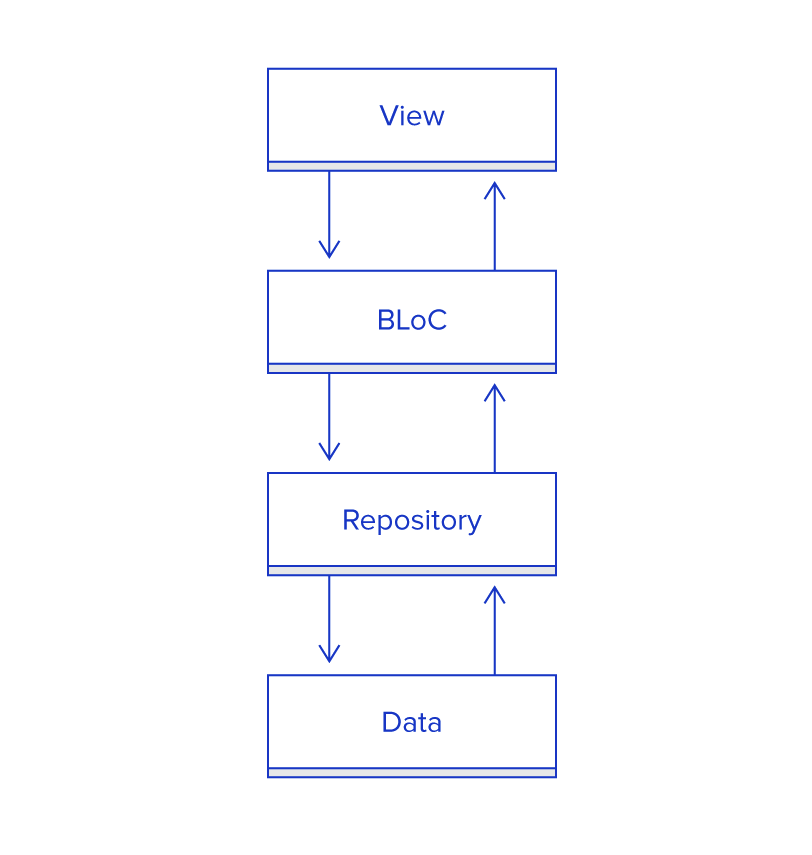
\includegraphics[scale=0.29]{architettura_implementata}
		\caption[Architettura implementata]{Illustrazione degli strati dell'architettura implementata.}
		\label{figura:architettura_implementata}
	\end{center}
\end{figure}

Sulla base di tutte le nozioni che sono state fornite precedentemente, si è giunti ad una struttura finale dell'architettura dell'applicazione. In particolare, gli strati dell'architettura sono (Figura 6.6 \cite{architettura_implementata}):
\begin{enumerate}
	\item \textbf{Interfaccia grafica} (\textbf{View}): tutti quei componenti grafici con cui l'utente può interagire e visualizzare le informazioni richieste;
	\item \textbf{BLoC}: lo strato in cui è contenuta la logica dell'applicazione. Lo logica totale dell'app è data dall'insieme di tutti i BLoC delle singole schermate e dei singoli Widget;
	\item \textbf{Repository}: un livello che si occupa di astrarre il \textit{link} tra i BLoC e i servizi esterni;
	\item \textbf{Servizi esterni}: in questo caso, sono rappresentati dalla socket. In futuro, altri servizi che potrebbero essere inseriti sono, ad esempio, un'API o anche i dati GPS provenienti dal sensore installato sul dispositivo mobile.
\end{enumerate}

\subsection{Integrazione del Repository}
Nell'architettura di base del BLoC, le classi che implementavano la business logic si occupavano di andare a richiedere i dati ai vari servizi esterni. Ora, invece, i vari BLoC si collegano al Repository, che fa da intermediario tra i servizi esterni e i BLoC stessi. L'aggiunta di uno strato ulteriore implica la modifica della modalità di comunicazione tra i BLoC e i servizi. Con il Repository, la comunicazione avviene nel seguente modo;
\begin{enumerate}
	\item Il Repository si collega ai vari servizi esterni, effettua una richiesta sulla base di un particolare evento ricevuto, riceve la risposta e la inoltra in un \verb|ValueNotifier<T>|. Un \verb|ValueNotifier<T>| può essere usato per contenere un singolo valore e avvisare i suoi ascoltatori quando questo cambia;
	\item Al \verb|ValueNotifier<T>| del Repository, si collegano tutti i BLoC di cui necessitano i dati provenienti da questo strato;
	\item Nei BLoC viene inizializzato un \textit{ascoltatore}, che alla ricezione di un nuovo dato nel \verb|ValueNotifier<T>|, chiama una funzione, passandogli come parametro il dato appena ricevuto;
	\item Una volta ricevuto il dato, la funzione del BLoC specifico elimina i dati di cui non necessita (il Repository fornisce tutti i dati provenienti dalla socket) e li propaga nell'interfaccia grafica. La comunicazione tra la UI e i BLoC avviene tramite \verb|Stream|: la comunicazione tra questi due strati non è cambiata dalla versione base del pattern.
\end{enumerate}

L'implementazione dell'architettura così descritta, permette di \textbf{astrarre} dal tipo di servizio che viene utilizzato e permette anche di avere un \textbf{punto di riferimento per la distruzione dei dati} ai vari BLoC. Tutte queste caratteristiche rendono l'architettura adatta per l'applicazione che deve essere implementata.

Per quanto riguarda il passaggio dei dati tra il Repository e i BLoC, si è deciso di non inviare i dati ai BLoC già convertiti e pronti per essere utilizzati. Il motivo è quello di non \textit{sovraccaricare} il Repository, in quanto causerebbe il degrado delle prestazioni. Così facendo, il carico di lavoro viene distribuito tra il Repository e i BLoC.

L'integrazione del Repository pattern nell'architettura avviene grazie all'utilizzo del \textit{Provider}. È possibile fare un discorso analogo a quello che è stato fatto per l'integrazione del Provider nel BLoC. Essendo un componente di \textit{fondamentale} importanza, il Repository viene posto vicino alla radice dell'albero dell'applicazione: venendo utilizzato da diverse schermate durante il ciclo di vita dell'applicazione, nel momento in cui avviene la chiusura dell'app, il Repository sarà uno degli ultimi oggetti che verranno deallocati. In questo modo, le schermate non saranno soggette ad errori, in quanto queste verranno deallocate prima del Repository.

\section{Descrizione dettagliata dell'architettura implementata}
In questa sezione si procede a descrivere dettagliatamente l'architettura implementata, a partire dai componenti più interni, per procedere poi a trattare le parti che gestiscono l'interazione con l'utente.

\subsection{Organizzazione delle classi e dei package}
In questa breve sezione, viene illustrata l'organizzazione dei package e delle varie classi dell'applicazione realizzata.

L'applicazione è stata strutturata seguendo gli strati dell'architettura, ovvero, è stato creato un package per ogni livello dell'architettura.

L'applicazione è stata organizzata nel seguente modo (in ordine alfabetico):
\begin{enumerate}
	\item \textbf{blocs}
		\begin{enumerate}
			\item dashboard
				\begin{enumerate}
					\item \textit{dashboard\_widget\_bloc.dart}
				\end{enumerate}
			\item gps
				\begin{enumerate}
					\item \textit{gps\_bloc.dart}
				\end{enumerate}
			\item location
				\begin{enumerate}
					\item \textit{location\_bloc.dart}
				\end{enumerate}
			\item navigation
				\begin{enumerate}
					\item \textit{navigation\_bloc.dart}
				\end{enumerate}
			\item wind
				\begin{enumerate}
					\item \textit{wind\_bloc.dart}
				\end{enumerate}
			\item \textit{bloc.dart}
		\end{enumerate}
	\item \textbf{models}
		\begin{enumerate}
			\item repository
				\begin{enumerate}
					\item \textit{repository\_data\_model.dart}
					\item \textit{timestamp.dart}
				\end{enumerate}
			\item settings
				\begin{enumerate}
					\item cache
						\begin{enumerate}
							\item \textit{cache.dart}
						\end{enumerate}
					\item server
						\begin{enumerate}
							\item \textit{server\_parameters.dart}
							\item \textit{server\_settings.dart}
							\item \textit{server\_settings\_file.dart}
						\end{enumerate}
				\end{enumerate}
			\item ui
				\begin{enumerate}
					\item \textit{base\_model.dart}
					\item \textit{dashboard.dart}
					\item \textit{gps.dart}
					\item \textit{location.dart}
					\item \textit{navigation.dart}
					\item \textit{wind.dart}
				\end{enumerate}
			\item \textit{acronyms.dart}
		\end{enumerate}
	\item \textbf{repositories}
		\begin{enumerate}
			\item \textit{repository\_socket.dart}
		\end{enumerate}
	\item \textbf{services}
		\begin{enumerate}
			\item \textit{socket\_service.dart}
		\end{enumerate}
	\item \textbf{ui}
		\begin{enumerate}
			\item common\_widgets
				\begin{enumerate}
					\item app\_bar
						\begin{enumerate}
							\item \textit{page\_app\_bar.dart}
							\item \textit{sensor\_data\_app\_bar.dart}
						\end{enumerate}
					\item grid\_box
						\begin{enumerate}
							\item \textit{grid\_box\.widget.dart}
						\end{enumerate}
					\item location
						\begin{enumerate}
							\item \textit{location\_widget.dart}
						\end{enumerate}
				\end{enumerate}
			\item pages
				\begin{enumerate}
					\item dashboard
						\begin{enumerate}
							\item widgets.\textit{dashboard\_widget.dart}
							\item \textit{dashboard\_page.dart}
						\end{enumerate}
					\item gps
						\begin{enumerate}
							\item \textit{gps\_page.dart}
						\end{enumerate}
					\item navigation
						\begin{enumerate}
							\item \textit{navigation\_page.dart}
						\end{enumerate}
					\item settings
						\begin{enumerate}
							\item cache.\textit{cache\_page.dart}
							\item server.\textit{server\_page.dart}
							\item theme.\textit{theme\_page.dart}
							\item \textit{settings\_page.dart}
						\end{enumerate}
					\item wind
						\begin{enumerate}
							\item \textit{wind\_page.dart}
						\end{enumerate}
				\end{enumerate}
		\end{enumerate}
	\item \textbf{utils}
		\begin{enumerate}
			\item ui
				\begin{enumerate}
					\item themes
						\begin{enumerate}
							\item \textit{custom\_theme.dart}
							\item \textit{default\_theme.dart}
							\item \textit{high\_contrast\_theme.dart}
							\item \textit{theme\_handler.dart}
							\item \textit{themes.dart}
						\end{enumerate}
					\item \textit{colors\_palette.dart}
				\end{enumerate}
		\end{enumerate}
	\item \textbf{\textit{main.dart}}
\end{enumerate}

\subsection{Modelli}
In questa sezione vengono descritti tutti i modelli utilizzati dai vari strati dell'applicazione.

\subsubsection{Acronyms}
Questa è una semplice classe contente delle mappe \textit{acronimo - nome del dato} che vengono utilizzate nelle schermate dell'applicazione. I dati forniti dalla socket sono espressi sotto forma di \textit{acronimi}. Tuttavia in alcune sezioni dell'applicazione è preferibile avere il nome completo del dato che si sta osservando.

La mappa che contiene le associazioni tra acronimi e nomi dei dati dei sensori è la seguente:

\lstset{numbers=left, % vogliamo numerare le righr
  numberstyle=\tiny, % i numeri sono piccoli
  basicstyle=\ttfamily, % usiamo il carattere dattilografico
  columns=fullflexible, % niente emulazioni di allineamento
  backgroundcolor=\color{lightgray}, % colore di sfondo
  language=Java, % linguaggio usato
  }
  \begin{lstlisting}
  static final Map<String, String> _acronyms = {
   	"aws":	"Apparent Wind Speed",
	"awa":       "Apparent Wind Angle",
    	"sog":        "Speed Over Ground",
    	"cog":        "Curse Over Ground",
    	"mh":         "Magnetic Heading",
    	"sow":       "Speed Over Water",
    	"tws":        "True Wind Speed",
    	"twa":        "True Wind Angle",
    	"ih":           "imu_heading",
    	"cang":      "calypso_ang",
    	"camp":     "calypso_amp",
    	"nwang":   "nwang",
  };
  \end{lstlisting}

Tramite il seguente metodo, dato un acronimo, è possibile ottenere il nome completo del dato corrispondente:
\begin{lstlisting}
  static String getSentence(String acronym) {
  	return _acronyms[acronym];
  }
  \end{lstlisting}

\subsubsection{RepositoryDataModel}
Questo oggetto viene utilizzato per incapsulare i dati ricevuti dalla socket. Grazie a questo oggetto è possibile poi trasmetterlo al Repository e ai vari BLoC.

Si può notare dal commento, che l'introduzione di un oggetto \verb|Timestamp| sarà necessario per dei sviluppi futuri, ad esempio, la realizzazione di grafici per i vari sensori. Il timestamp è già presente ogni volta che viene fatta una richiesta alla socket e vengono ricevuti dei dati. Inoltre il timestamp è già presente nella \textit{cache}: è sufficiente utilizzarlo in quanto l'implementazione effettiva è già stata predisposta.

L'oggetto \verb|Timestamp| contiene delle informazioni riguardanti l'ora, il minuto e il secondo in cui i dati sono stati ricevuti dalla socket.

  \begin{lstlisting}
  class RepositoryDataModel {
  	final String jsonData;
  	final Timestamp timestamp;
  	// I need this to know what time I requested the data  
  	// from the socket, so in this way I can build a chart

  	RepositoryDataModel({@required this.jsonData, 
  	@required this.timestamp});

  	@override
  	String toString() {
    		return jsonData + "\n" + timestamp.toString();
  	}
  }
  \end{lstlisting}
  
\subsubsection{BaseModel}
Questa \textit{classe astratta} rappresenta un riferimento comune per tutti i modelli delle specifiche schermate. Per ogni schermata viene associato un particolare modello, nei quali vengono salvati soltanto un piccolo set dei dati forniti dal Repository.

L'unico metodo che dovrà essere implementato dai vari modelli che estenderanno questa classe astratta, è il metodo \verb|toMap()|, che permette alla classe di restituire i dati che essa contiene, sotto forma di una mappa.

\begin{lstlisting}
abstract class BaseModel {
  	Map<String, dynamic> toMap();
}
\end{lstlisting}

\subsubsection{Dashboard}
Il modello che verrà illustrato è il modello che contiene il maggior numero di campi, in quanto la schermata \textit{Dashboard} ha il compito di mostrare all'utente un quadro generale della situazione, presentando tutti i dati ricevuti dal Repository.

Il metodo \verb|Dashboard.fromJson(Map<String, dynamic> json)| estrapola tutti i dati di cui necessita, da un particolare oggetto che li contiene. Questo metodo viene chiamato nel momento in cui vengono ricevuti i dati dal Repository, che sono salvati in formato JSON.

I modelli \verb|Navigation|, \verb|GPS| e \verb|Wind| sono molto simili al modello che è stato presentato. Variano soltanto per numero e tipologia di dati memorizzati al loro interno.

Il modello \verb|Location| è molto simile al modello \verb|Dashboard|, con l'unica differenza che non viene implementato il metodo \verb|fromJson|. Il motivo è che i dati vengono già decodificati dal JSON e vengono poi passati direttamente a tale modello.

\begin{lstlisting}
class Dashboard extends BaseModel {
  final String apparentWindSpeed;
  final String apparentWindAngle;
  final String speedOverGround;
  final String curseOverGround;
  final String magneticHeading;
  final String speedOverWater;
  final String trueWindSpeed;
  final String trueWindAngle;
  final String imu_heading;
  final String calypso_ang;
  final String calypso_amp;
  final String nwang;

  // Constructor
  Dashboard({
    this.apparentWindSpeed = "0",
    this.apparentWindAngle = "0",
    this.speedOverGround = "0",
    this.curseOverGround = "0",
    this.magneticHeading = "0",
    this.speedOverWater = "0",
    this.trueWindSpeed = "0",
    this.trueWindAngle = "0",
    this.imu_heading = "0",
    this.calypso_ang = "0",
    this.calypso_amp = "0",
    this.nwang = "0",
  });

  factory Dashboard.fromJson(Map<String, dynamic> json) {
    return Dashboard(
      apparentWindSpeed: json['aws'],
      speedOverGround: json['sog'],
      curseOverGround: json['cog'],
      magneticHeading: json['mh'],
      speedOverWater: json['sow'],
      trueWindSpeed: json['tws'],
      trueWindAngle: json['twa'],
      imu_heading: json['imu_heading'],
      calypso_ang: json['calypso_ang'],
      calypso_amp: json['calypso_amp'],
      nwang: json['nwang'],
    );
  }

  @override
  Map<String, dynamic> toMap() {
  	...
  }
\end{lstlisting}

\subsubsection{Cache}
Questo modello permette di salvare i dati che vengono ricevuti dalla socket. I dati vengono salvati nella \textit{cache} dal Repository. Le varie schermate utilizzano la cache nella loro fase di inizializzazione, ovvero, recuperano l'ultimo dato salvato per poter istanziare correttamente tutti i componenti della schermata.

La \verb|Cache| è una classe parametrica, quindi è possibile utilizzarla in qualsiasi contesto e con qualsiasi tipo si desideri. I vari dati vengono memorizzati in una lista. I metodi che supporta questa classe sono:
\begin{enumerate}
	\item \verb|save(T data)|: questo metodo si interfaccia con la lista interna e permette di salvare un nuovo dato in tale lista;
	\item \verb|void emptyCache()|: questo metodo permette di svuotare la cache;
	\item \verb|bool isCacheEmpty()|: permette di verificare se la lista interna è vuota o meno;
	\item \verb|T _getLastDataCached()|: è un metodo interno alla classe e permette di ottenere l'ultimo dato che è stato salvato nella lista;
	\item \verb|get lastData|: è un metodo pubblico che utilizza \verb|_getLastDataCached()|. Non è stato utilizzato direttamente il metodo privato in quanto si voleva rendere il nome del metodo più intuitivo;
	\item \verb|List<T> _getDataCached ()|: questo metodo privato permette di ottenere tutto il contenuto della cache;
	\item \verb|get dataCached|: è un metodo pubblico che chiama \verb|_getDataCached ()|. Le motivazioni della creazione di questo metodo sono analoghe a quelle del metodo \verb|get lastData|;
	\item \verb|get size|: questo metodo permette di ottenere quanti dati sono stati salvati nella cache, ovvero, nella lista.
\end{enumerate}

\subsubsection{ServerParameters}
Questa classe permette di salvare tutti i dati necessari per effettuare la connessione al server (indirizzo IP e porta) e per implementare il \textit{polling} (un numero intero che rappresenta l'intervallo di tempo, espresso in secondi). La classe in questione, viene utilizzata dalla schermata \textit{Server}, nella quale è possibile aggiornare i parametri di connessione e del polling. Pertanto, vi sono diversi metodi che vanno ad analizzare i diversi input, in formato stringa, per controllare che rispettino i tipi e i formati richiesti.

\subsubsection{ServerSettingsFile}
Questa classe ha un ruolo di interfaccia tra l'applicazione ed un file di configurazione in JSON. In questo file vengono memorizzati tutti i dati relativi alla connessione e al polling. Così facendo, al riavvio dell'applicazione, se sono state effettuate delle modifiche a tali parametri, questi non vengono persi e possono essere ricaricati.
Le operazioni supportate da questa classe sono:
\begin{enumerate}
	\item \verb|static Future<String> readSettings()|: operazione per leggere dal file JSON;
	\item \verb|static Future<File> writeSettings(String serverSettings)|: metodo che permette di scrivere i dati sul file JSON.
\end{enumerate}

Vengono utilizzati degli oggetti \verb|ServerSettings| per incapsulare tutti i dati che devono essere memorizzati nel file.

\subsubsection{ServerSettings}
Questa classe contiene i medesimi parametri della classe \verb|ServerParameters| e viene utilizzata dalla classe \verb|ServerSettingsFile|. L'oggetto ottenuto per istanziazione di questa classe, possiede un metodo per \textit{codificare} i dati in JSON (\verb|Map<String, dynamic> toJson()|) , in modo da poterli memorizzare nel file, e un metodo per \textit{decodificare} i dati dal file JSON \\(\verb|factory ServerSettings.fromJson(Map<String, dynamic> json)|), in modo da renderli disponibili ai livelli superiori dell'applicazione.

\subsection{Socket}
La \textit{socket} che viene fornita dal server \textit{Argos} tramite la porta \textit{4545}, rappresenta il servizio esterno da cui l'applicazione prende i dati necessari. Nel caso in cui in futuro, i medesimi dati vengano resi disponibili tramite un altro software o un'altra metodologia, sarà sufficiente creare una nuova classe o un nuovo modulo che implementi la connessione al servizio e i metodi per ottenere i dati da tale servizio.

\subsubsection{Metodo getData()}
Questo metodo permette di connettersi ad una socket e di ottenere i dati da essa. Secondo il protocollo che è stato realizzato nel server \textit{Argos}, una volta che il client effettua una richiesta al server, il server invia la risposta e chiude immediatamente la socket. Pertanto, una volta ricevuti i dati (da riga 10 a riga 15), la socket deve essere chiusa correttamente anche dal lato del client (riga 17).

Il metodo appena descritto è un metodo \textit{asincrono}, ovvero, l'applicazione non viene bloccata fino a quando non vengono ricevuti i dati, ma è possibile svolgere altre azioni. Nel caso ci fossero delle problematiche con la connessione ad Internet, l'implementazione che è stata attuata permette di non bloccare l'applicazione.

Il tipo di ritorno è un \verb|Future<RepositoryDataModel>|: \verb|Future| perchè è un metodo asincrono, e \verb|RepositoryDataModel| perchè i dati ricevuti dalla socket vengono incapsulati in un oggetto comune che possa essere comprensibile ai vari BLoC che si collegheranno al Repository. Incapsulare i dati già in questo strato dell'applicazione permette di alleggerire il carico di lavoro del Repository.

  \begin{lstlisting}
  Future<RepositoryDataModel> getData() async {
    Completer<RepositoryDataModel> repositoryData =
        Completer<RepositoryDataModel>();

    try {
      Socket socket = await Socket.connect(serverIPAddress, 
      serverPort, timeout: Duration(seconds: 2));
      log("Socket connected", name: "SailingSocket");

      socket.listen((data) async {
        repositoryData.complete(RepositoryDataModel(
          jsonData: String.fromCharCodes(data).trim(),
          timestamp: Timestamp(dateTime: DateTime.now()),
        ));
      });

      socket.close();
      log("Socket closed", name: "SailingSocket");
    } on SocketException catch (e) {
      rethrow;
    } on TimeoutException catch (e) {
      rethrow;
    }
    return repositoryData.future;
  }
  \end{lstlisting}

\subsection{Repository}
Come è già stato descritto precedentemente, il Repository è uno strato che si interpone tra i BLoC e i vari servizi esterni. Il compito del Repository è quello di nascondere come avviene la connessione con i servizi esterni. Questi possono essere dei \textit{Web services}, una socket o qualsiasi altra fonte di dati. In questo modo, gli altri componenti utilizzano un'interfaccia unica per connettersi al Repository, indipendentemente dalla tipologia di servizio che viene usufruito.

La scelta di introdurre un ulteriore strato all'architettura originale è dovuta anche ad una caratteristica intrinseca del progetto. Un requisito dell'applicazione consiste nell'interrogare periodicamente (eseguire un \textit{polling}) la socket, in modo da avere i dati sempre aggiornati. Inoltre, tutte le schermate dell'applicazione attingono i dati dalla medesima fonte. Non potendo condividere i BLoC per più schermate, la soluzione del Repository risulta essere la scelta più ragionevole. Quindi, nel Repository viene svolto il \textit{polling}, ovvero, periodicamente vengono effettuate delle richieste alla socket sulla base di un parametro che indica quanti secondi devono essere attesi tra una richiesta e quella successiva.

Da un punto di vista più approfondito, nel Repository è presente:
\begin{enumerate}
	\item \verb|ValueNotifier<RepositoryDataModel>|: permette di sfruttare la programmazione reattiva, comunicando, a tutti gli oggetti connessi al Repository, i dati trasmessi attraverso questo oggetto;
	\item \verb|start()|: questo metodo viene invocato nella schermata \textit{Dashboard} e permette di inizializzare il \textit{polling} del servizio;
	\item \verb|stop()|: questo metodo permette di fermare il polling. Viene invocato dall'utente grazie all'interazione con la schermata \textit{Dashboard};
	\item \verb|_getDataFromSocket()|: è un metodo privato (in Dart vengono identificati con il carattere di \textit{underscore}, '\_') che va ad effettuare esplicitamente la chiamata al servizio esterno. Una volta ricevuto il dato, questo viene tramesso nel \verb|ValueNotifier<RepositoryDataModel>|;
	\item \verb|dispose()|: è un metodo che viene invocato nel momento in cui viene deallocato il Repository. È buona pratica chiudere correttamente gli \verb|Stream| e i \verb|ValueNotifier<T>| per evitare che il canale di comunicazione rimanga aperto.
\end{enumerate}

\subsubsection{Metodo start()}
Di seguito verrà illustrato il codice del metodo \verb|start()|. Questo metodo permette di inizializzare l'oggetto \verb|Timer|, tramite il quale sarà possibile implementare il \textit{polling}. I parametri di \verb|Timer.periodic()| (riga 16) sono una funzione da eseguire periodicamente ed il numero di secondi che indica ogni quanto effettuare una richiesta. La funzione \verb|_getDataFromSocket()| viene chiamata per poter ottenere i dati dalla socket.

Si può notare che prima di eseguire \verb|Timer.periodic()|, viene effettuata una chiamata alla funzione \verb|_getDataFromSocket()| (riga 11). Questo viene fatto in quanto, quando viene chiamato \verb|Timer.periodic()|, non viene immediatamente fatta una connessione alla socket, ma si attende un tempo pari a \verb|pollingInterval|. Pertanto, l'utente, dopo aver premuto il bottone di avvio, potrebbe pensare che l'applicazione si sia bloccata o abbia subito un rallentamento. Effettuando una chiamata a \verb|_getDataFromSocket()| è possibile ottenere immediatamente i dati, senza dover attendere.

Le variabili booleane private \verb|_internetConnection| e \verb|_timeoutSocket| sono necessarie per la gestione degli errori di connessine con la socket.

Il tipo di ritorno di questo metodo è un \verb|Future<void>|, in quanto il metodo \verb|_getDataFromSocket()| è anch'esso un \verb|Future<void>|. Inoltre, la parola riservata \verb|await| indica che bisogna attendere il termine della funzione prima di poter continuare ad eseguire il codice del metodo chiamante.
  \begin{lstlisting}
  Future<void> start() async {
    if (!_isTimerActive) {
      _isTimerActive = true;
      log("Start", name: "Repository");

      _internetConnection = true;
      _timeoutSocket = true;

      // Get data immediately at startup stage of the app
      // Don't wait 'pollingInterval' seconds to get the data
      await _getDataFromSocket();

      if (_internetConnection && _timeoutSocket) {
        
        // Start the timer
        _timer = Timer.periodic(
          Duration(seconds: pollingInterval),
          (Timer timer) => _getDataFromSocket(),
        );
      }
    }
  }
  \end{lstlisting}

\subsubsection{Metodo \_getDataFromSocket()}
Il metodo che verrà illustrato rappresenta l'effettivo utilizzo del servizio esterno, in questo caso la socket. Il metodo si interfaccia con le funzionalità messe a disposizione dalla classe \verb|SocketService| (riga 6). Una volta ricevuti i dati, li salva nella \textit{cache} (riga 7) e li trasmette ai vari BLoC attravero il \verb|ValueNotifier<RepositoryDataModel>| (riga 8). In questo modo i BLoC possono elaborare i dati ricevuti e presentarli all'utente.

  \begin{lstlisting}
  Future<void> _getDataFromSocket() async {
    RepositoryDataModel repositoryData;

    if (_internetConnection && _timeoutSocket) {
      try {
        repositoryData = await socketService.getData();
        cache.save(repositoryData);
        socketData.value = repositoryData;

        _internetConnection = true;
        _timeoutSocket = true;
      } on SocketException catch (e) {
        _internetConnection = false;
        print("No internet connection");
      } on TimeoutException catch (e) {
        _timeoutSocket = false;
        print("Timeout");
      }
    }
  }
  \end{lstlisting}

\subsubsection{Metodo stop()}
Questo metodo va a fermare il timer su richiesta esplicita dell'utente, tramite la schermata \textit{Dashboard}. Vengono effettuati i dovuti controlli per evitare di generare errori. L'istruzione a riga 7, permette di fermare il timer.

  \begin{lstlisting}
  void stop() {
    if (_isTimerActive) {
      _isTimerActive = false;
      log("Stop", name: "Repository");

      if (_timer != null) {
        _timer.cancel();
      }
    }
  }
  \end{lstlisting}

\subsubsection{Metodo dispose()}
Questo metodo viene utilizzato nel momento in cui deve essere deallocato il Repository. Viene chiamato il metodo \verb|stop()|, in modo da terminare l'esecuzione del \verb|Timer.periodic()|, per non causare eventuali errori nella chiusura dell'applicazione.

\begin{lstlisting}
void dispose() {
  this.stop();
}
\end{lstlisting}

\subsection{BLoC}
In questa sezione viene descritto il funzionamento del BLoC, a livello di codice. Durante lo sviluppo, si è notato che l'implementazione dei differenti BLoC per ogni schermata (o componente), risultava essere un'attività ripetitiva. Infatti, tutti i BLoC sono accumunati tra loro da una struttura molto simile. Pertanto, si è realizzata un'\textit{astrazione di base} per poter implementare più facilmente tutti i BLoC necessari. Così facendo, per i futuri sviluppi, sarà più semplice andare ad aggiungere dei nuovi BLoC o modificare i BLoC esistenti.

\subsubsection{Classe astratta}
La classe \verb|bloc.dart| va a realizzare un'\textit{astrazione di base} per creare i BLoC necessari ai vari componenti. A partire dal costruttore (dalla riga 2 alla riga 4), si può notare il collegamento diretto con il Repository (\verb|this.repository|) e il collegamento diretto con il flusso di dati proveniente dal Repository\\ (\verb|this.socketData|). In questo canale vengono trasmessi dei dati incapsulati in oggetti \verb|RepositoryDataModel|. Nel corpo del costruttore viene inizializzato un \textit{ascoltatore}: nel momento in cui il Repository invia dei dati nel canale di comunicazione (\verb|ValueNotifier<RepositoryDataModel>|), il BLoC rileverà i nuovi dati ed invocherà il metodo \verb|onReceived|.

Il metodo \verb|onReceived| (dalla riga 13 alla riga 15) si occupa di decodificare, dal formato JSON, il contenuto dell'oggetto ricevuto. Una volta decodificato, i dati vengono trasmessi nello \verb|Stream|, tramite l'oggetto \verb|StreamController|, un oggetto che si occupa di gestire gli stream.

Questa classe astratta è una classe \textit{parametrica} \verb|Bloc<T extends BaseModel>|, che accetta come parametro \verb|T|, soltanto quelle classi che estendono la classe \verb|BaseModel|. Il motivo di questa realizzazione è dovuto ad un aspetto implementativo dell'astrazione. Il metodo \verb|getDataFromJSON| accetta come parametro un oggetto \verb|RepositoryDataModel| e restituisce un risultato di tipo \verb|T|. La classe del tipo di ritorno deve poter estendere la classe \verb|BaseModel|, in quanto gli oggetti che le varie schermate gestiscono, estendono tale classe. Tutti questi aspetti hanno contribuito a realizzare una buona astrazione del concetto di BLoC.

Il metodo \verb|dispose()| (dalla riga 17 alla riga 21) si occupa di:
\begin{enumerate}
	\item Rimuove l'ascoltatore;
	\item Chiudere il canale di comunicazione del\\ \verb|ValueNotifier<RepositoryDataModel>|;
	\item Chiudere lo \verb|StreamController|, ovvero, chiudere il flusso di dati con l'interfaccia grafica.
\end{enumerate}

Di seguito, il codice che implementa le funzionalità basilari del BLoC.
\begin{lstlisting}
abstract class Bloc<T extends BaseModel> {
  Bloc({@required this.repository, @required this.socketData}) {
    socketData.addListener(onReceived);
  }

  final RepositorySocket repository;
  final ValueNotifier<RepositoryDataModel> socketData;
  final StreamController _streamController = 
  StreamController<T>();

  Stream<T> get stream => _streamController.stream;

  void onReceived() {
    _streamController.add(getDataFromJSON(socketData.value));
  }

  void dispose() {
    socketData.removeListener(onReceived);
    socketData.dispose();
    _streamController.close();
  }

  T getDataFromJSON(RepositoryDataModel repositoryData);
}
\end{lstlisting}

\subsubsection{NavigationBloc}
Questo BLoC si interpone tra la schermata \verb|NavigationPage| ed il Repository. La struttura di questo BLoC ha un'impostazione standard che è presente anche nei BLoC \textit{GPS} e \textit{Wind}. L'unico metodo che implementa la classe è il metodo \verb|getDataFromJSON|, necessario per trasformare i dati dal formato JSON all'oggetto \verb|Navigation| (in questo caso).

\begin{lstlisting}
class NavigationBloc extends Bloc<Navigation> {
  NavigationBloc({@required this.repository, 
  @required socketData})
      : super(repository: repository, socketData: socketData);
  final RepositorySocket repository;

  @override
  Navigation getDataFromJSON(
  RepositoryDataModel repositoryModel) {
    Map<String, dynamic> map = jsonDecode(
    repositoryModel.jsonData);
    return Navigation.fromJson(map);
  }
}
\end{lstlisting}

\subsubsection{DashboardWidgetBloc}
Questa classe è molto simile al BLoC \verb|NavigationBloc|. Le uniche differenze sono l'implementazione dei due metodi \verb|start()| (dalla riga 15 alla riga 17) e \verb|stop()| (dalla riga 19 alla riga 21). Questi metodi sono necessari in quanto tramite la schermata \textit{Dashboard}, l'utente può \textit{avviare} o \textit{fermare} le richieste periodiche alla socket (\textit{polling}). I metodi descritti interagiscono direttamente con il Repository.

\begin{lstlisting}
class DashboardWidgetBloc extends Bloc<Dashboard> {
  DashboardWidgetBloc({@required this.repository, 
  @required socketData})
      : super(repository: repository, socketData: socketData);
  final RepositorySocket repository;

  @override
  Dashboard getDataFromJSON(
  RepositoryDataModel repositoryModel) {
    Map<String, dynamic> map = jsonDecode(
    repositoryModel.jsonData);
    return Dashboard.fromJson(map);
  }

  void start() {
    repository.start();
  }

  void stop() {
    repository.stop();
  }
}
\end{lstlisting}

\subsection{View}
In questa sezione vengono presentate tutte le implementazioni delle varie schermate dell'applicazione, illustrando anche le motivazioni delle scelte grafiche attuate.

\subsubsection{Navigation}
In questa schermata vengono visualizzati i dati relativi alla \textit{navigazione}, in particolare è possibile monitorare i seguenti dati:
\begin{enumerate}
	\item \textbf{Apparent Wind Speed}
	\item \textbf{Apparent Wind Angle}
	\item \textbf{Magnetic Heading}
	\item \textbf{Speed Over Water}
\end{enumerate}

La struttura della classe che implementa questa schermata (\verb|NavigationPage|) risulta essere molto compatta e semplice, grazie all'astrazione che è stata fatta sui BLoC e all'astrazione di alcuni componenti grafici comuni. Di seguito viene illustrato il codice della schermata in questione.

\newpage

\begin{lstlisting}
class NavigationPage extends StatefulWidget {
  NavigationPage(
      {Key key, @required this.navigationBloc, 
      @required this.themeHandler})
      : super(key: key);
  final NavigationBloc navigationBloc;
  final ThemeHandler themeHandler;

  static Widget create(BuildContext context) {
    final RepositorySocket repository =
        Provider.of<RepositorySocket>(context, listen: false);

    final ThemeHandler themeHandler =
        Provider.of<ThemeHandler>(context, listen: false);

    return Provider<NavigationBloc>(
      create: (_) => NavigationBloc(
          repository: repository, 
          socketData: repository.socketData),
      dispose: (context, bloc) => bloc.dispose(),
      child: Consumer<NavigationBloc>(
          builder: (context, bloc, _) =>
              NavigationPage(navigationBloc: bloc, 
              themeHandler: themeHandler)),
    );
  }

  @override
  State<StatefulWidget> createState() => _NavigationPageState();
}

class _NavigationPageState extends State<NavigationPage>
    with AutomaticKeepAliveClientMixin<NavigationPage> {
  @override
  bool get wantKeepAlive => true;

  @override
  Widget build(BuildContext context) {
    super.build(context);
    return GridBox(
      bloc: widget.navigationBloc,
      themeHandler: widget.themeHandler,
      initialData: Navigation(),
    );
  }
}
\end{lstlisting}

\verb|NavigationPage| è una classe che estende \verb|StatefulWidget|, in quanto dovrà gestire eventuali cambiamenti di stato dell'applicazione. Il metodo \\ \verb|static Widget create(BuildContext context)| (dalla riga 9 alla riga 26) viene chiamato dal \verb|main.dart| e permette di inizializzare correttamente sia la schermata di navigazione che il rispettivo BLoC. In particolare, è possibile notare che viene utilizzato il \verb|Repository| grazie al \verb|Provider|, specificando il parametro \verb|listen:false|. In questo modo si specifica al Provider che all'arrivo di un nuovo dato, la grafica non deve essere aggiornata. Allo stesso modo viene utilizzato il \verb|ThemeHandler|.

\begin{figure}
	\begin{center}
		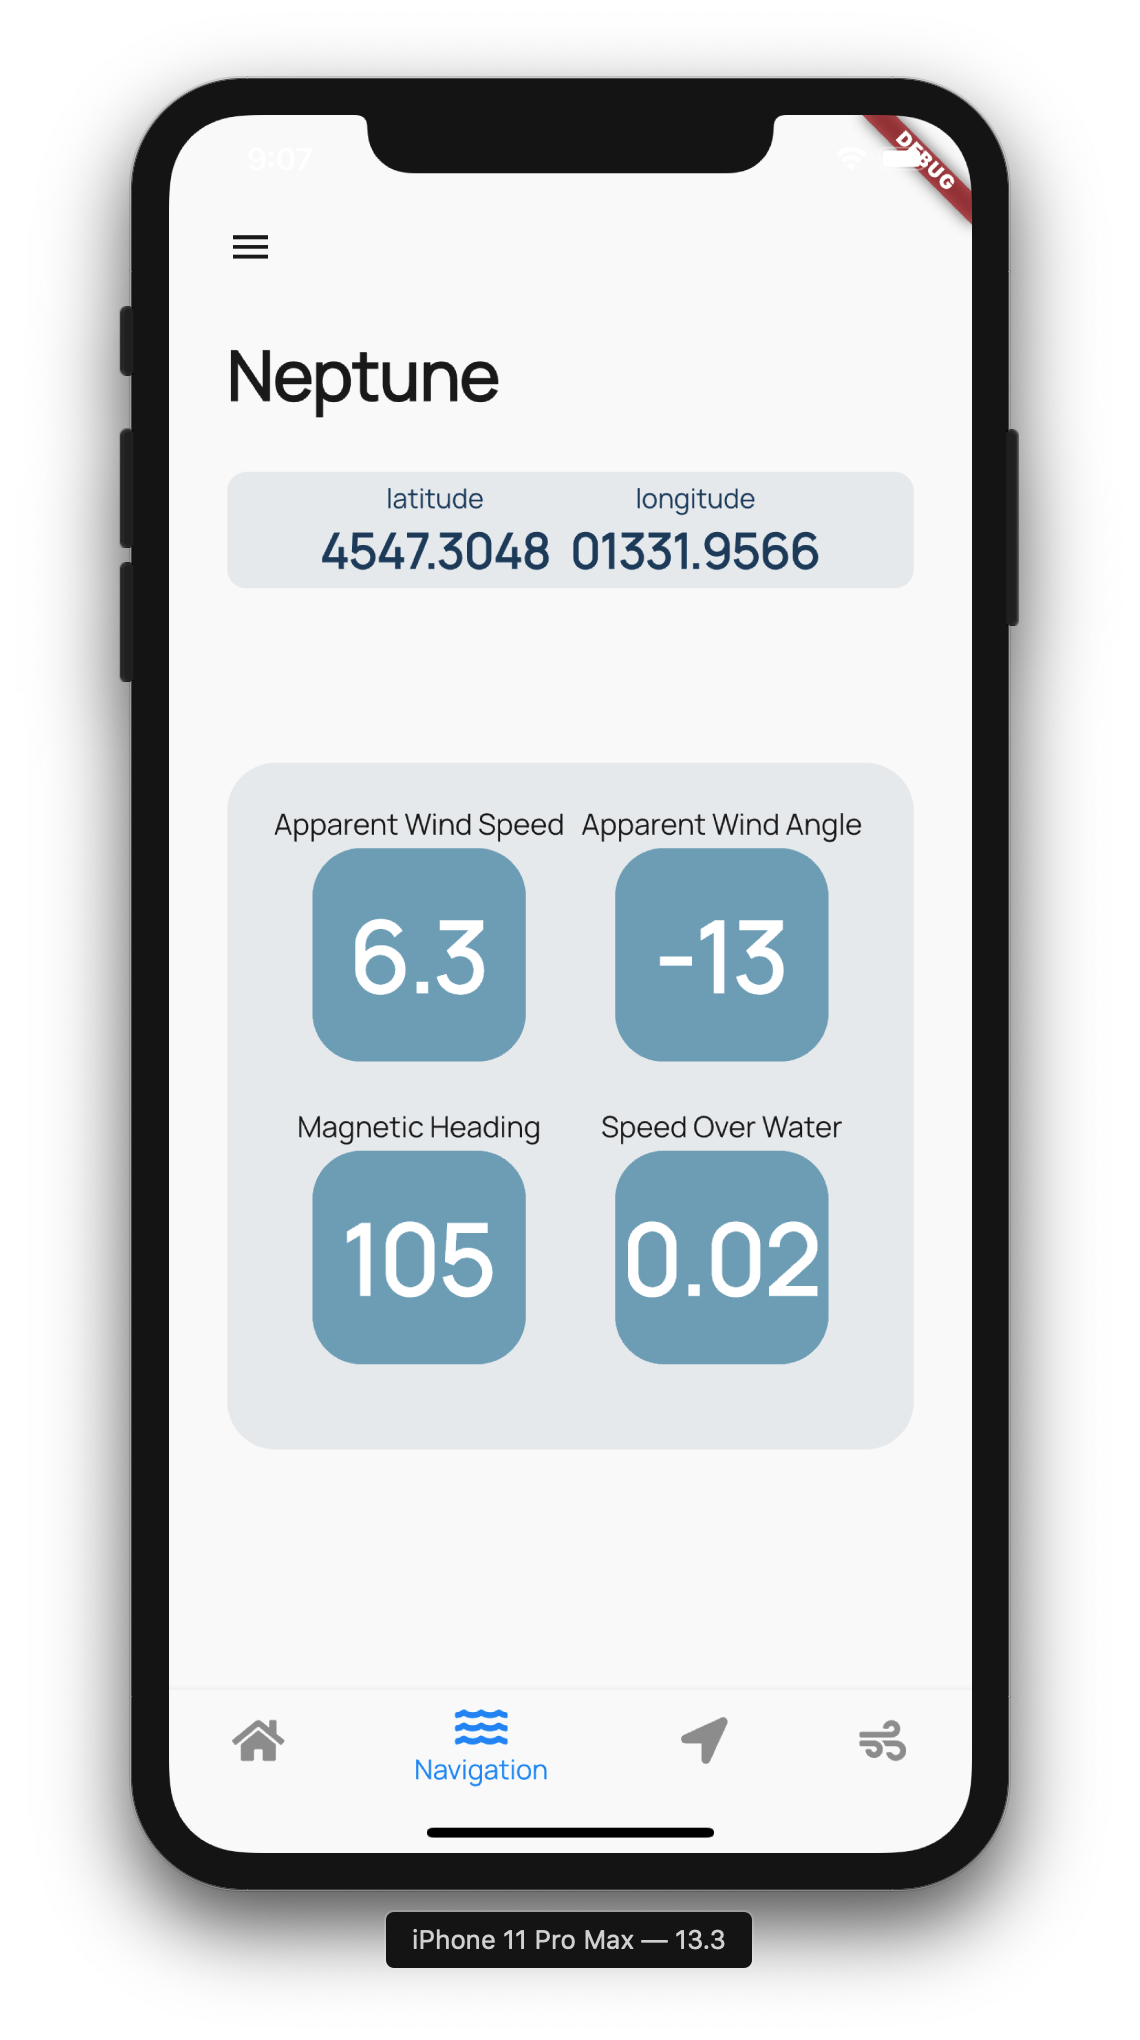
\includegraphics[scale=0.34]{navigation}
		\caption[Screenshot - Navigation]{Screenshot della schermata \textit{Navigation}.}
		\label{figura:navigation}
	\end{center}
\end{figure}

Sulla base dell'architettura proposta (sezione \textit{\nameref{architettura implementata}}), il BLoC relativo alla schermata deve essere posizionato prima dell'oggetto \verb|NavigationPage|. Infatti, nel metodo \verb|create| viene ritornato prima il\\ \verb|Provider<NavigationPage>| e poi, come figlio di quest'ultimo, \verb|NavigationPage|. La schermata viene incapsulata nel \verb|Consumer|: una spiegazione approfondita è stata redatta nella sezione \textit{\nameref{consumer}}.

Nella classe privata \verb|_NavigationPageState| viene utilizzata la \textit{mixin}\\ \verb|AutomaticKeepAliveClientMixin<T>| (un approfondimento è presente nell'appendice \ref{cap:B}), necessario per evitare di ricaricare i dati anche quando si cambia schermata. Il metodo \verb|build()| (dalla riga 37 alla riga 45) ritorna un Widget comune: il \verb|GridBox|. A questo Widget viene passato il corrispondente BLoC, la classe che gestisce i temi e i dati che devono essere visualizzati appena istanziato il Widget. In particolare, \verb|initialData| è necessario nel momento in cui viene avviata l'applicazione e non è stata ancora effettuata alcuna richiesta alla socket. Quindi, non avendo a disposizione dei dati provenienti dal server, il Widget deve comunque illustrare dei dati iniziali. Questi dati iniziali vengono forniti appunto tramite il parametro \verb|initialData|.

\newpage

\subsubsection{GPS e Wind}
\begin{figure}[htp]
	\centering
	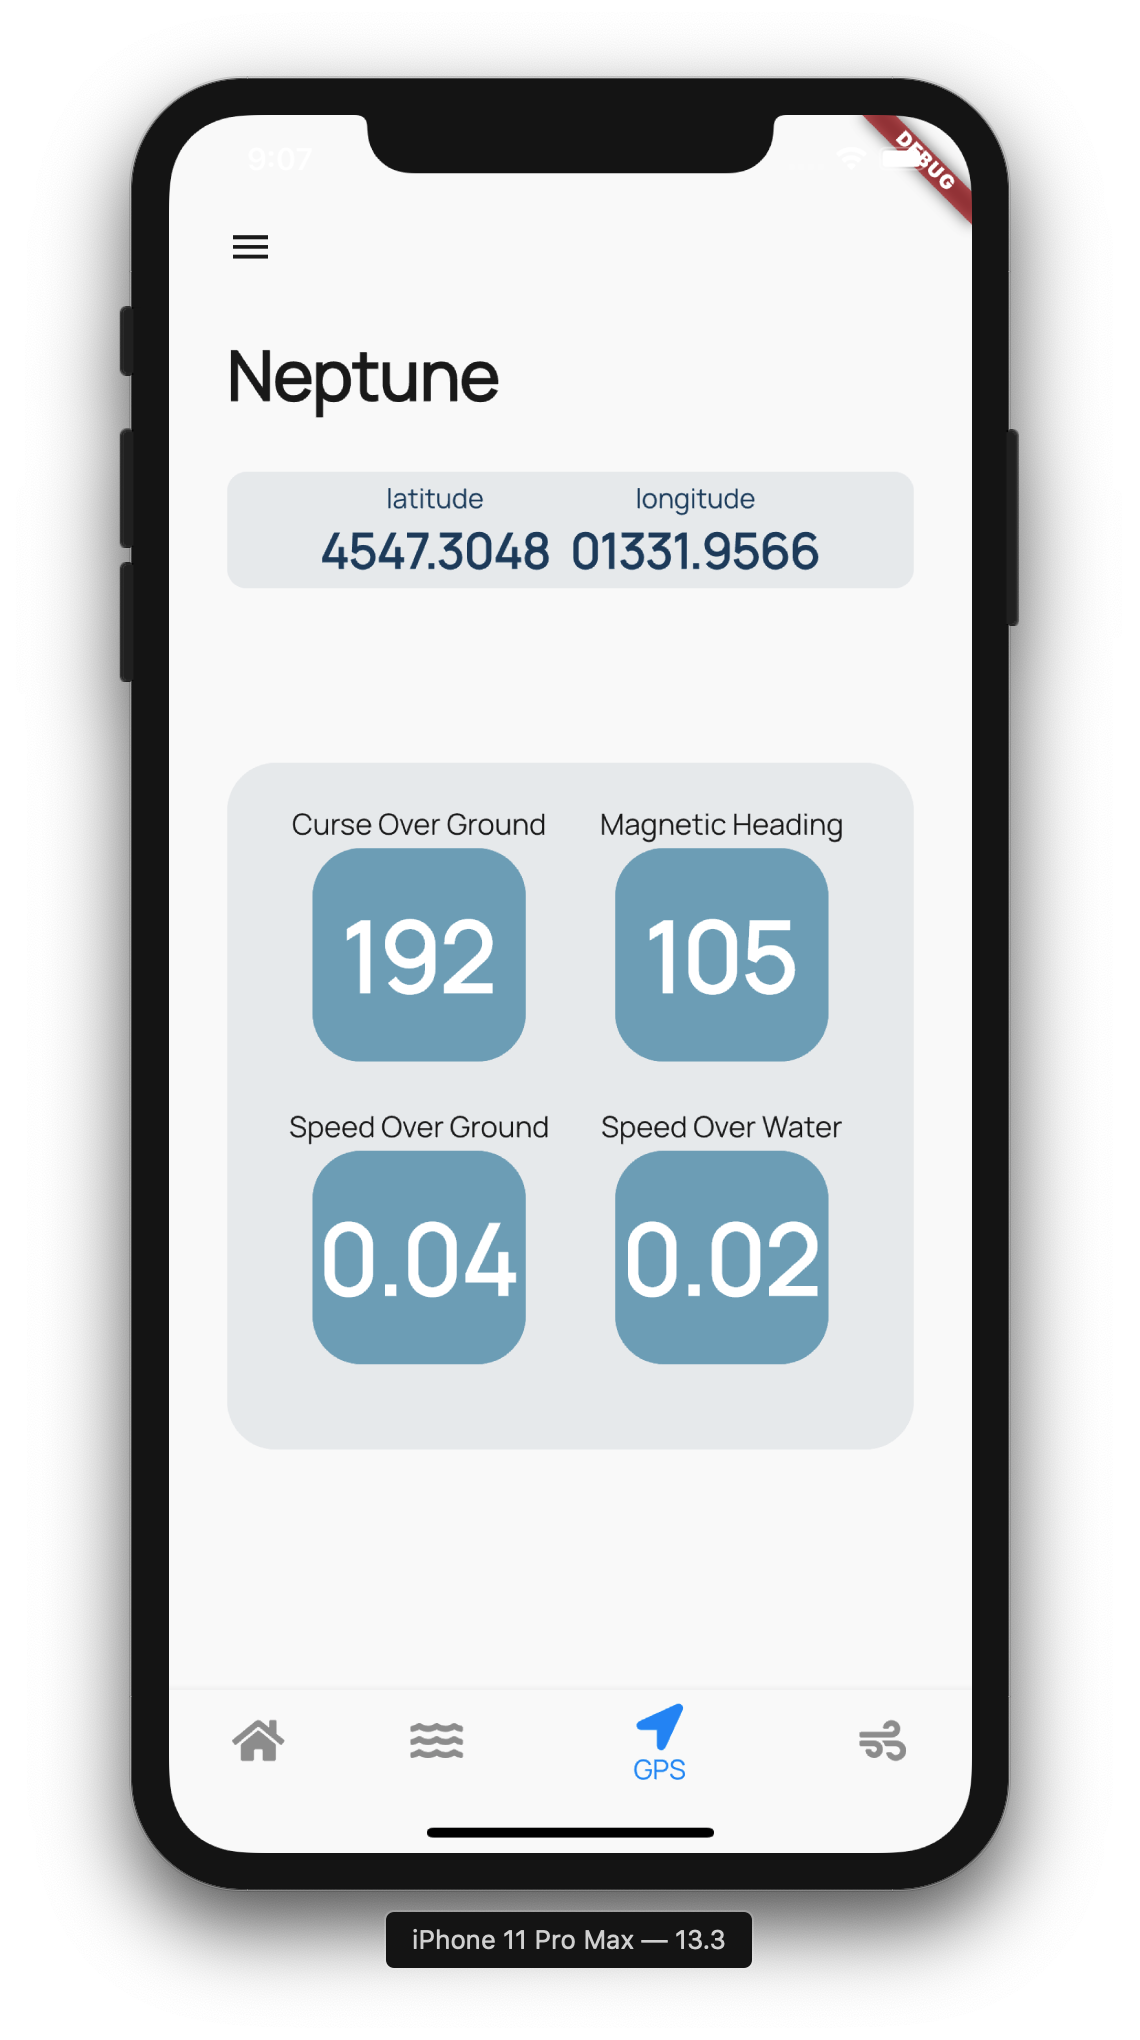
\includegraphics[scale=0.34]{gps}
	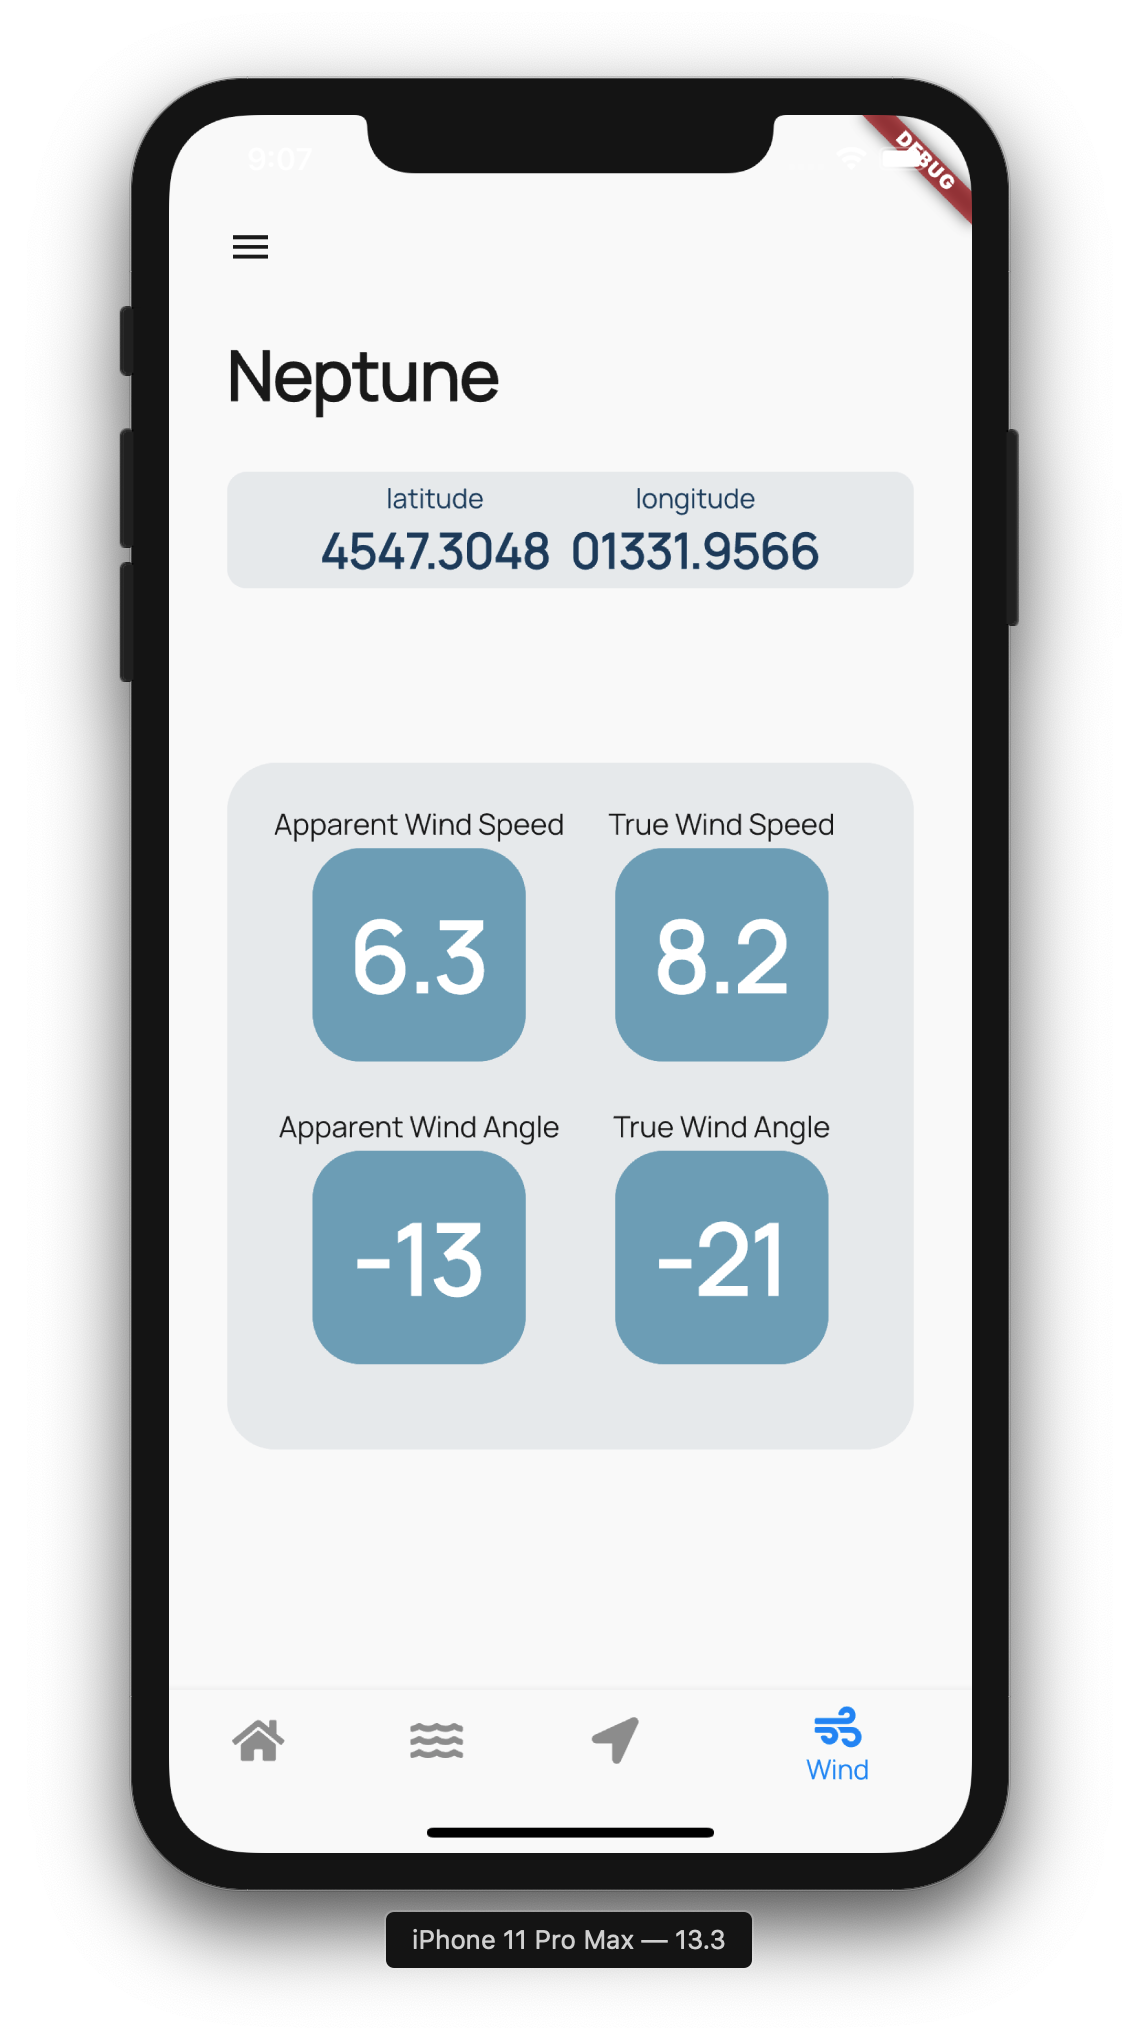
\includegraphics[scale=0.34]{wind}
	\caption[Screenshot - Drawer e della schermata Settings]{Screenshot della schermata \textit{GPS} (a sinistra) e della schermata di \textit{Wind} (a destra).}\label{xyz}
\end{figure}

Nella schermata \textbf{GPS} è possibile monitorare i dati relativi alla geolocalizzazione (le coordinate vengono prese dal sensore GPS installato sul Raspberry e non dal dispositivo in cui viene utilizzata l'applicazione). Mentre, nella schermata \textbf{Wind} è possibile visualizzare i dati relativi al vento, come ad esempio la reale velocità del vento.

In particolare, nella schermata \textit{GPS} è possibile monitorare i seguenti dati:
\begin{enumerate}
	\item \textbf{Curse Over Ground}
	\item \textbf{Magnetic Heading}
	\item \textbf{Speed Over Ground}
	\item \textbf{Speed Over Water}
\end{enumerate}

Nella schermata \textit{Wind} l'utente può controllare i seguenti dati:
\begin{enumerate}
	\item \textbf{Apparent Wind Speed}
	\item \textbf{True Wind Angle}
	\item \textbf{Apparent Wind Angle}
	\item \textbf{True Wind Angle}
\end{enumerate}

La struttura di queste schermate segue il modello semplice e compatto della schermata \textit{Navigation}.

\subsubsection{Dashboard}
Questa è la schermata che l'utente vede all'apertura dell'applicazione. Il principale obiettivo di questa schermata è quello di fornire all'utente un quadro generale della situazione. In questo modo può monitorare tutti i dati riguardanti la navigazione. Inoltre da questa schermata, l'utente può avviare o fermare il \textit{polling} dei dati, ovvero, può avviare o fermare le richieste verso la socket quando lo ritiene opportuno.

Nonostante questa sia la schermata principale dell'applicazione, la spiegazione di essa viene effettuata soltanto ora in quanto possiede una struttura differente rispetto allo schema \textit{standard} delle schermate \textit{Navigation}, \textit{GPS} e \textit{Wind}. Le altre schermate seguono un approccio più semplice: ad ogni pagina è associato un BLoC. Come è possibile notare dal codice della classe \verb|DashboardPage|, non è presente alcun riferimento ad un qualche BLoC. Questa schermata è stata strutturata in modo che la \verb|DashboardPage| possa integrare diversi Widget per comporre una grafica complessiva. Ogni componente grafico al suo interno possiede il proprio BLoC (sia \verb|LocationWidget| che \verb|DashboardWidget|, riga 23 e 24).
\begin{lstlisting}
class DashboardPage extends StatefulWidget {
  DashboardPage({Key key}) : super(key: key);

  @override
  State<StatefulWidget> createState() => _DashboardPageState();
}

class _DashboardPageState extends State<DashboardPage>
    with AutomaticKeepAliveClientMixin<DashboardPage> {
  @override
  bool get wantKeepAlive => true;

  @override
  Widget build(BuildContext context) {
    super.build(context);
    return _buildUI();
  }

  Widget _buildUI() {
    return ListView(
      shrinkWrap: true,
      children: <Widget>[
        LocationWidget.create(context),
        DashboardWidget.create(context),
      ],
    );
  }
}
\end{lstlisting}

Osservando il codice relativo alla classe \verb|DashboardWidget|, è possibile notare che la struttura di  questo componente è sostanzialmente uguale a quella della schermata \textit{Navigation}. Grazie alla pagina \textit{Dashboard}, si possono vedere i benefici e i vantaggi dell'utilizzo di un'architettura BLoC: non è necessario che ogni singola schermata possieda il proprio BLoC, ma possono essere creati dei BLoC per componenti di dimensioni più piccole. Successivamente, questi componenti possono essere assemblati in un unico Widget, come nel caso della \textit{Dashboard} con i Widget \textit{Location} e \textit{DashboardWidget}.

\begin{lstlisting}
class DashboardWidget extends StatefulWidget {
  DashboardWidget(
      {Key key, @required this.dashboardBloc, 
      @required this.themeHandler})
      : super(key: key);
  final DashboardWidgetBloc dashboardBloc;
  final ThemeHandler themeHandler;

  static Widget create(BuildContext context) {
    final RepositorySocket repository =
        Provider.of<RepositorySocket>(context, listen: false);

    final ThemeHandler themeHandler =
        Provider.of<ThemeHandler>(context, listen: false);

    return Provider<DashboardWidgetBloc>(
      create: (_) => DashboardWidgetBloc(
          repository: repository, 
          socketData: repository.socketData),
      dispose: (context, bloc) => bloc.dispose(),
      child: Consumer<DashboardWidgetBloc>(
          builder: (context, bloc, _) =>
              DashboardWidget(dashboardBloc: bloc, 
              themeHandler: themeHandler)),);
  }

  @override
  State<StatefulWidget> createState() => _DashboardWidgetState();
}

class _DashboardWidgetState extends State<DashboardWidget>
    with AutomaticKeepAliveClientMixin<DashboardWidget> {
  @override
  bool get wantKeepAlive => true;

  @override
  Widget build(BuildContext context) {
    super.build(context);
    return StreamBuilder<Dashboard>(
      stream: widget.dashboardBloc.stream,
      initialData: Dashboard(),
      builder: (context, snapshot) {
        return _buildGrid(snapshot.data.toMap());
      },
    );
  }

  Widget _buildGrid(Map<String, dynamic> dashboardData) { ... }

  Widget _buildButtons() { ... }

  Widget _buildSingleBox(Map<String, dynamic> dashboardData, 
  String key) { ... }
}
\end{lstlisting}

\begin{figure}[htp]
	\centering
	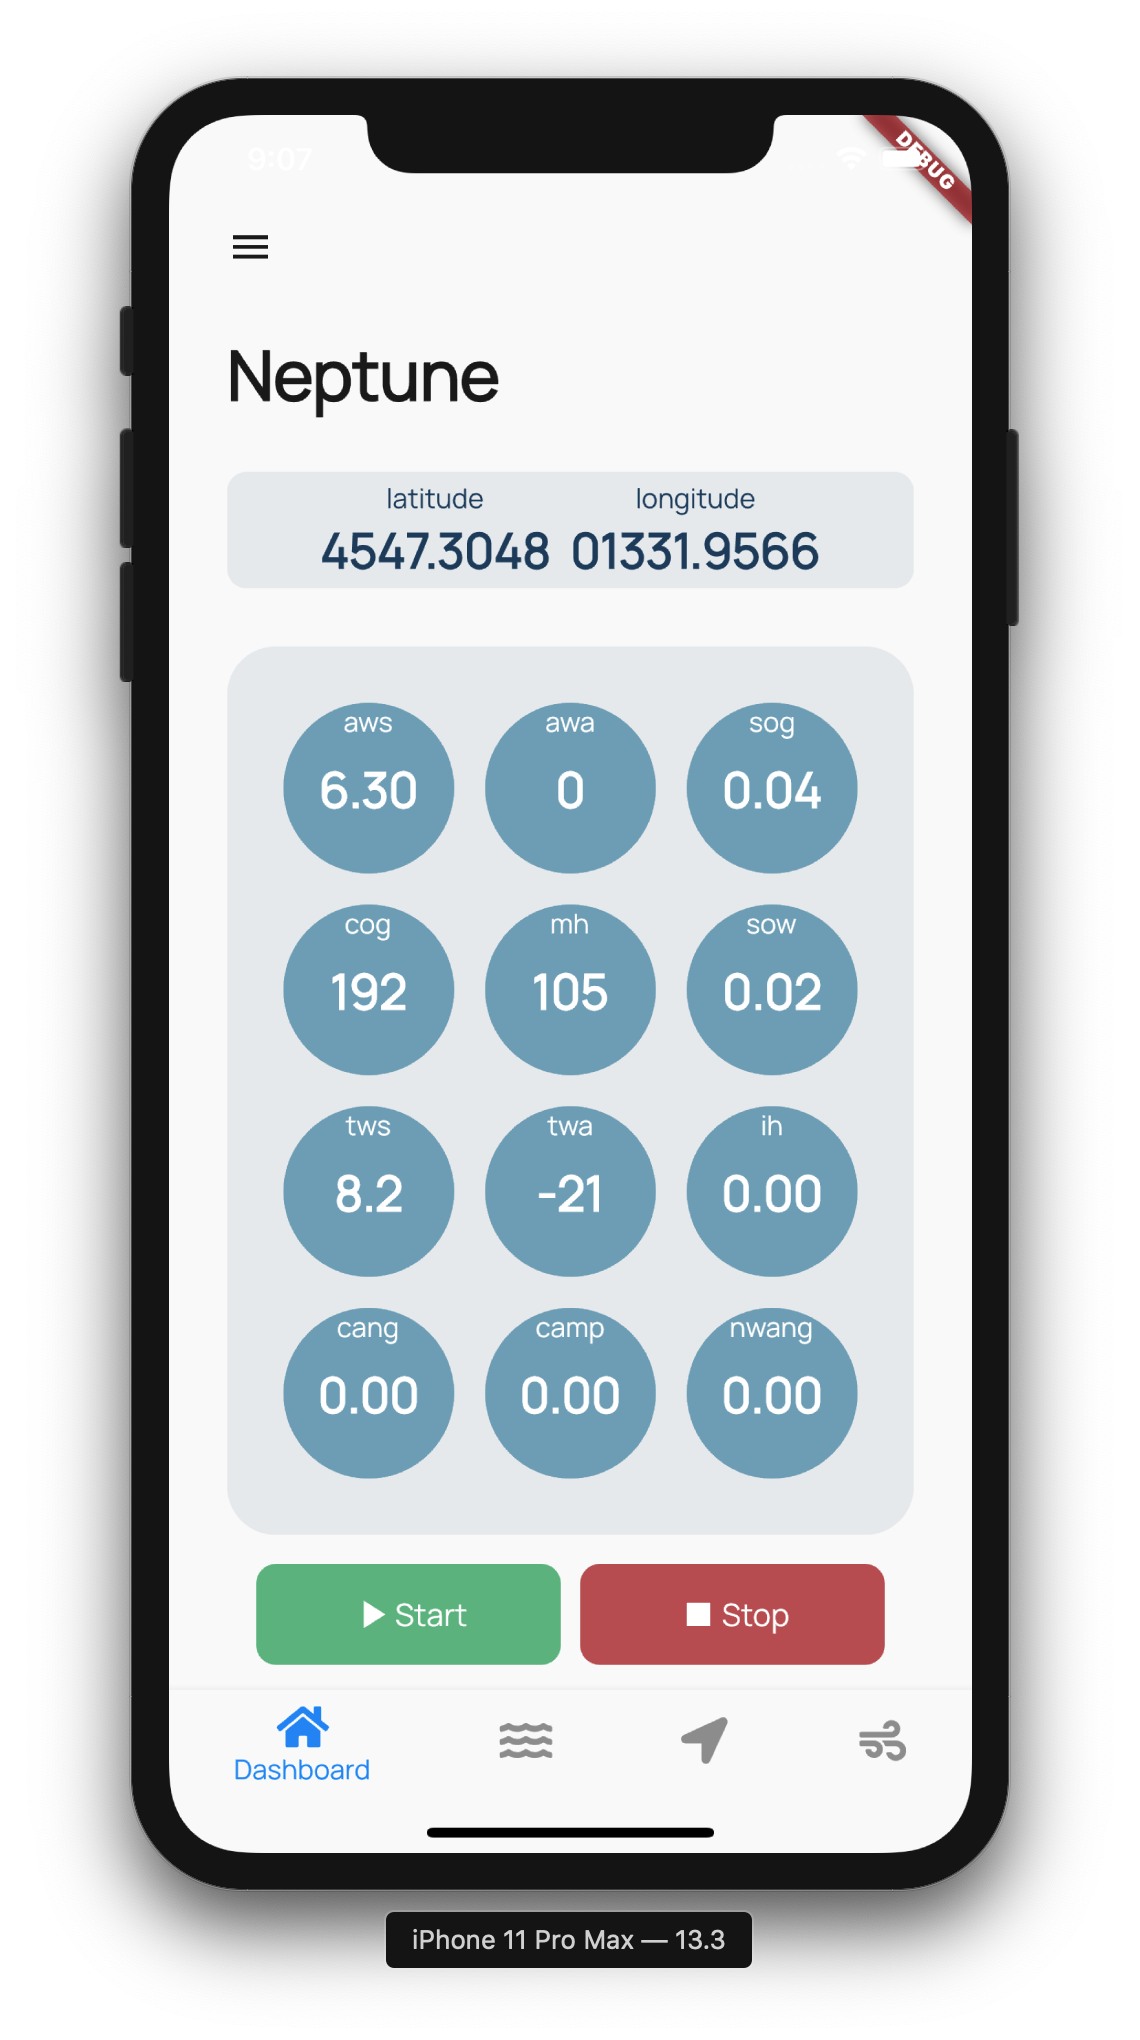
\includegraphics[scale=0.35]{dashboard}
	\caption[Screenshot - Dashboard]{Screenshot della schermata \textit{Dashboard}.}\label{xyz}
\end{figure}

\newpage

\subsubsection{Settings}
Questa schermata presenta una lista delle varie impostazioni che possono essere modificate dall'utente. In questa versione dell'applicazione, possiamo notare tre opzioni:
\begin{enumerate}
	\item \textbf{Cache}
	\item \textbf{Server}
	\item \textbf{Theme}
\end{enumerate}

Facendo \textit{tap} su una di queste opzioni, l'utente verrà portato sulla schermata corrispondente. Per accedere alla schermata delle impostazioni, si deve accedere al \textit{drawer}, posto in alto a sinistra dell'applicazione.

Di seguito viene presentato il codice di questa schermata. È possibile notare la mappa \verb|options| (dalla riga 10 alla riga 29) che va a creare delle associazioni tra il nome della schermata, in formato stringa, e l'oggetto che deve essere istanziato nel caso in cui l'utente faccia tap su una di queste opzioni.

Dal codice è possibile notare inoltre la facilità dell'utilizzo dei Widget: nel metodo \verb|build| è presente il Widget \verb|ListView.builder|, il quale permette di iterare su un oggetto \textit{enumerabile}, come ad esempio delle liste. All'interno di tale Widget, viene utilizzato \verb|ListTile|, un componente grafico che permette di realizzare le voci presenti nella schermata \textit{Settings} (Figura 6.10, screenshot a destra). Tutto questo è possibile realizzarlo con poche righe di codice, sfruttando pochi Widget.

\begin{lstlisting}
class SettingsPage extends StatefulWidget {
  final String title = "Settings";

  @override
  State<StatefulWidget> createState() => _SettingsPageState();
}

class _SettingsPageState extends State<SettingsPage>
    with AutomaticKeepAliveClientMixin<SettingsPage> {
  final Map<String, dynamic> options = {
    "cache": {
      "title": Text("Cache"),
      "leading": Icon(Icons.cached),
      "subtitle": Text("Delete the data saved from the app"),
      "page": CachePage(),
    },
    "server": {
      "title": Text("Server"),
      "leading": Icon(Icons.perm_data_setting),
      "subtitle": Text("Choose the server to connect to"),
      "page": ServerPage(),
    },
    "theme": {
      "title": Text("Theme"),
      "leading": Icon(Icons.color_lens),
      "subtitle": Text("Choose the theme of the app"),
      "page": ThemePage(),
    },
  };

  StatefulWidget _getSettingPage(String option) {
    return options[option]["page"];
  }

  @override
  Widget build(BuildContext context) {
    super.build(context);
    return Scaffold(
      appBar: PageAppBar(context: context, title: widget.title),
      body: ListView.builder(
        itemCount: options.length,
        itemBuilder: (ctx, i) {
          return Padding(
            padding: const EdgeInsets.only(
              left: 20.0,
              right: 20.0,
              bottom: 25.0,
            ),
            child: Container(
              decoration: BoxDecoration(
                color: ColorsPalette.softGrey,
                borderRadius: BorderRadius.circular(10.0),
              ),
              child: ListTile(
                leading: options[
                options.keys.toList()[i]]["leading"],
                title: options[
                options.keys.toList()[i]]["title"],
                subtitle: options[
                options.keys.toList()[i]]["subtitle"],
                trailing: Icon(CupertinoIcons.forward),
                onTap: () async {
                  Future<Widget> buildPageAsync() async {
                    return Future.microtask(() {
                      return _getSettingPage(
                      options.keys.toList()[i]);
                    });
                  }

                  Widget page = await buildPageAsync();
                  MaterialPageRoute route =
                      MaterialPageRoute(builder: (_) => page);
                  Navigator.push(context, route);
                },
              ),
            ),
          );
        },
      ),
    );
  }

  @override
  bool get wantKeepAlive => true;
}
\end{lstlisting}

\begin{figure}[htp]
	\centering
	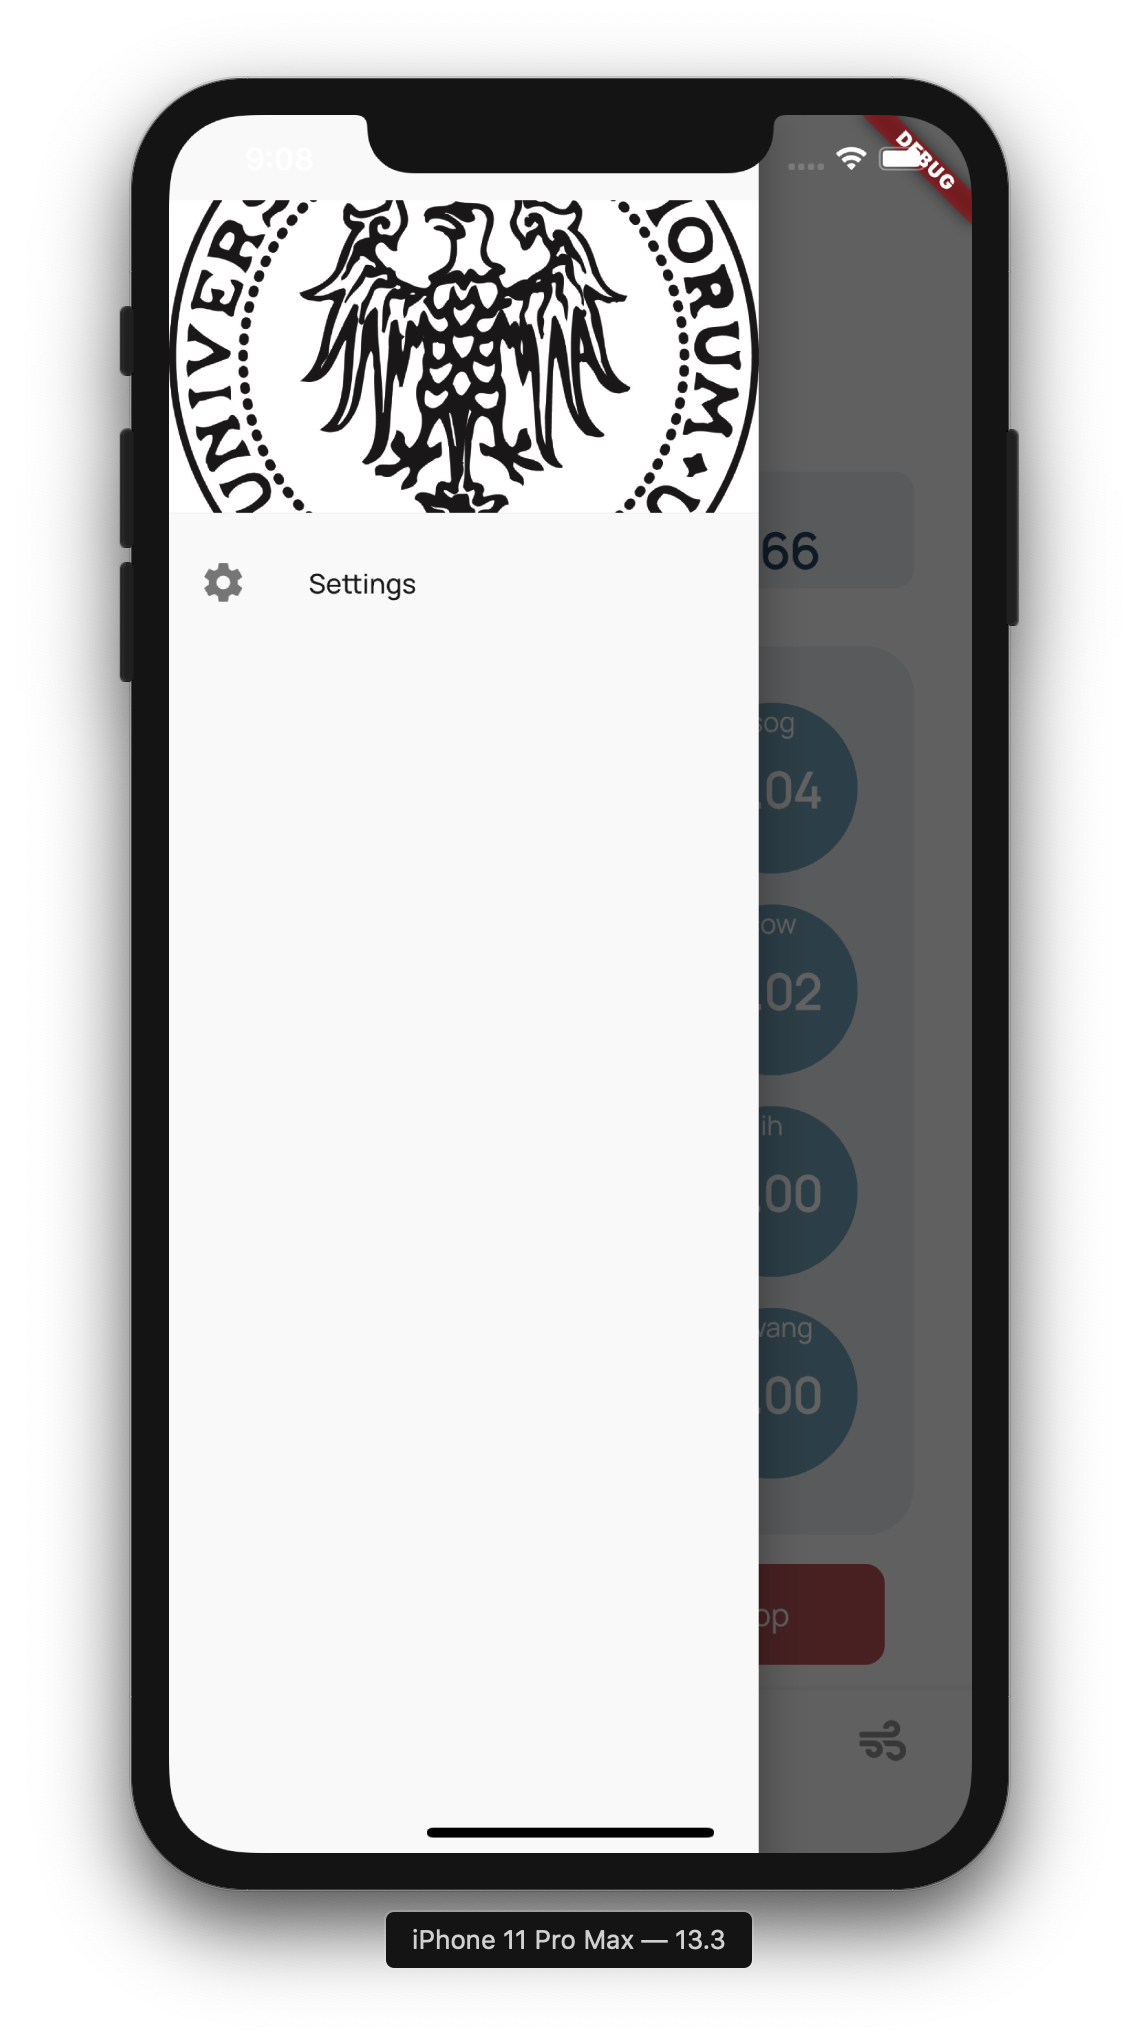
\includegraphics[scale=0.34]{drawer}
	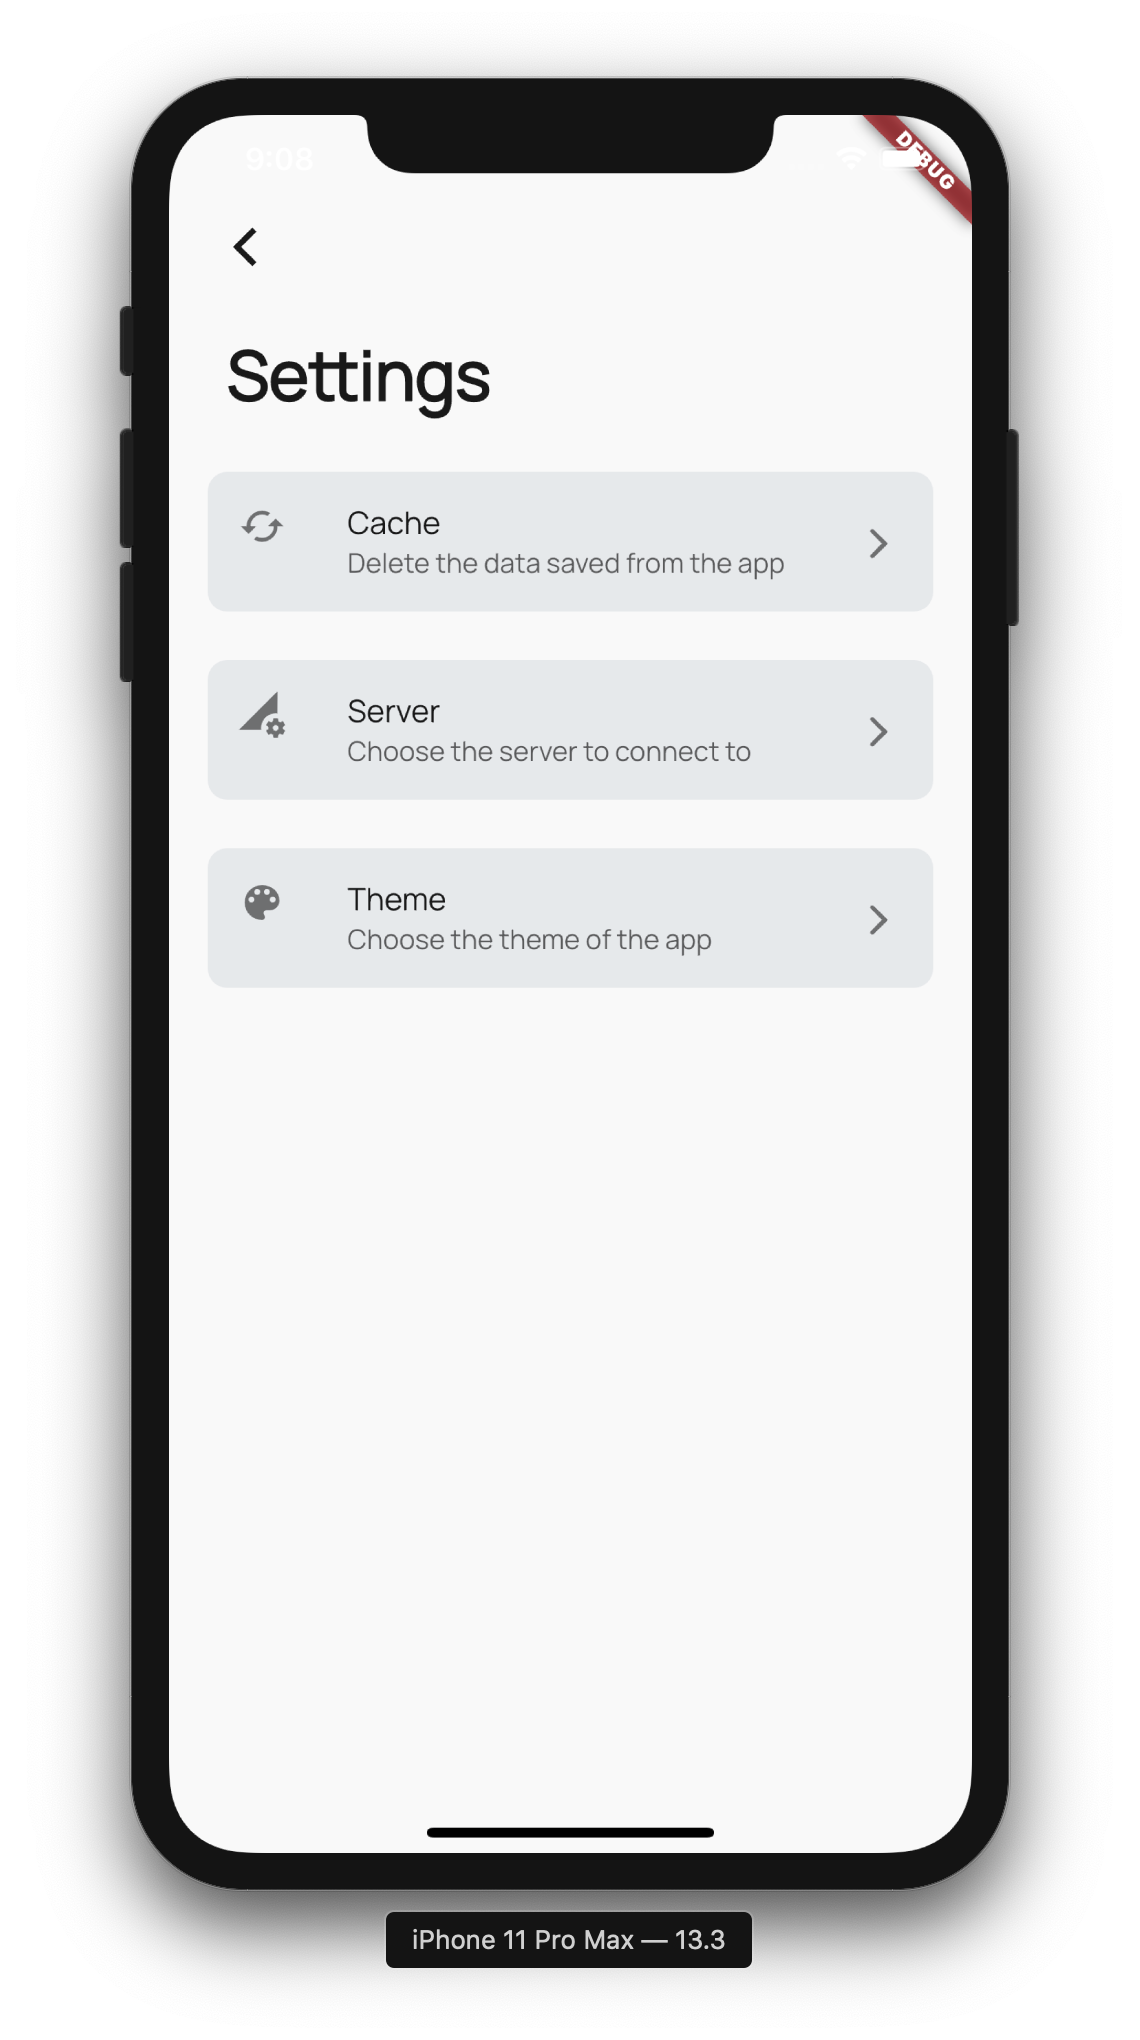
\includegraphics[scale=0.34]{settings}
	\caption[Screenshot - Drawer e della schermata Settings]{Screenshot del \textit{drawer} dell'applicazione (a sinistra) e della schermata di \textit{Settings} (a destra).}\label{xyz}
\end{figure}

\newpage

\subsubsection{Cache}
In questa schermata l'utente può eliminare i dati salvati nella \textit{cache}. Facendo un \textit{tap} sull'unica voce presente nella schermata (Figura 6.11), si presenterà un \textit{Alert Dialog} per chiedere la conferma della pulizia della cache. Se la cache è vuota, anche se si volesse selezionare la voce, non comparirà alcuna Alert Dialog.

\begin{figure}
	\begin{center}
		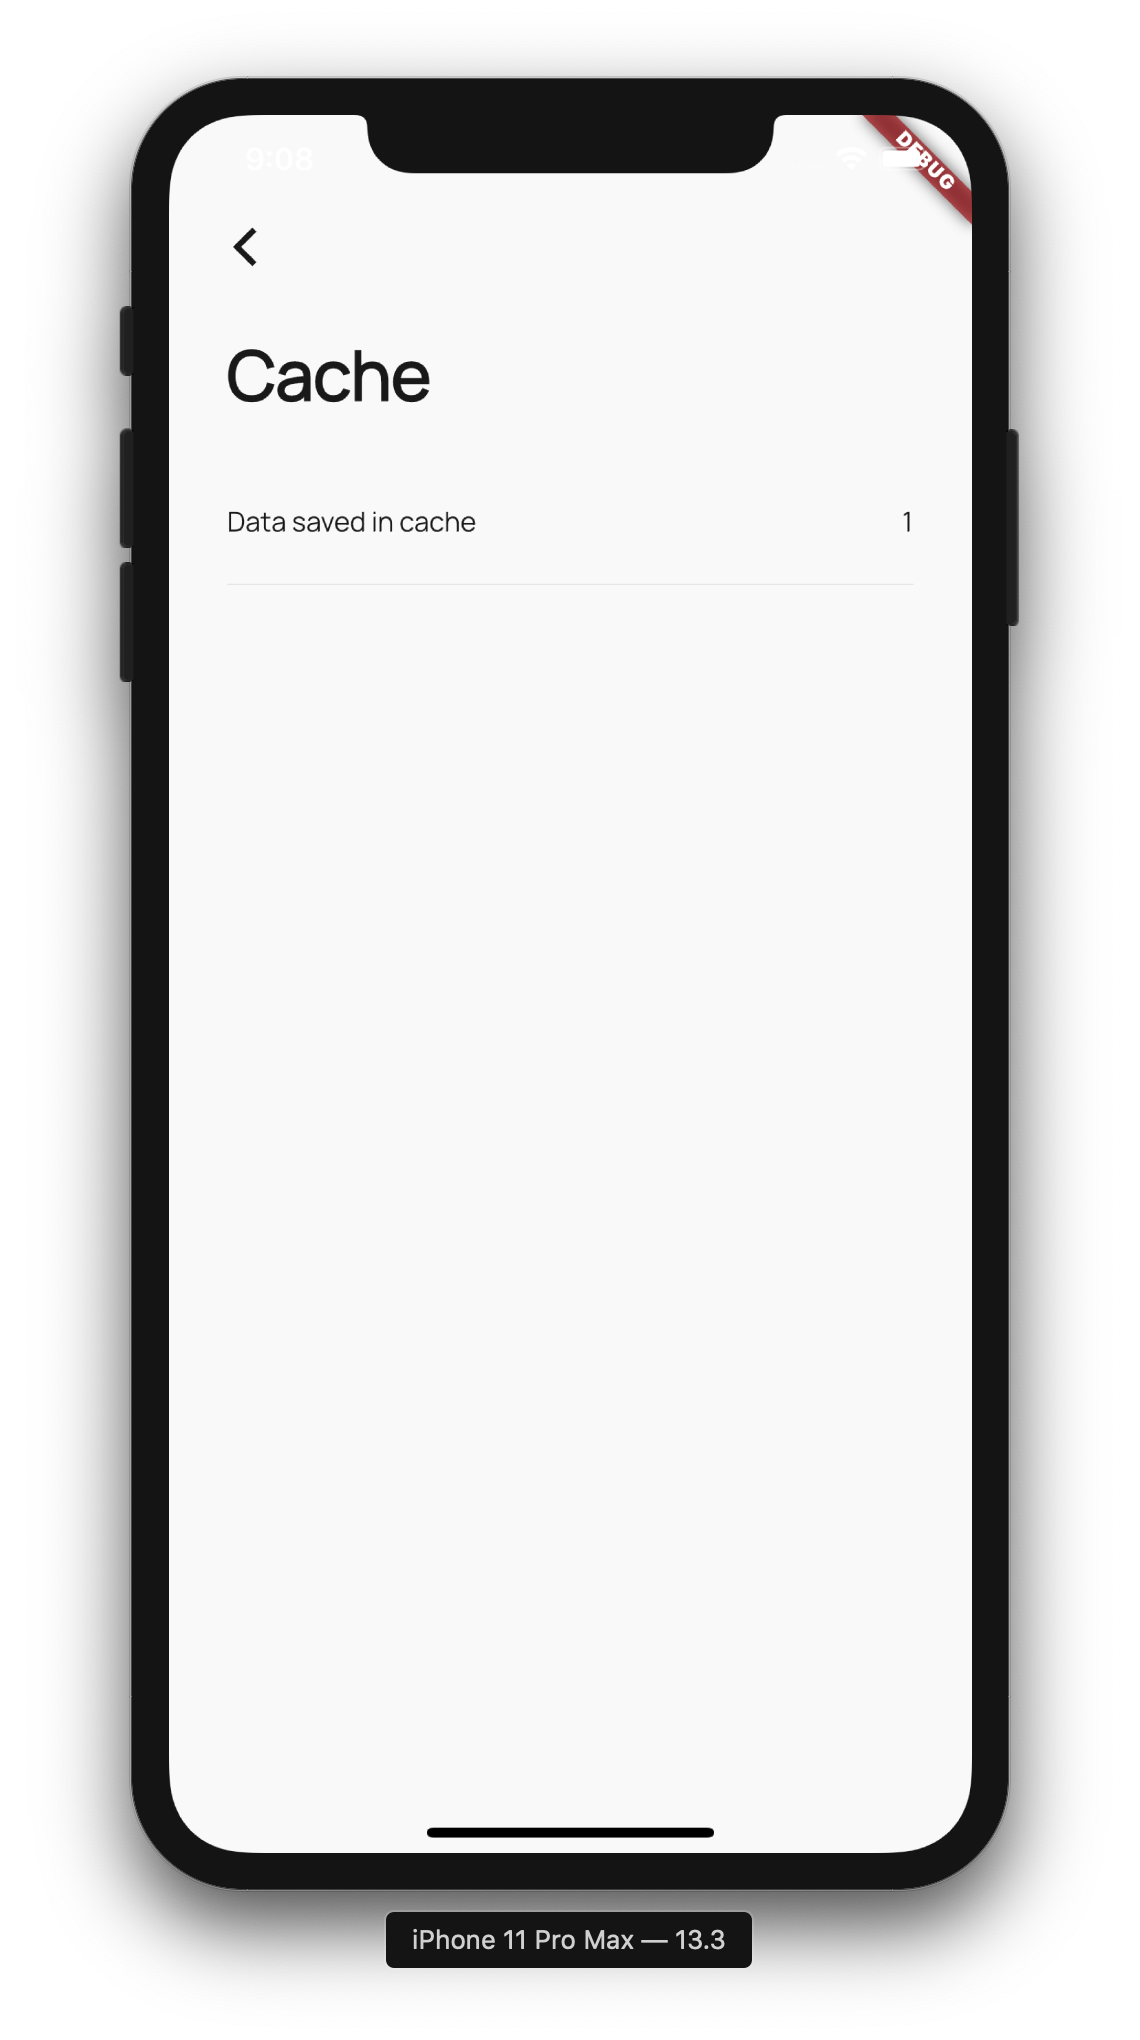
\includegraphics[scale=0.34]{cache}
		\caption[Screenshot - Cache]{Screenshot della schermata \textit{Cache}.}
		\label{figura:cache}
	\end{center}
\end{figure}

Dagli screenshot in Figura 6.12, è possibile notare che sono state riprodotte le Alert Dialog sia per i dispositivi con sistema operativo Android che iOS. Le diverse Alert Dialog sono fornite direttamente da Flutter.

\begin{figure}[htp]
	\centering
	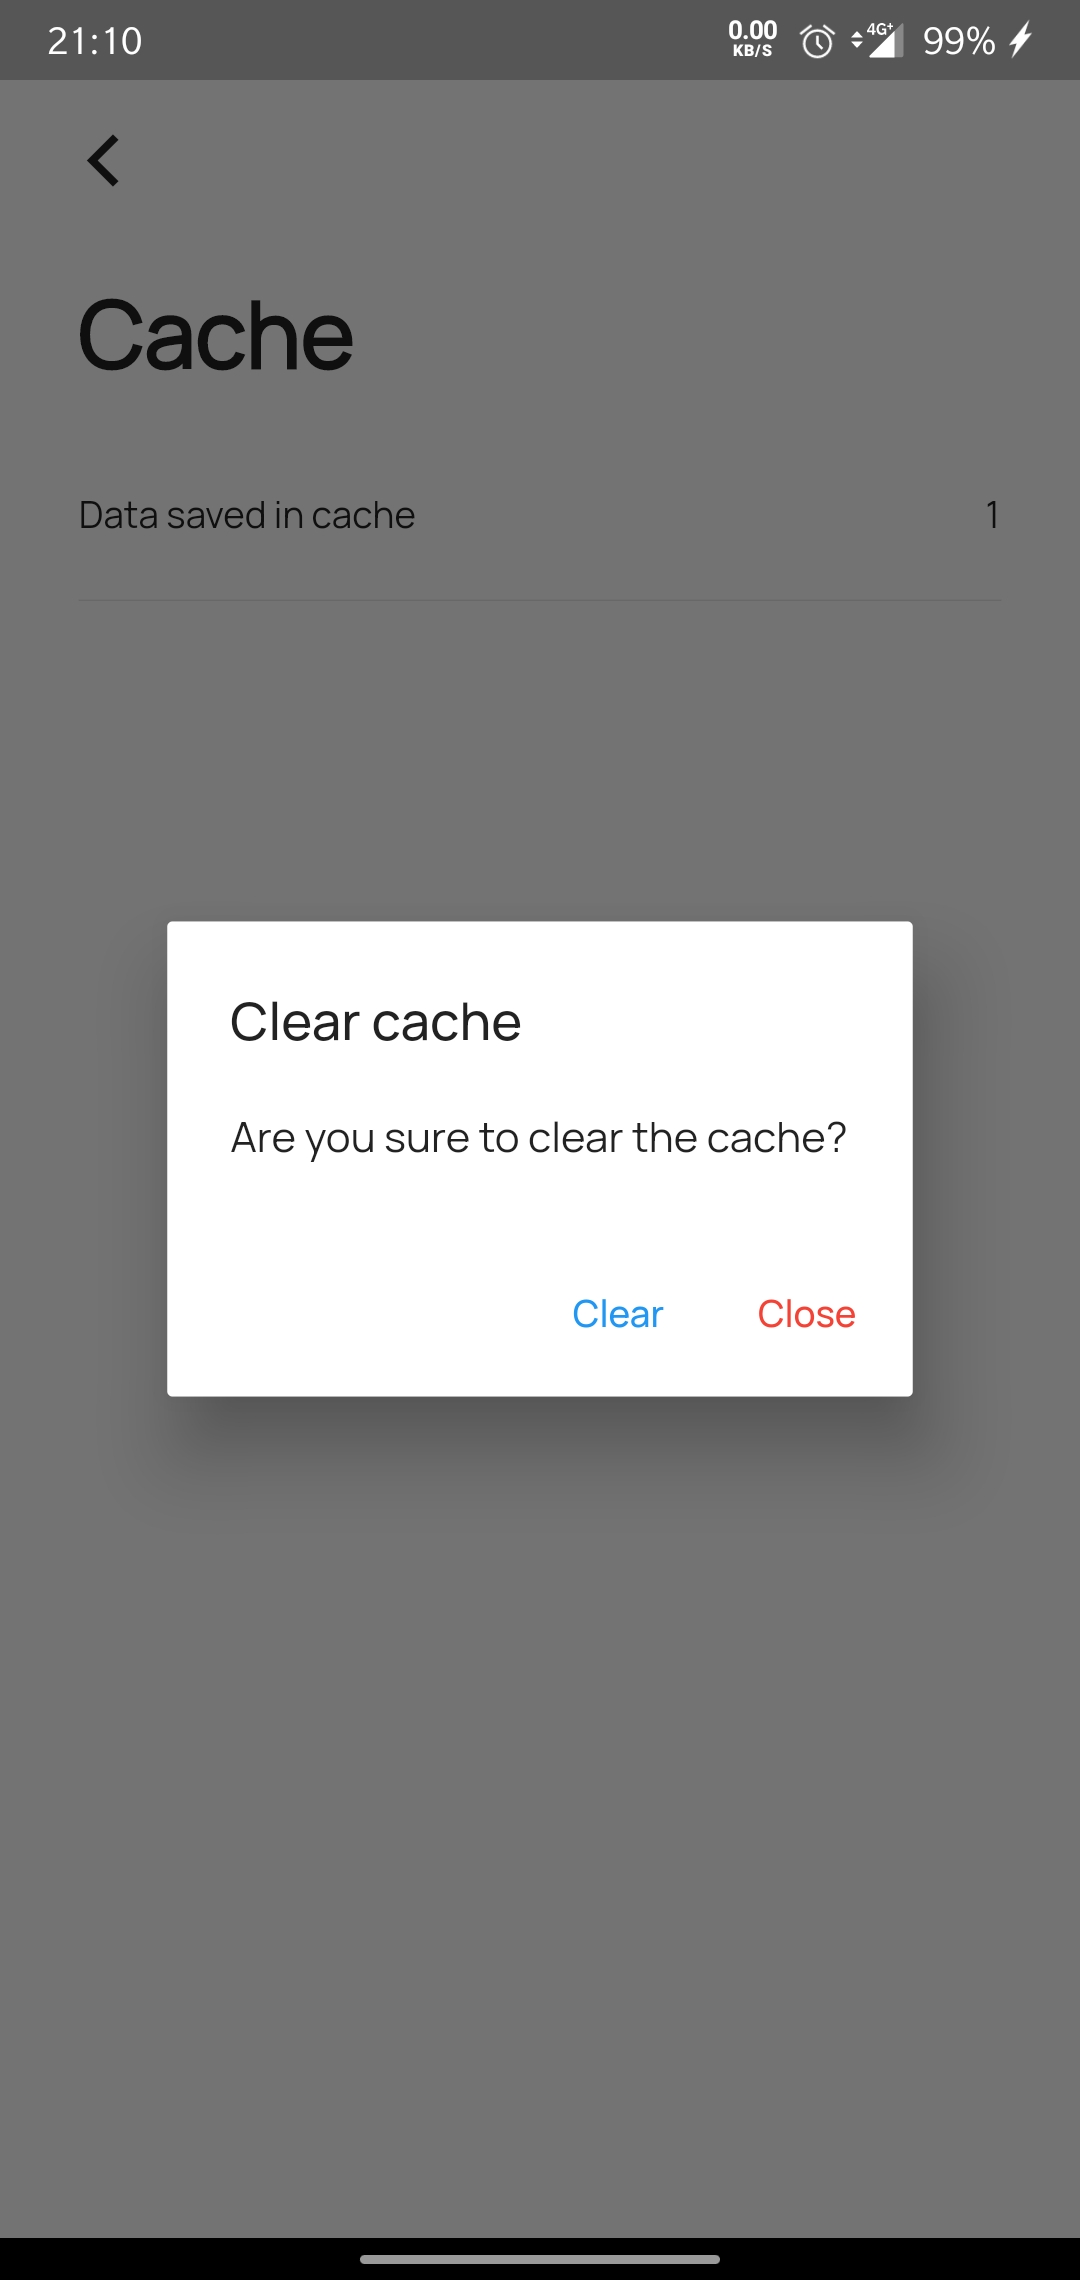
\includegraphics[scale=0.15]{cache_android_dialog}
	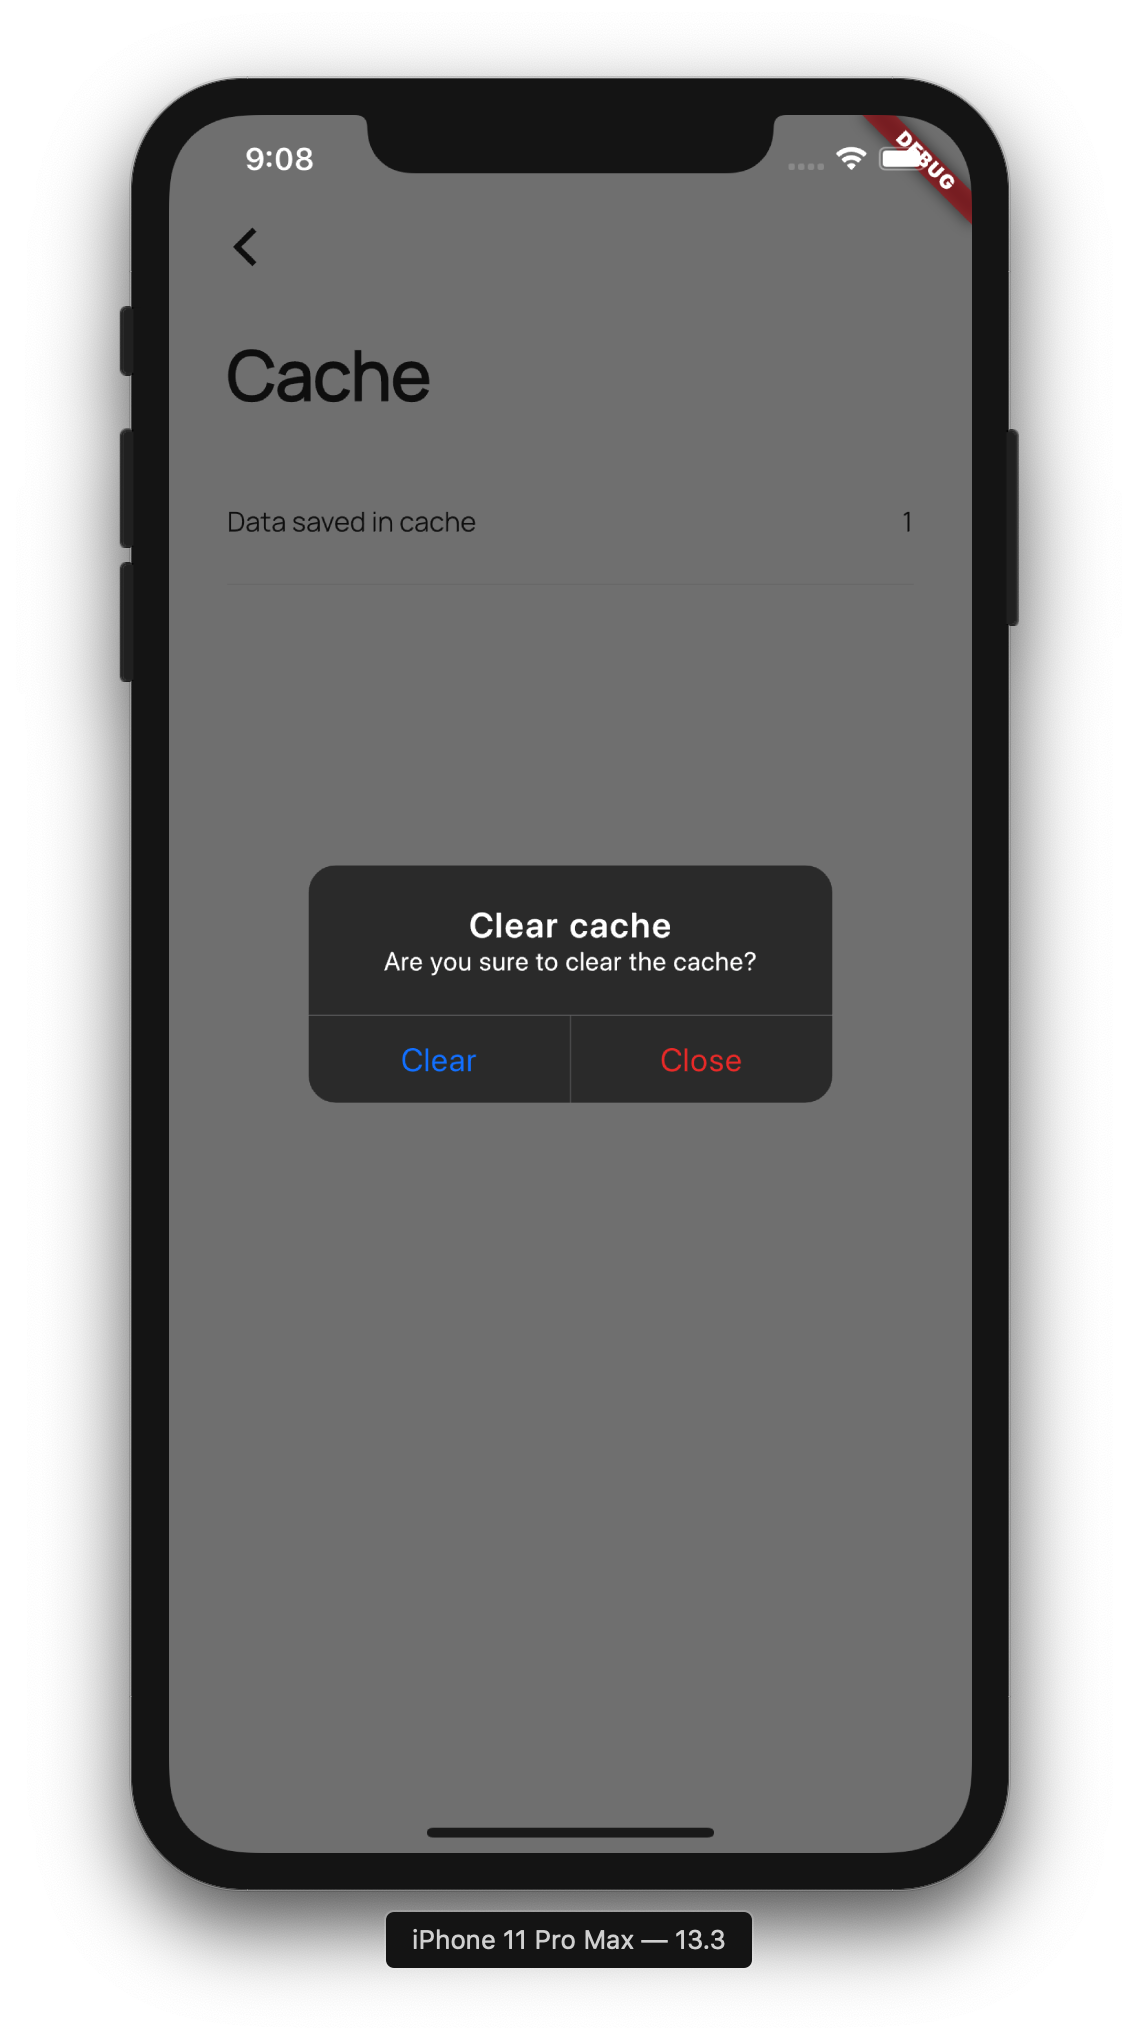
\includegraphics[scale=0.35]{cache_ios_dialog}
	\caption[Screenshot - Alert Dialog in Android e iOS della schermata Cache]{Screenshot dell'\textit{Alert Dialog} per dispositivi Android (a sinistra) e iOS (a destra).}\label{xyz}
\end{figure}

\newpage

\subsubsection{Server}
Questa schermata offre due principali funzionalità:
\begin{enumerate}
	\item Controllo dello stato della \textit{connessione};
	\item Modifica dei parametri per la connessione al server e per il \textit{polling}.
\end{enumerate}

\begin{figure}
	\begin{center}
		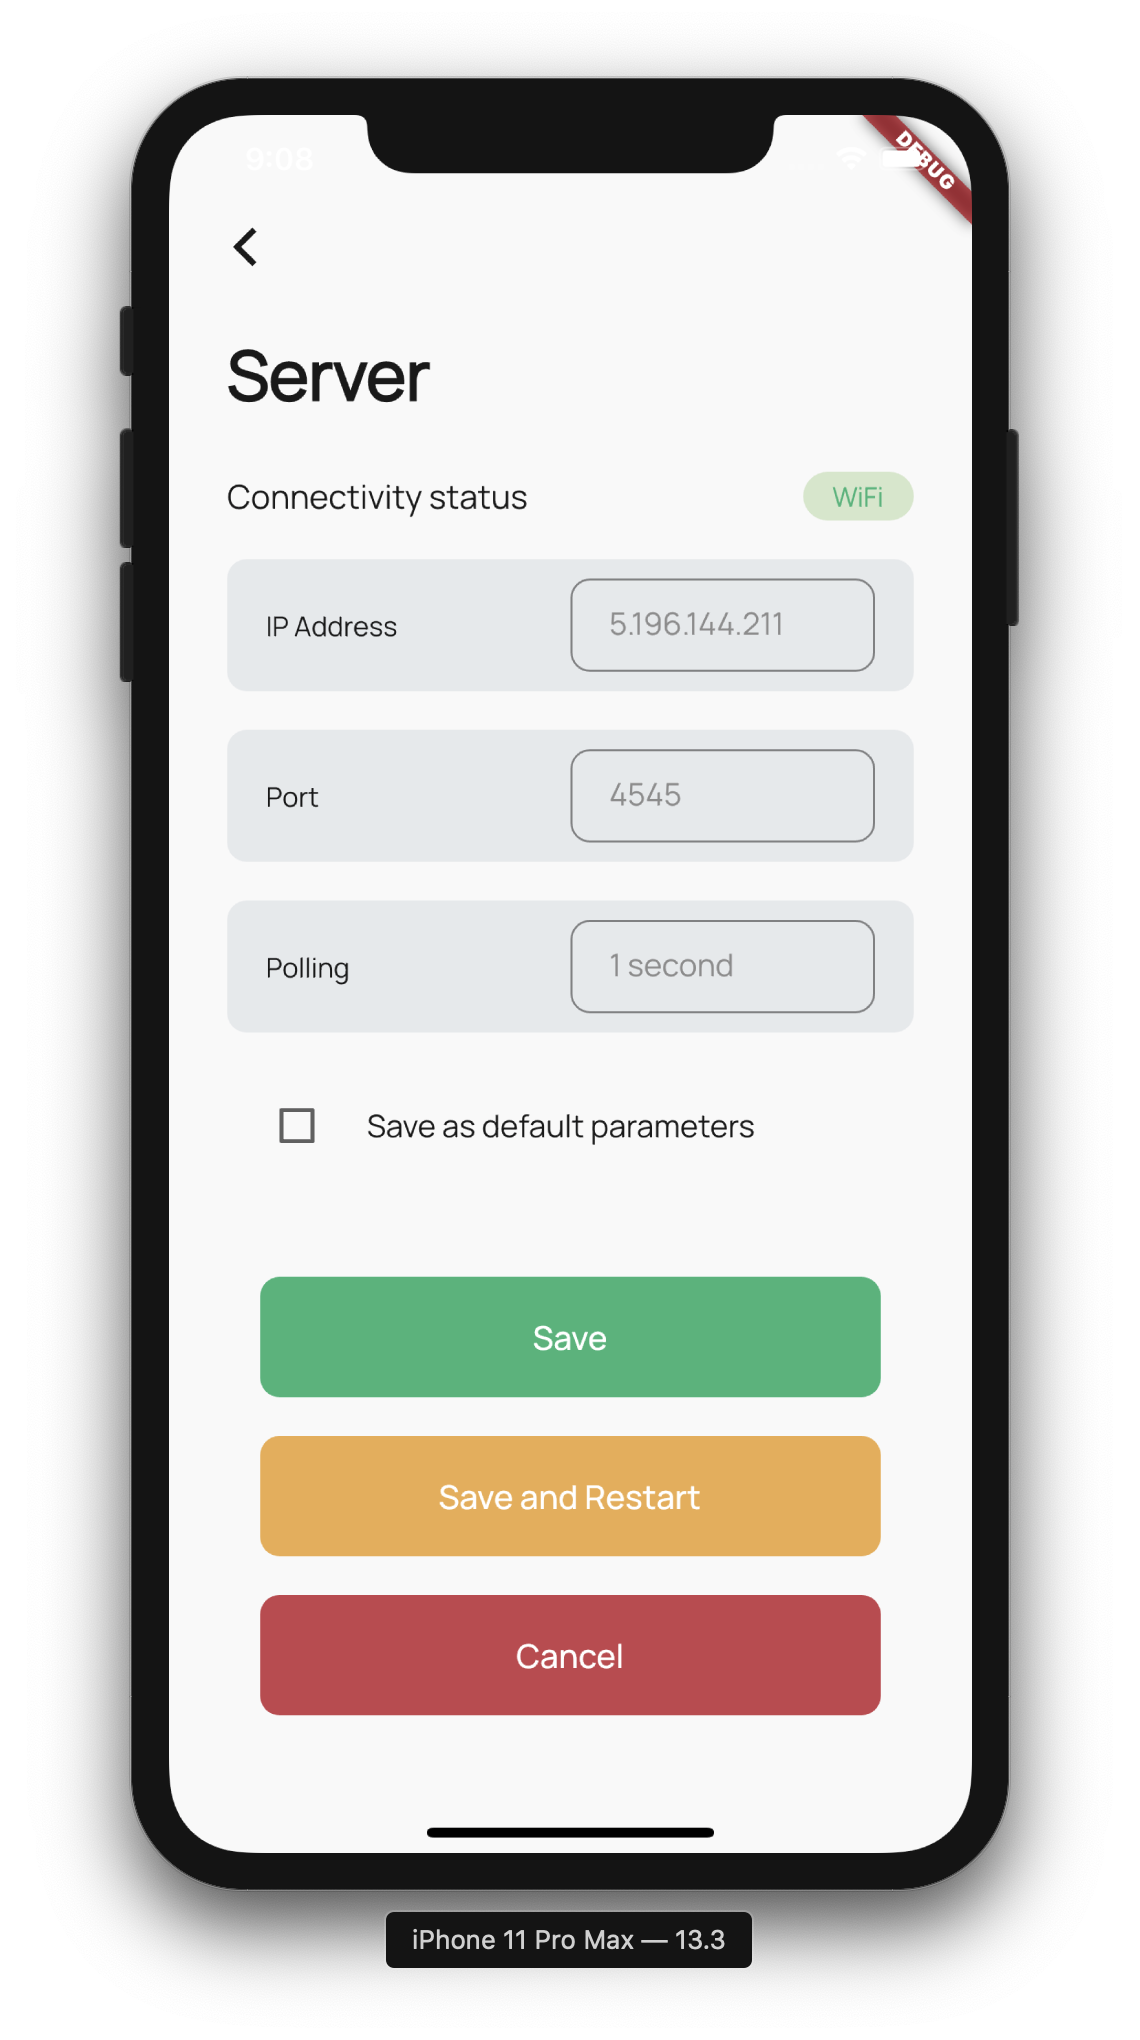
\includegraphics[scale=0.34]{server}
		\caption[Screenshot - Server]{Screenshot della schermata \textit{Server}.}
		\label{figura:server}
	\end{center}
\end{figure}

Per quanto riguarda la prima funzionalità, quando viene rilevato un cambio di stato della connessione, ad esempio da una rete \textit{WiFi} ad una rete \textit{mobile}, questo viene reso noto dalla componente grafica evidenziata negli screenshot presenti nella Figura 6.14. Nel caso in cui sia assente la connessione ad Internet, viene mostrata la dicitura "\textit{offline}". Questa funzionalità è stata possibile implementarla grazie all'utilizzo di un particolare plugin che offre il team di Flutter: \verb|connectivity| (l'applicazione si basa sulla versione \verb|0.4.8+2| del plugin) \cite{connectivity_plugin}. Questo pacchetto fornisce una serie di metodi che permettono di controllare lo stato della connessione.

\begin{figure}[htp]
	\centering
	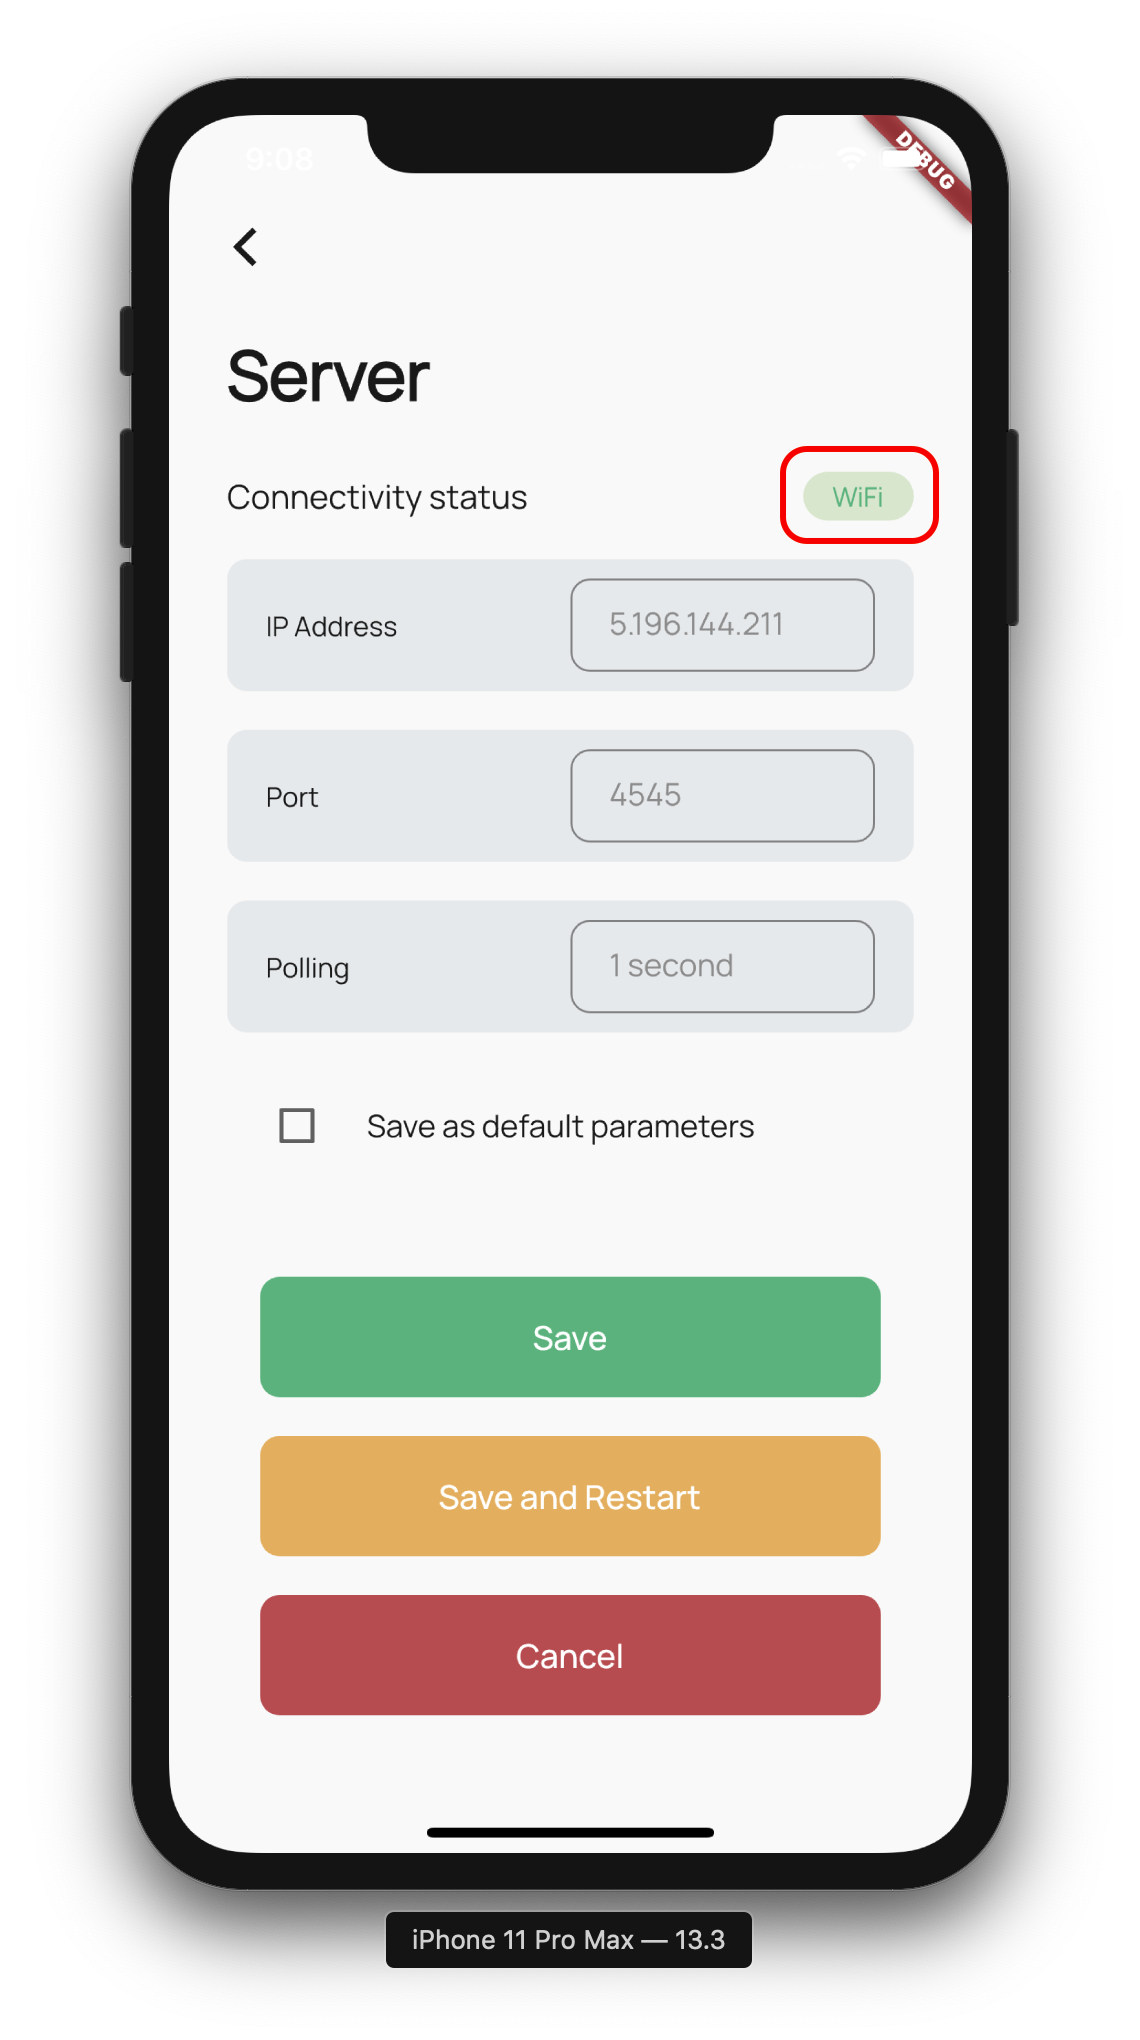
\includegraphics[scale=0.34]{server_online_status}
	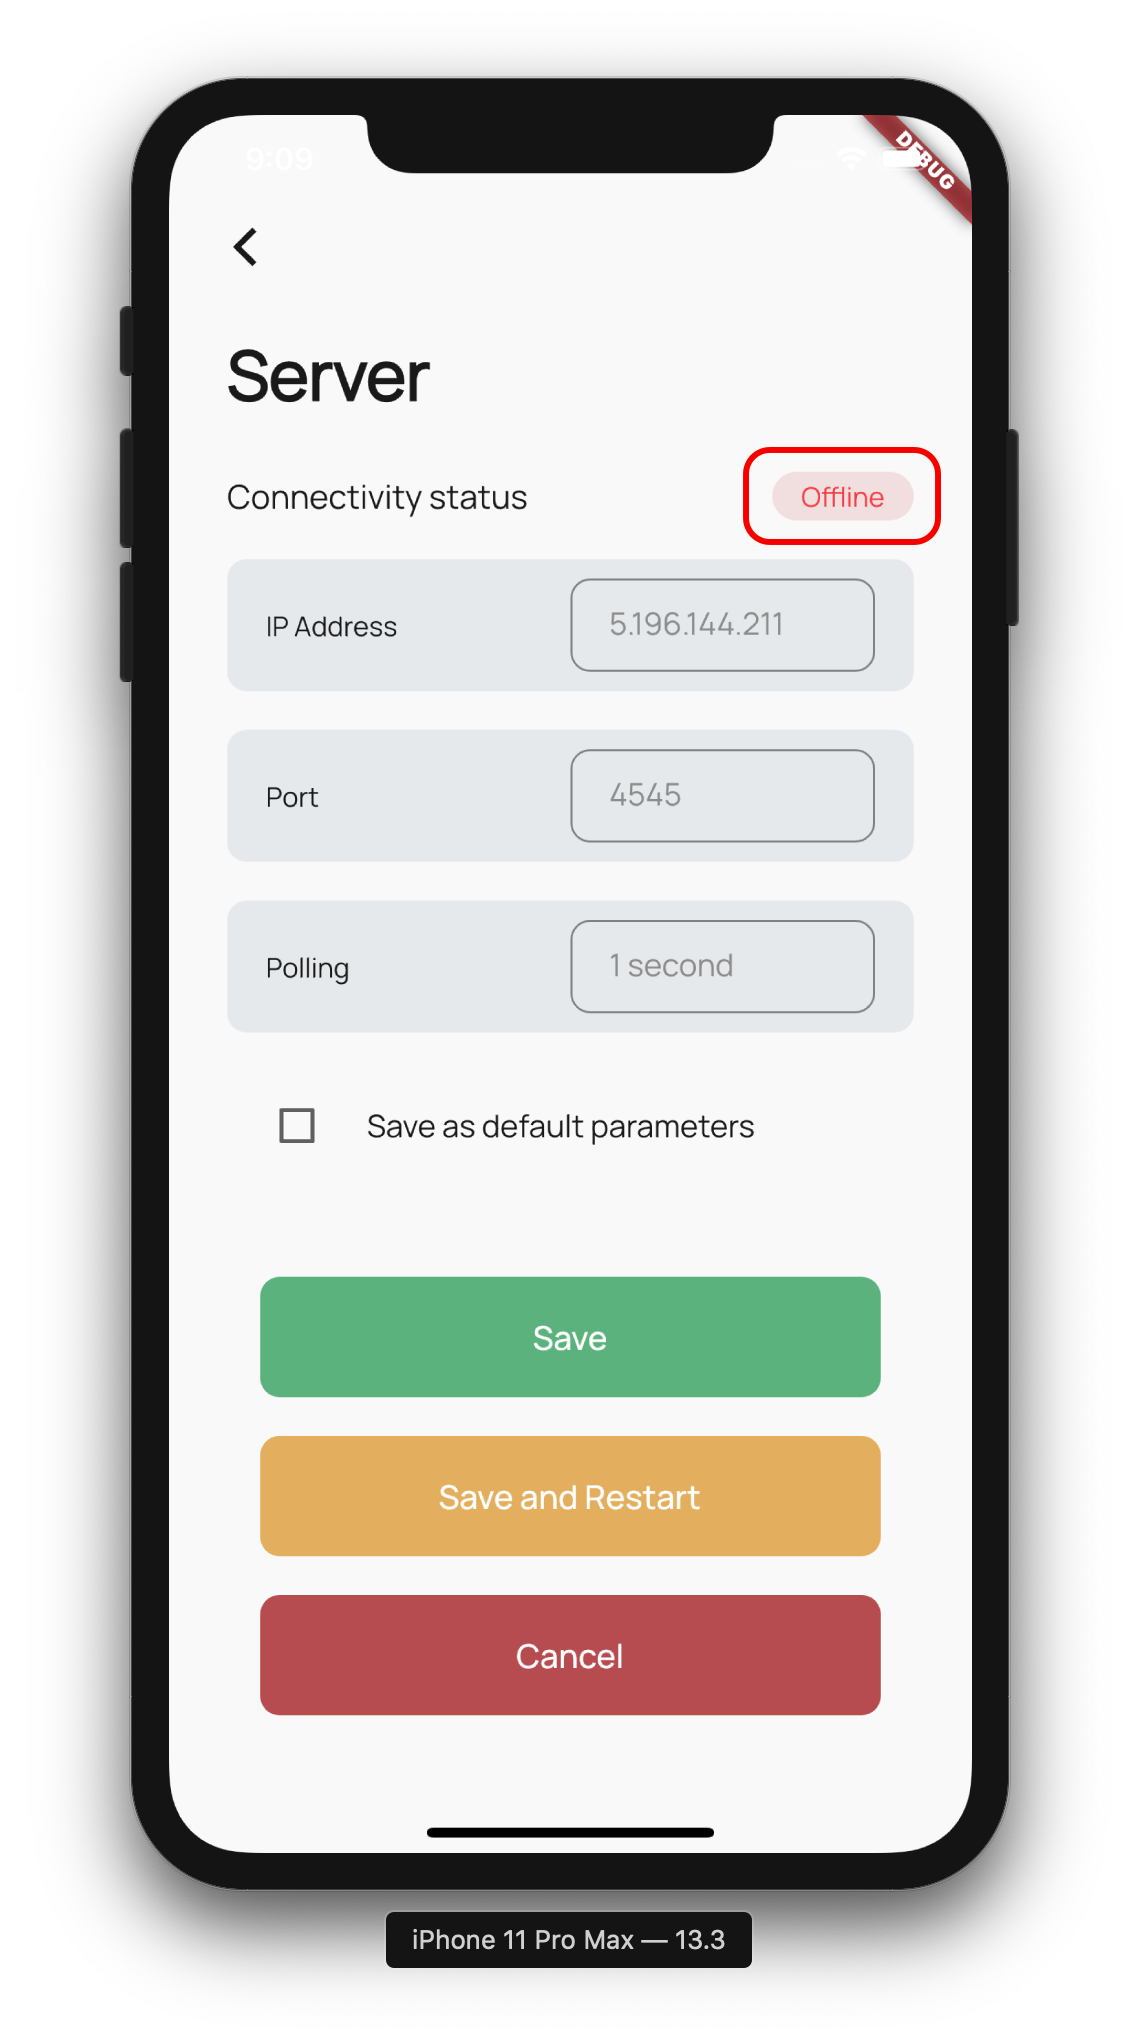
\includegraphics[scale=0.34]{server_offline_status}
	\caption[Screenshot - Controllo dello stato della connessione nella schermata Server]{Tramite un apposito ascoltatore ed il pacchetto (\textit{connectivity 0.4.8+2} \cite{connectivity_plugin}), l'utente può verificare lo stato della connessione Internet.}\label{xyz}
\end{figure}

Dalla riga 8 fino alla riga 15, viene inizializzato un ascoltatore che appena rileva un cambio di stato della connessione, aggiorna lo stato dell'applicazione (nel metodo \verb|setState(() {})|). In questo pezzo di codice, viene sfruttata appieno la \textit{programmazione reattiva}: appena il contenuto della variabile privata \verb|_connectivityStatus| cambia, questo viene propagato nell'albero dei Widget, senza dover eseguire ulteriori istruzioni. 

\newpage

\begin{lstlisting}
...

@override
  void initState() {
    super.initState();
    getInitialStatus();

    _subscription = Connectivity()
        .onConnectivityChanged
        .listen((ConnectivityResult result) {
      setState(() {
        _connectivityStatus = getTextStatus(result);
      });
    });
  }

  void getInitialStatus() async {
    var connectivityResult = await (
    Connectivity().checkConnectivity());
    setState(() {
      _connectivityStatus = getTextStatus(connectivityResult);
    });
    
...
\end{lstlisting}

Per quanto riguarda la funzionalità di modifica dei parametri, quando i dati inseriti rispettano i formati e i vincoli richiesti, è possibile notare nella parte inferiore dell'applicazione una \textit{SnackBar}. Lo scopo della \textit{SnackBar} è quello di notificare l'utente che i dati sono stati inseriti correttamente e che l'aggiornamento dei nuovi parametri inseriti è avvenuto con successo (Figura 6.15). Nel caso in cui invece l'utente abbia inserito dei dati non corretti dal punto di vista del formato o dei vincoli imposti, viene visualizzata una \textit{Alert Dialog} (Figura 6.16). Se vengono generati più errori in un'unica richiesta, questi verranno mostrati tutti insieme in una sola \textit{Alert Dialog}.
\begin{figure}
	\begin{center}
		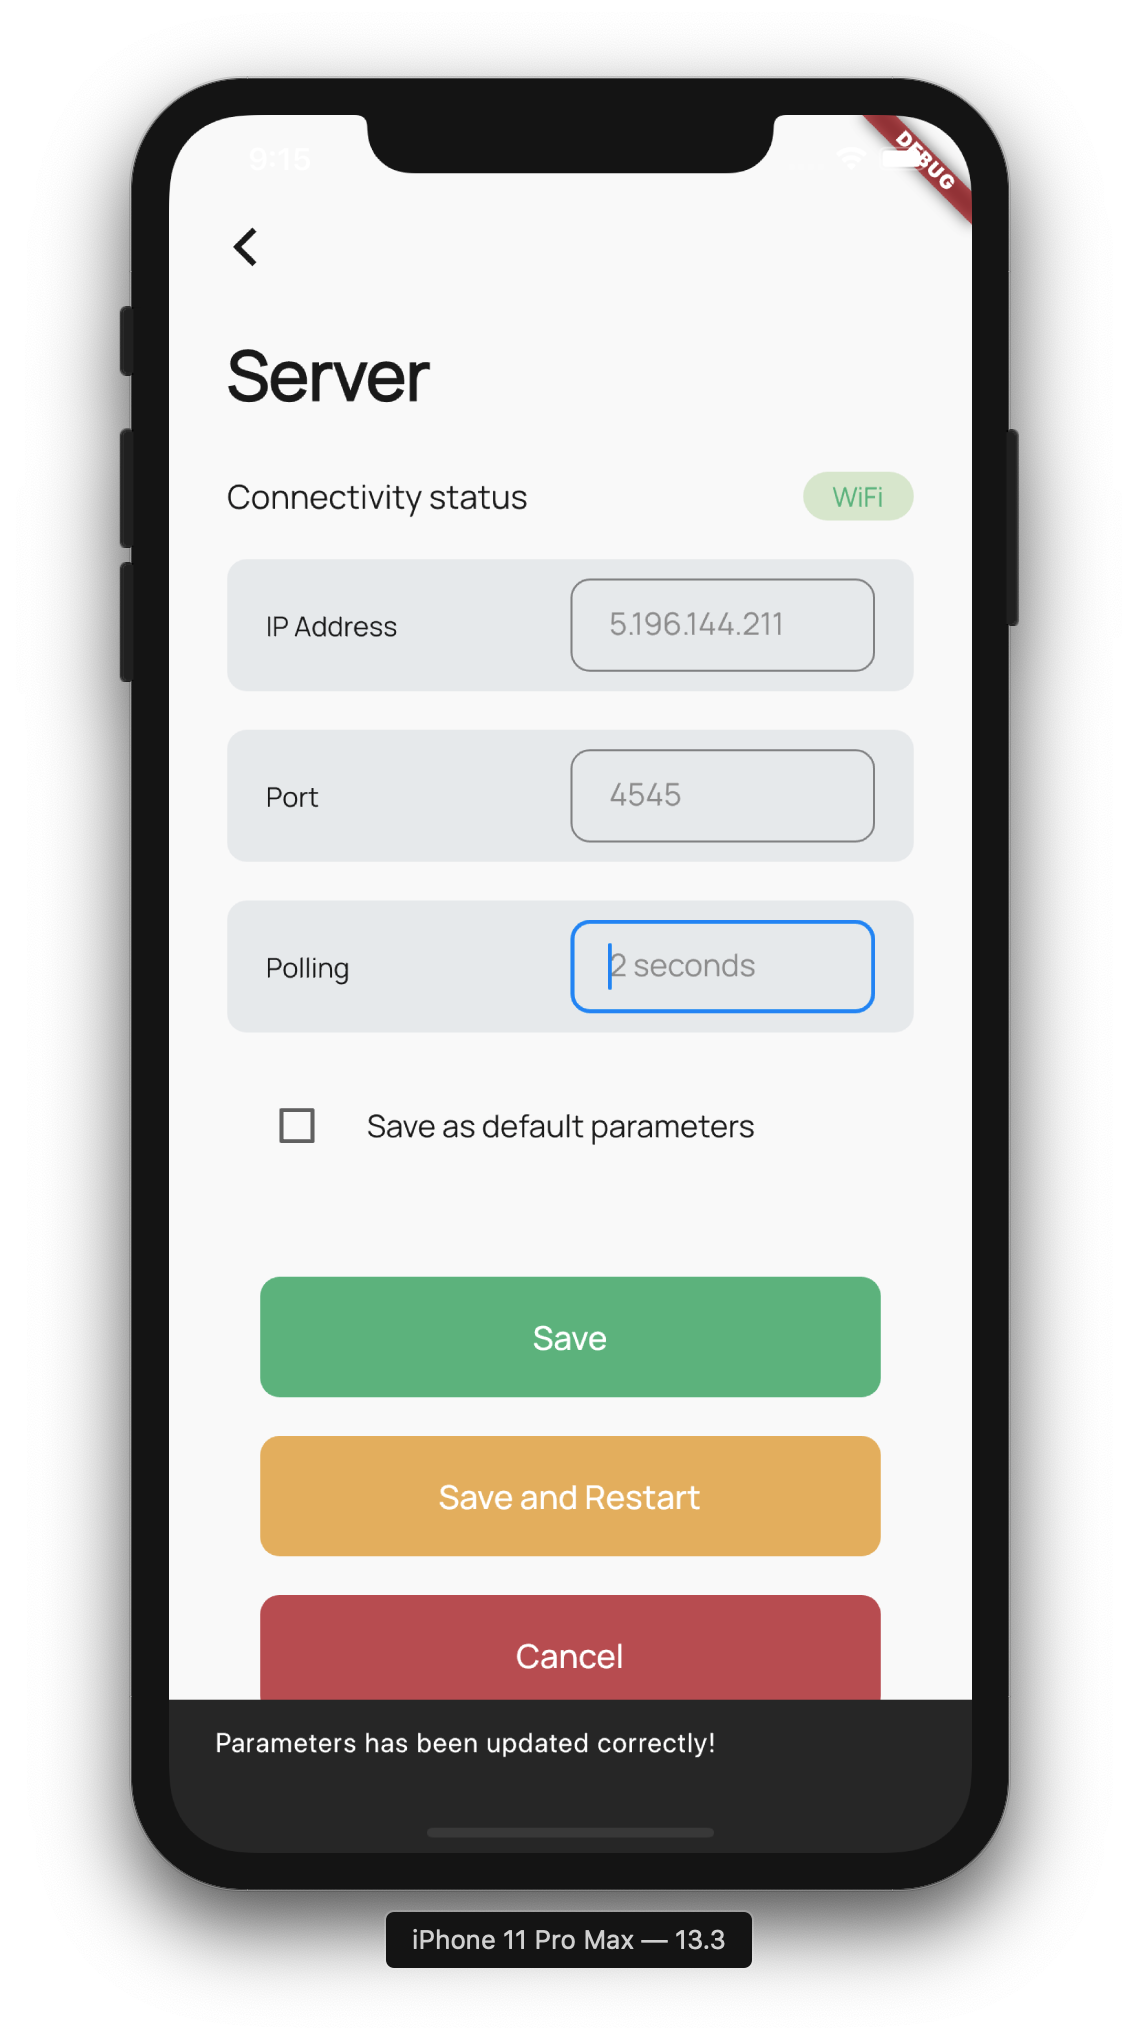
\includegraphics[scale=0.34]{server_successful}
		\caption[Screenshot - Salvataggio dei dati con successo nella schermata Server]{È possibile notare la \textit{SnackBar} che notifica che i dati sono stati inseriti correttamente e che sono stati aggiornati.}
		\label{figura:server_successful}
	\end{center}
\end{figure}

\begin{figure}[htp]
	\centering
	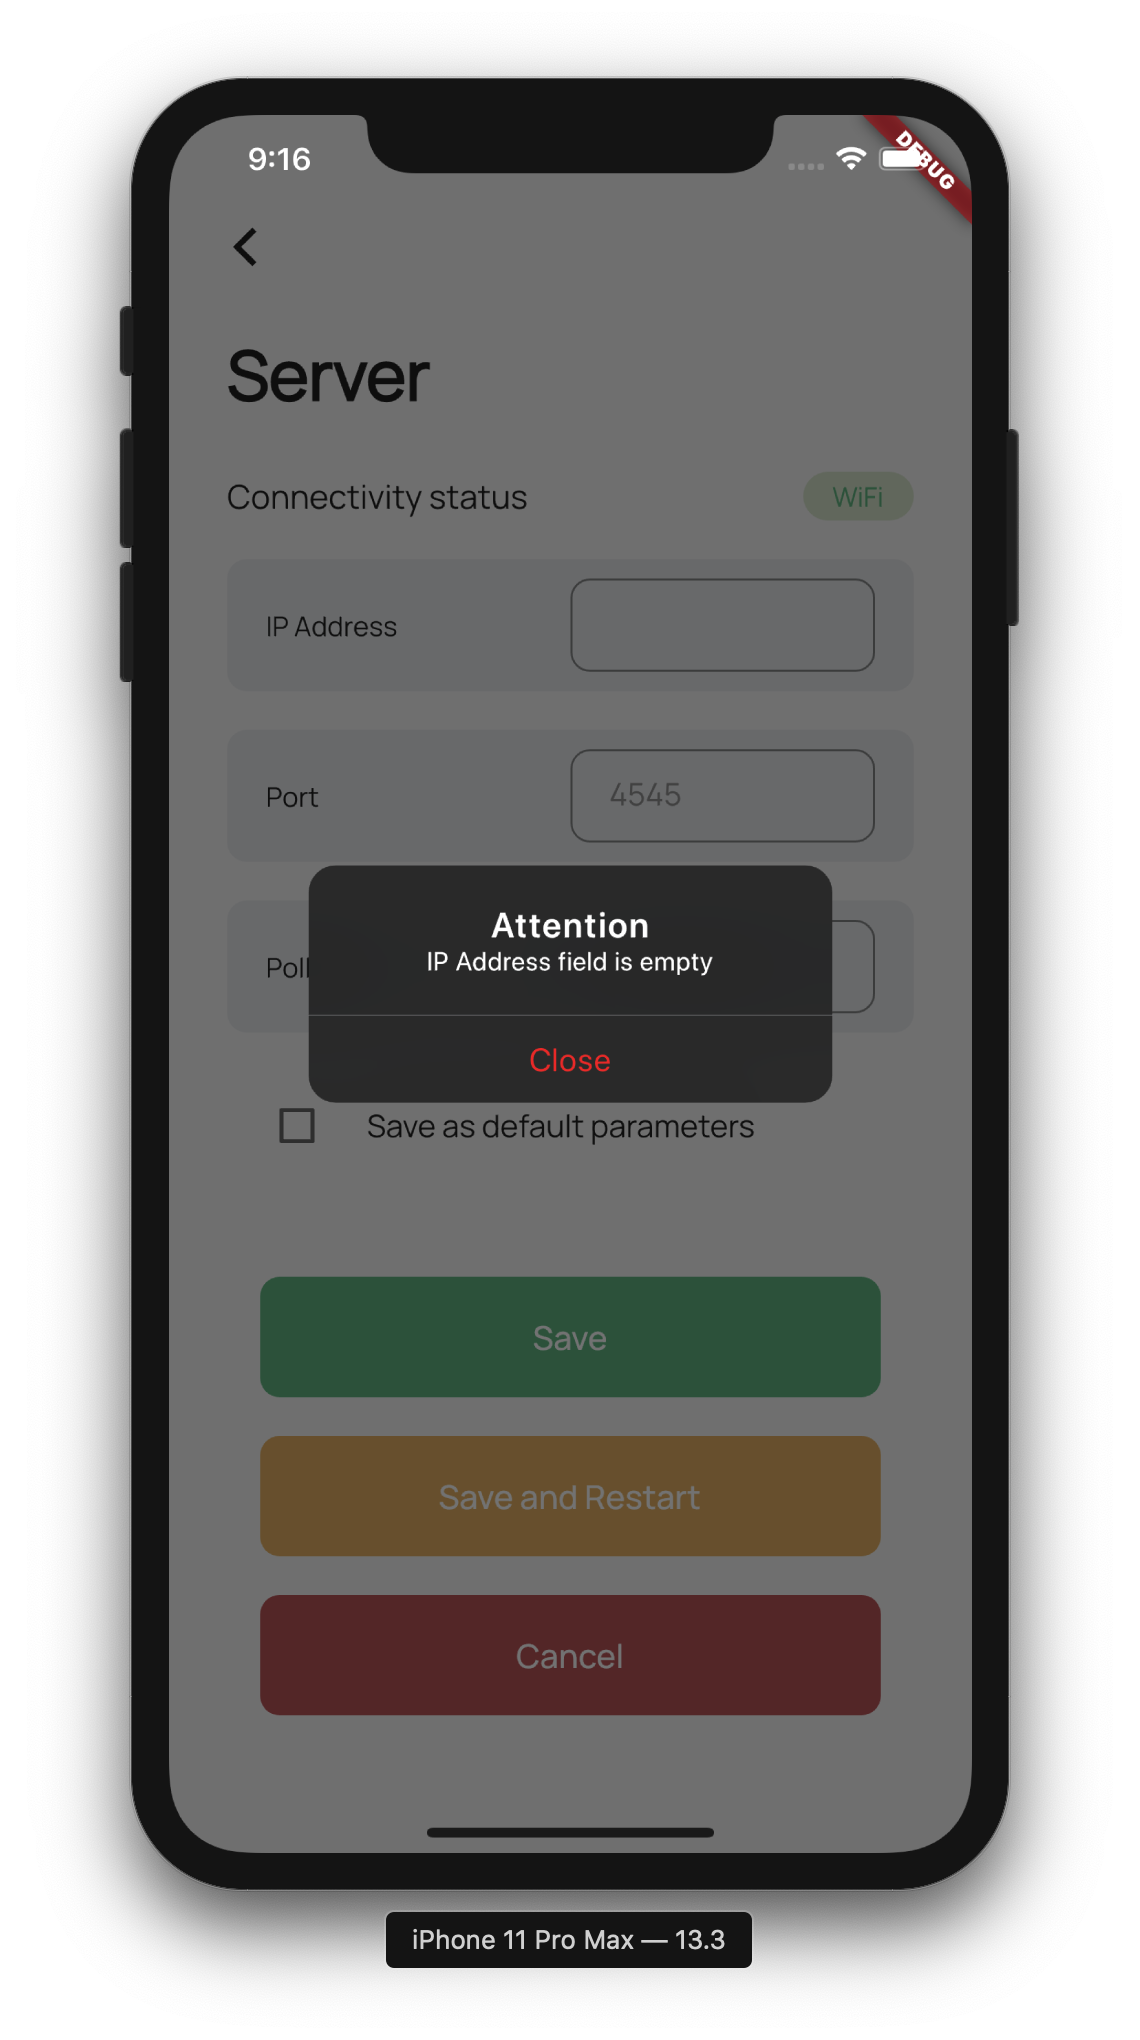
\includegraphics[scale=0.34]{server_error}
	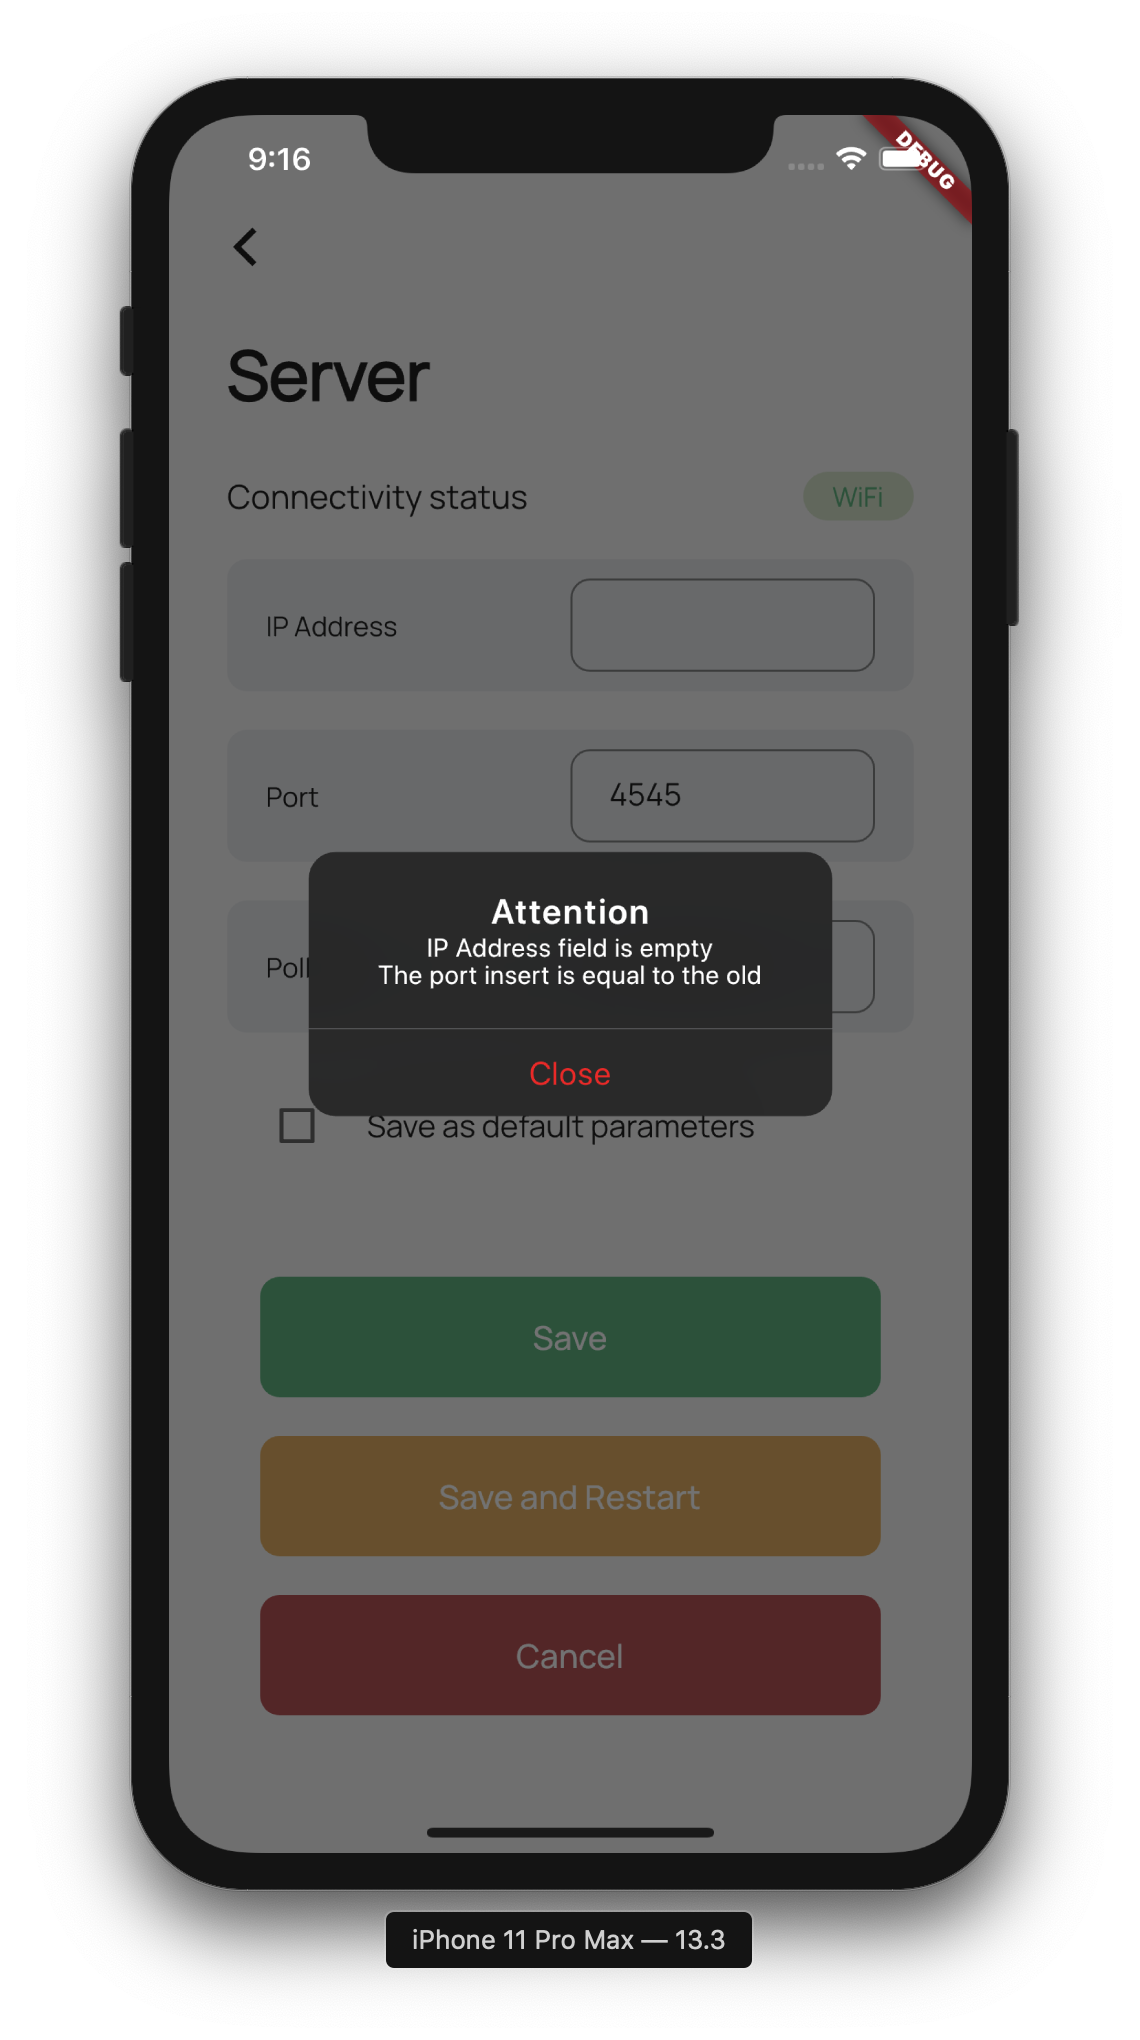
\includegraphics[scale=0.34]{server_errors}
	\caption[Screenshot - Alert Dialog di errore nella schermata Server]{Quando vengono inseriti dei parametri in un formato non accettato, viene visualizzata una \textit{Alert Dialog}.}\label{xyz}
\end{figure}

\newpage

\subsubsection{Temi}
In questa schermata, l'utente può selezionare uno dei temi forniti dall'applicazione. In questa versione dell'app sono presenti soltanto due temi: \textit{default} e ad \textit{alto contrasto}.
È possibile attivare o disattivare l'attivazione del tema ad \textit{alto contrasto} tramite l'apposito \textit{switch} (Widget \verb|Switch|). Quando il tema viene attivato o disattivato, anche il testo dell'opzione cambia. Osservando la Figura 6.17, nella schermata di sinistra il tema ad \textit{alto contrasto} è attivato, mentre a destra è disattivato.

\begin{figure}[htp]
	\centering
	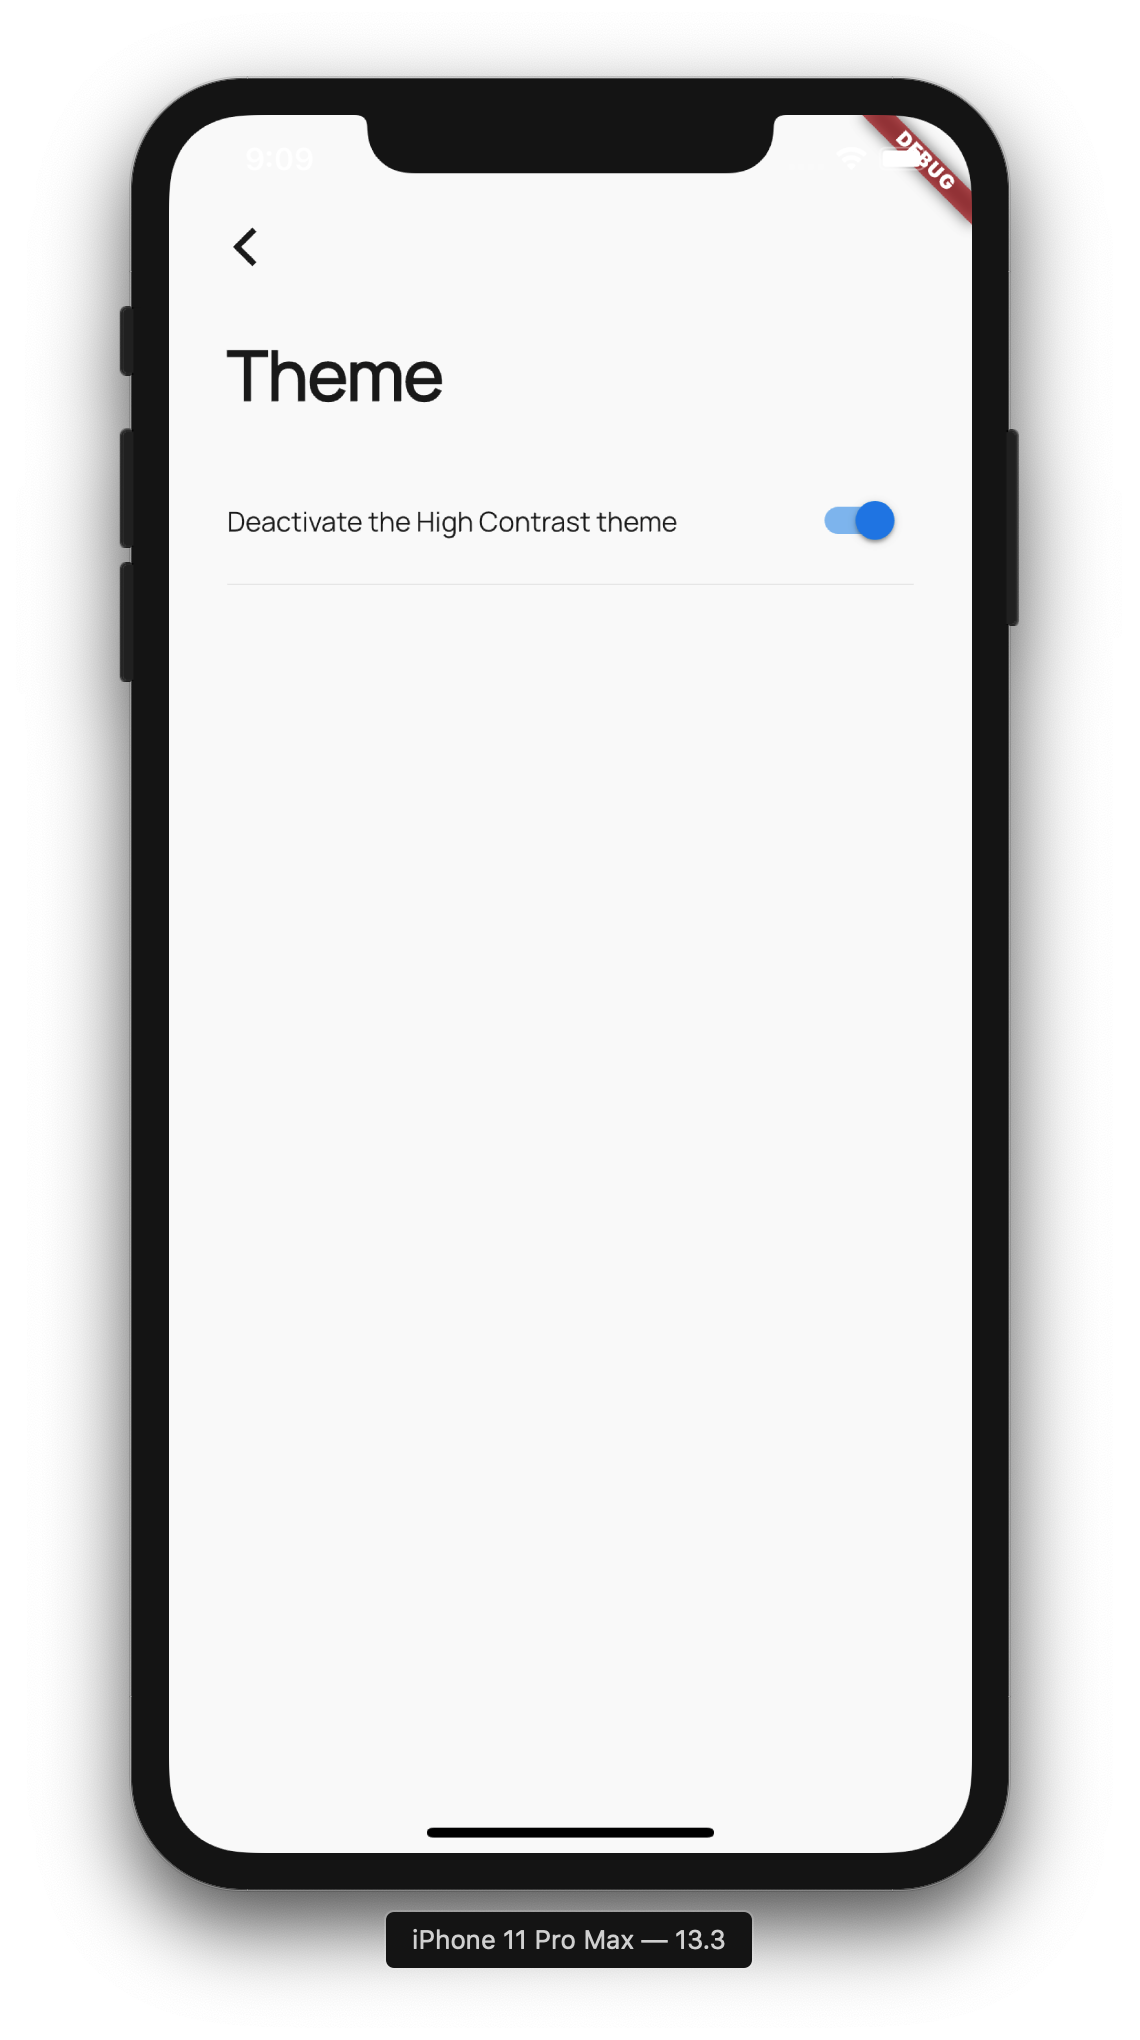
\includegraphics[scale=0.34]{theme_high_contrast_activate}
	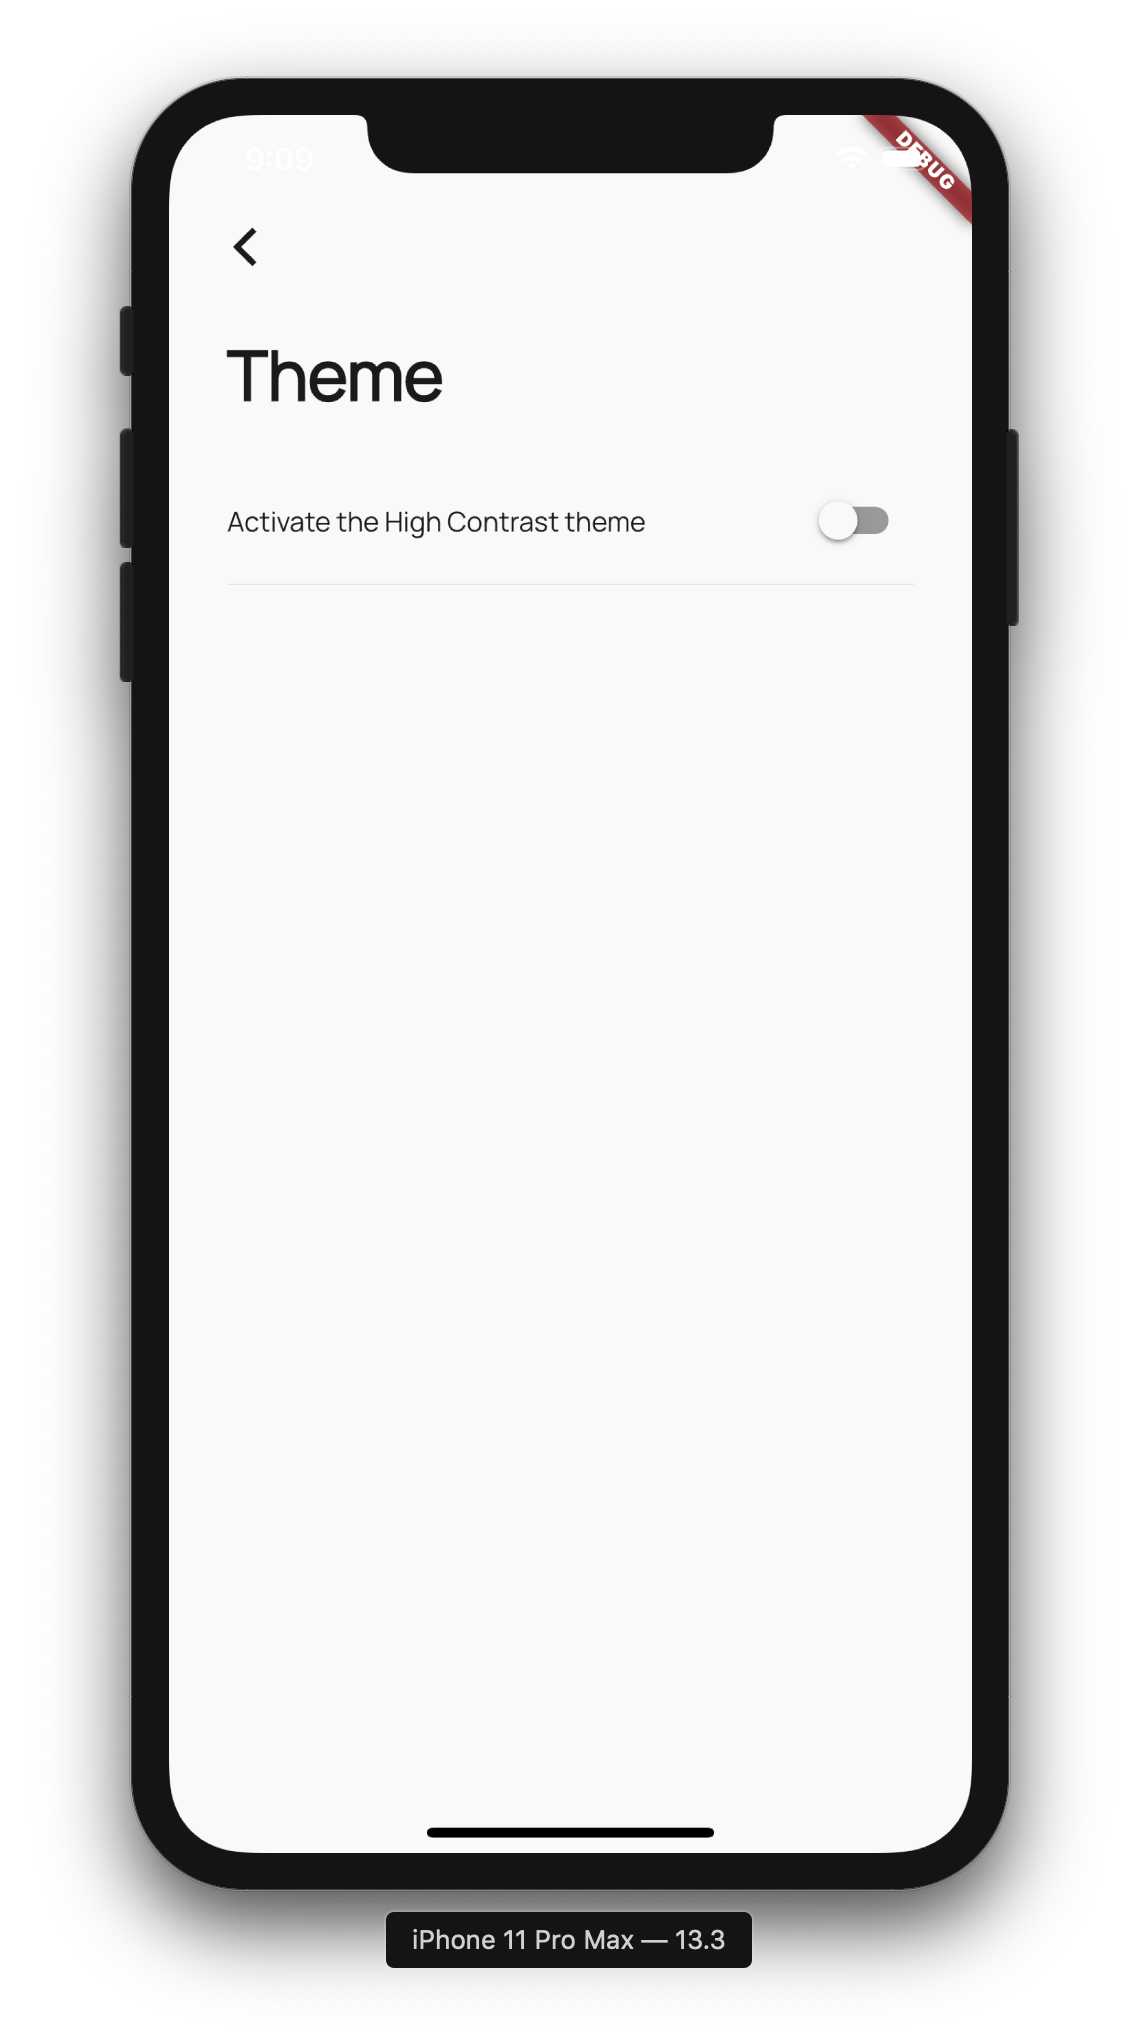
\includegraphics[scale=0.34]{theme_high_contrast_deactivate}
	\caption[Screenshot - Schermata per la scelta del tema]{Screenshot della schermata \textit{Theme}.}\label{xyz}
\end{figure}

È possibile vedere dagli screenshot in Figura 6.18, come si presenta l'applicazione con il tema ad \textit{alto contrasto} attivato. Le schermate \textit{GPS} e \textit{Wind} hanno il medesimo aspetto della schermata \textit{Navigation}.
\begin{figure}[htp]
	\centering
	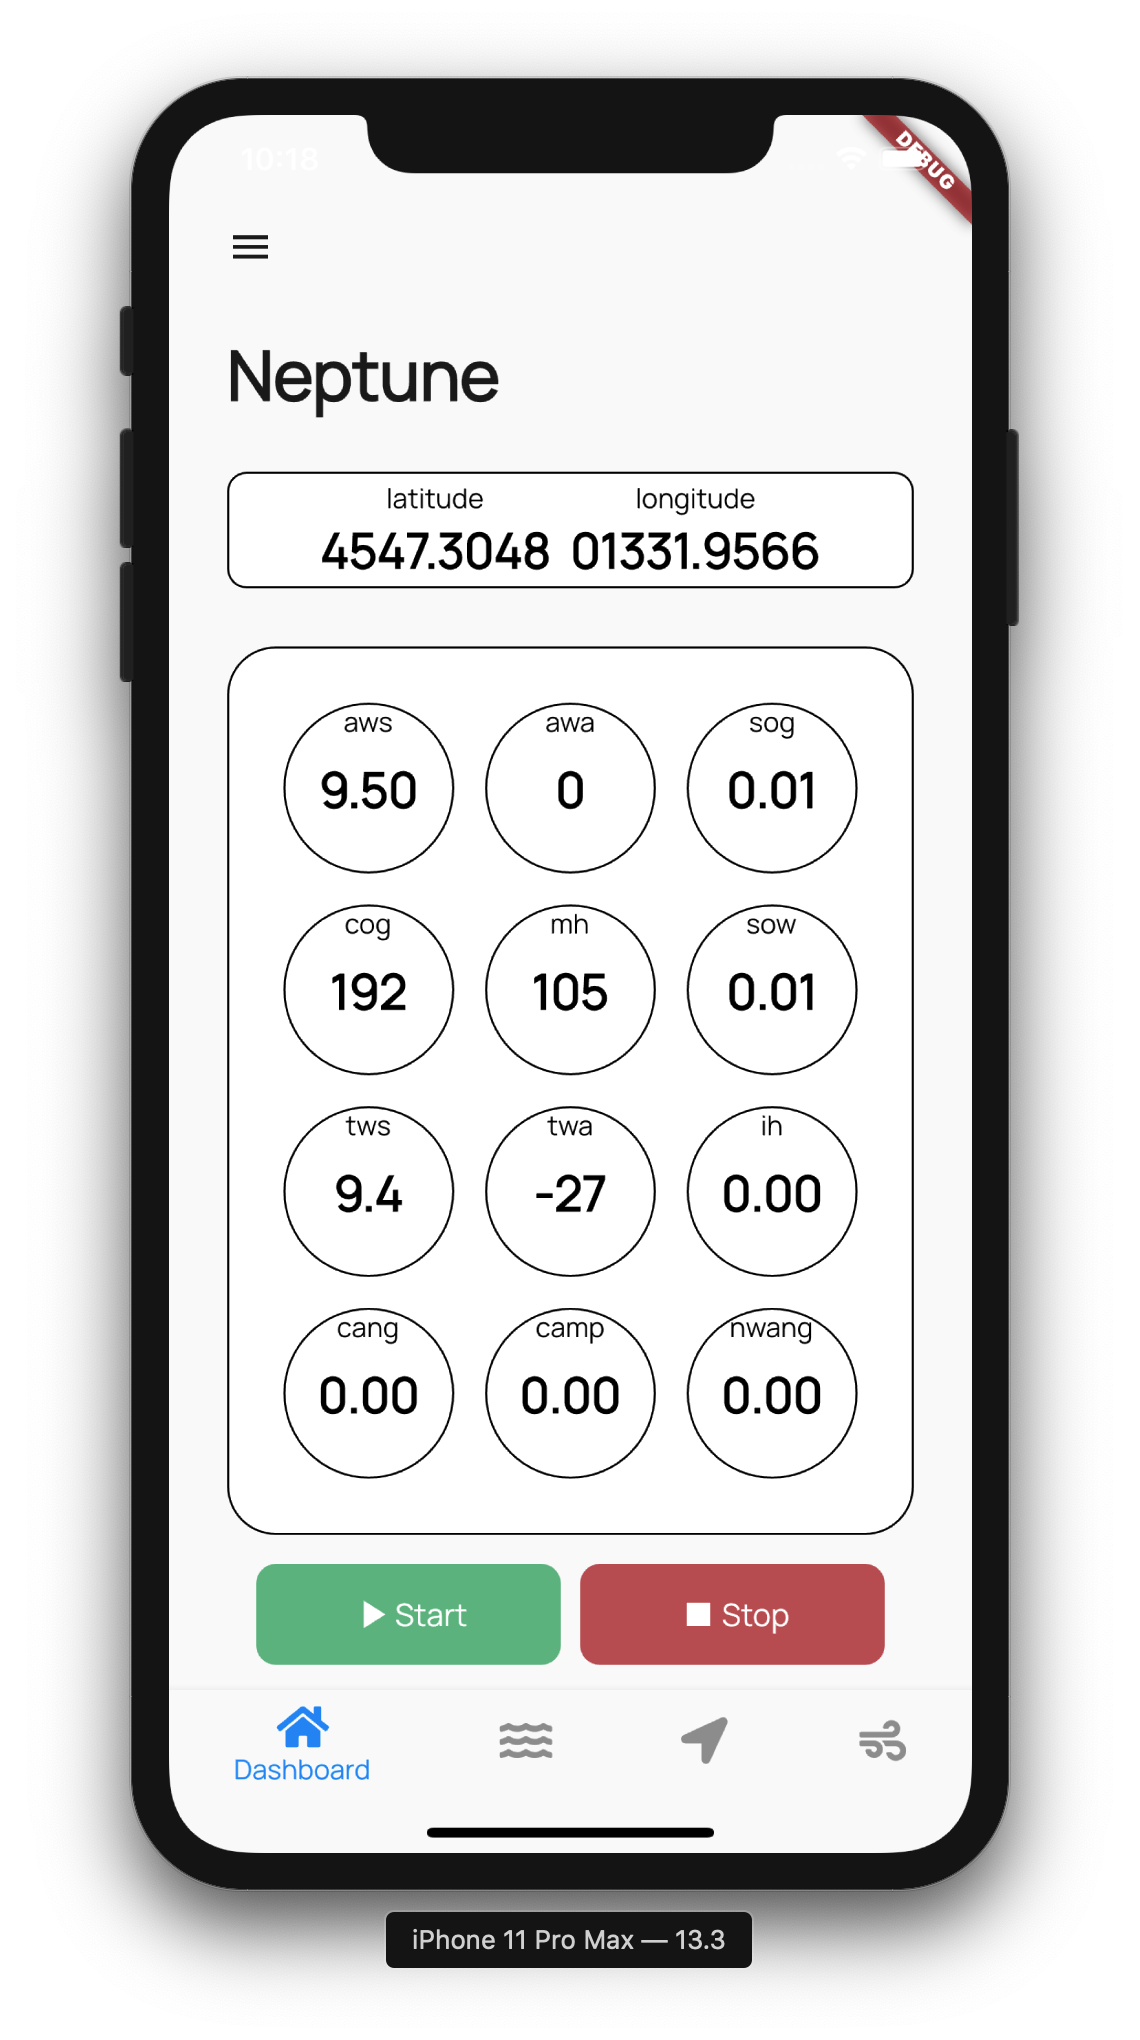
\includegraphics[scale=0.34]{dashboard_high_contrast}
	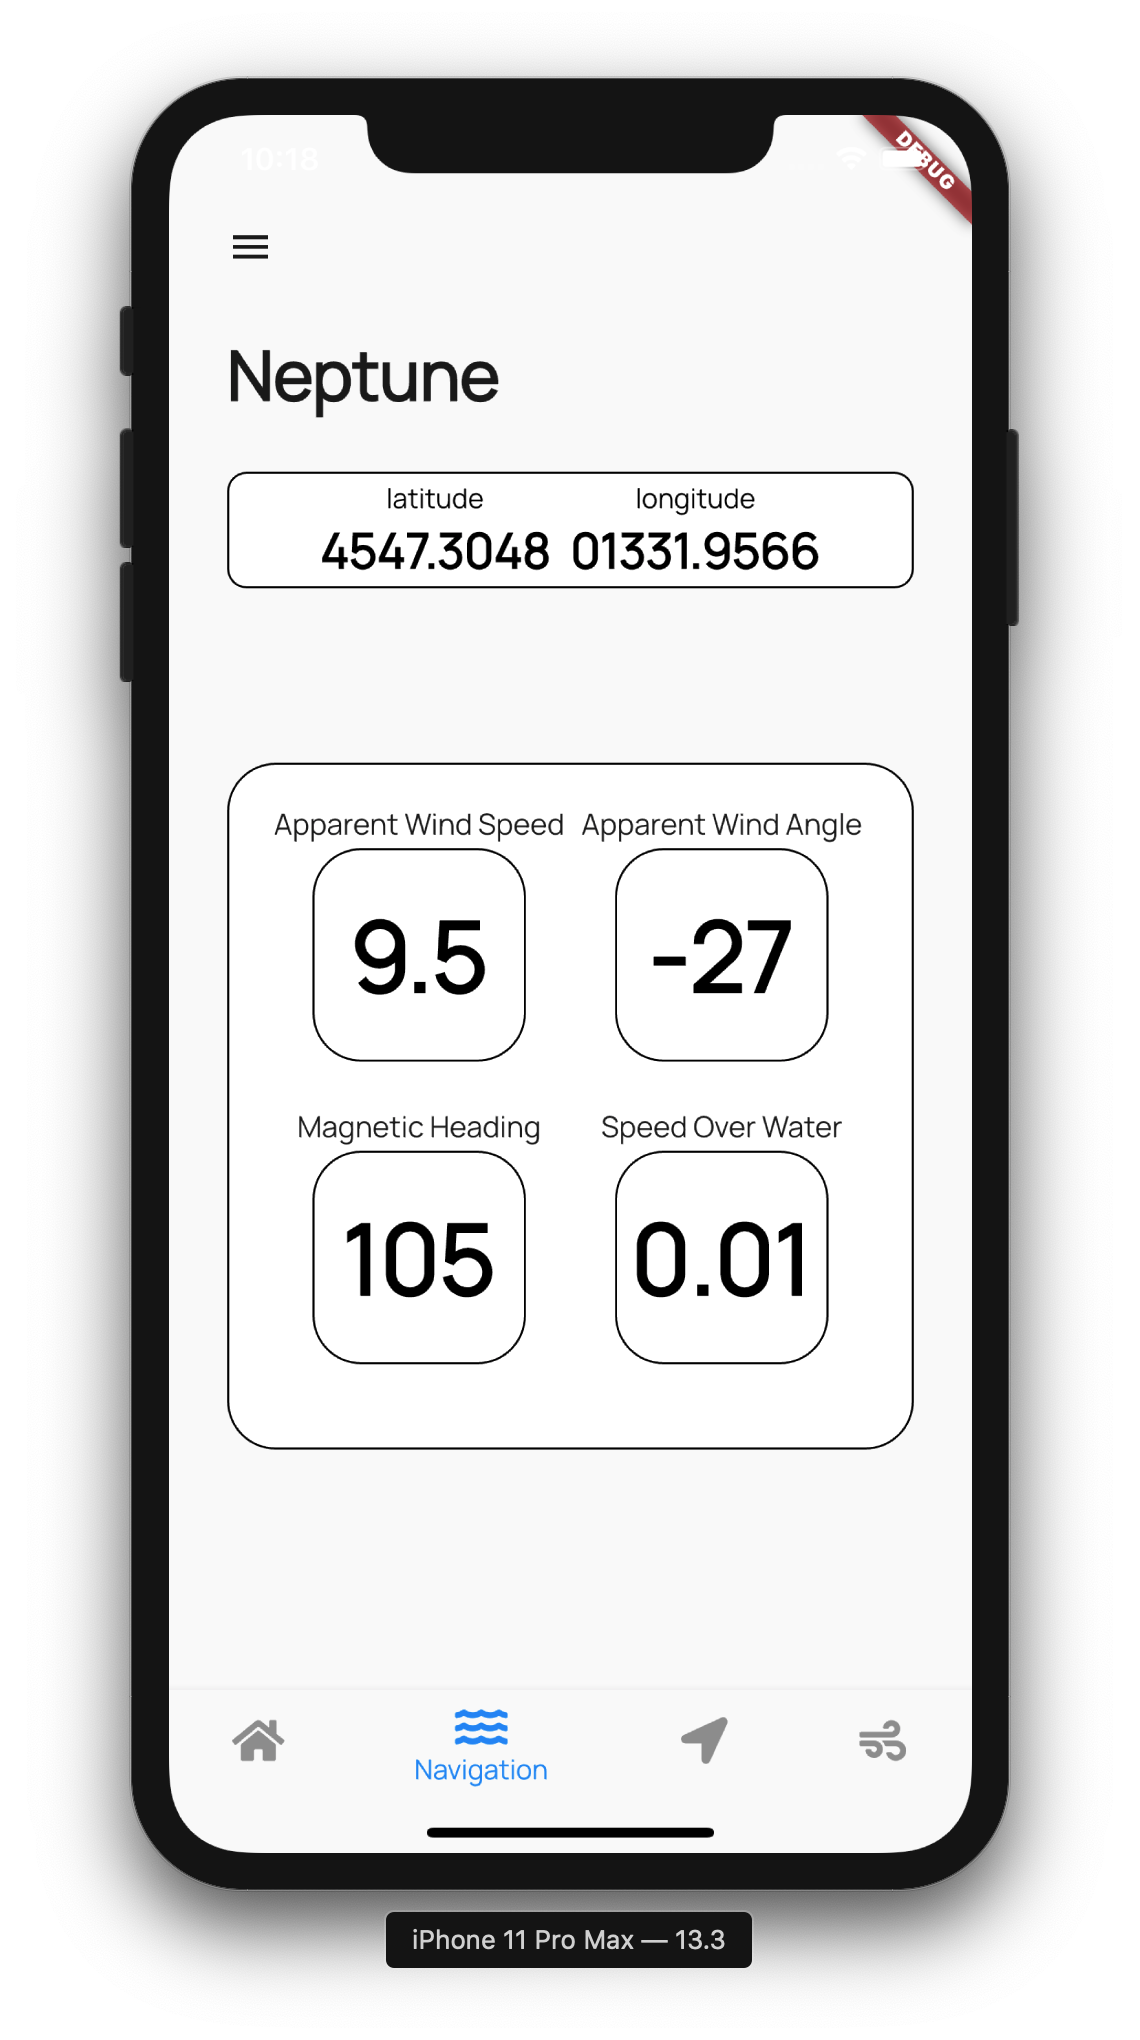
\includegraphics[scale=0.34]{navigation_high_contrast}
	\caption[Screenshot - Dashboard e Navigation con tema ad alto contrasto]{È possibile notare le schermate \textit{Dashboard} e \textit{Navigation} (in ordine da sinistra) con l'applicazione ad \textit{alto contrasto}.}\label{xyz}
\end{figure}

\newpage

\subsection{Widget comuni}
L'interfaccia grafica è stata realizzata utilizzando dei Widget creati \textit{ad-hoc}. Grazie a Flutter e alla flessibilità dell'architettura implementata, questi Widget possono essere aggiunti facilmente in una schermata e risulta molto semplice integrarli, a livello di codice.

\subsubsection{GridBox}
Questo Widget viene utilizzato dalle schermate \textit{Navigation}, \textit{GPS} e \textit{Wind} (Figura 6.19). È un Widget che costruisce una griglia quadrata \verb|2 x 2|, in cui mostrare i dati da monitorare. Gli elementi che compongono la griglia sono stati costruiti per composizione con altri Widget elementari e la loro struttura risulta essere complessa. Tuttavia, la semplicità con cui questo Widget può essere integrato nelle varie schermate rappresenta un grande vantaggio. Tutta la complessità dell'implementazione della griglia è incapsulata all'interno della classe \verb|GridBox|.
Il codice che viene proposto, è stato preso dalla schermata \verb|Navigation|. Dalla riga 11 alla riga 15 è possibile notare la semplicità con cui viene effettuata la chiamata al Widget \verb|GridBox|, passando i relativi parametri, necessari per istanziare correttamente il Widget con dei valori iniziali e per gestire gli aggiornamenti futuri.

\begin{lstlisting}
...

class _NavigationPageState extends State<NavigationPage>
    with AutomaticKeepAliveClientMixin<NavigationPage> {
  @override
  bool get wantKeepAlive => true;

  @override
  Widget build(BuildContext context) {
    super.build(context);
    return GridBox(
      bloc: widget.navigationBloc,
      themeHandler: widget.themeHandler,
      initialData: Navigation(),
    );
  }
}

...
\end{lstlisting}

\begin{figure}
	\begin{center}
		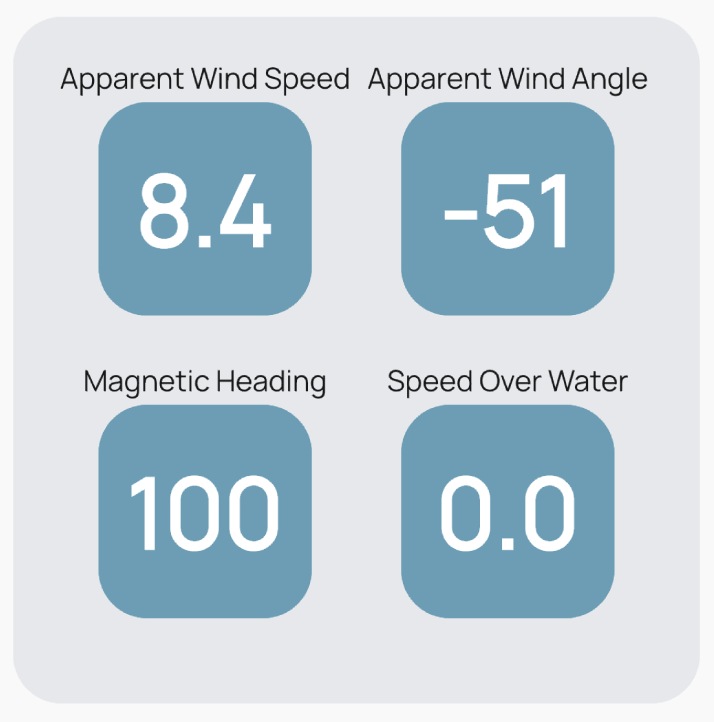
\includegraphics[scale=0.5]{grid_box_widget}
		\caption[Screenshot - GridBox Widget]{Screenshot del Widget \textit{GridBox}. Lo stesso Widget è stato integrato nelle schermate \textit{Navigation}, \textit{GPS} e \textit{Wind}.}
		\label{figura:grid_box_widget}
	\end{center}
\end{figure}

\subsubsection{Location}
\begin{figure}
	\begin{center}
		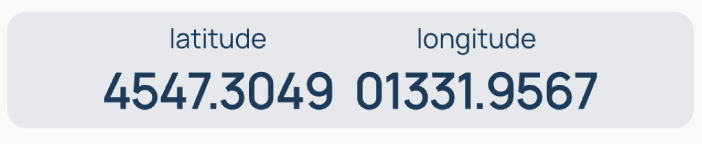
\includegraphics[scale=0.6]{location_widget}
		\caption[Screenshot - Location Widget]{Screenshot del Widget \textit{Location}. Lo stesso Widget è stato integrato in tutte e quattro le schermate.}
		\label{figura:location_widget}
	\end{center}
\end{figure}

Questo Widget permette di visualizzare i dati relativi alla \textit{geolocalizzazione} (Figura 6.20). Il Widget \verb|Location| è presente in tutte le quattro schermate dell'applicazione. È posto nella parte superiore dello schermo, in modo che l'utente possa monitorare continuamente i parametri visualizzati, anche quando passa da una schermata all'altra.

Il codice che verrà illustrato, è stato preso dalla classe \verb|DashboardPage|. Per poter utilizzare questo WIdget bisogna effettuare una chiamata al metodo \verb|create| di \verb|Location| (riga 7). Anche in questo caso, è possibile notare la semplicità con cui i Widget, anche se personalizzati e possiedono una loro logica, possono essere integrati in varie parti dell'applicazione. Infatti, il Widget ha un suo BLoC per interagire con il Repository.

\newpage

\begin{lstlisting}
...
Widget _buildUI() {
    return ListView(
      shrinkWrap: true,
      children: <Widget>[
        LocationWidget.create(context),
        DashboardWidget.create(context),
      ],
    );
  }
...
\end{lstlisting}

\begin{figure}[htp]
	\centering
	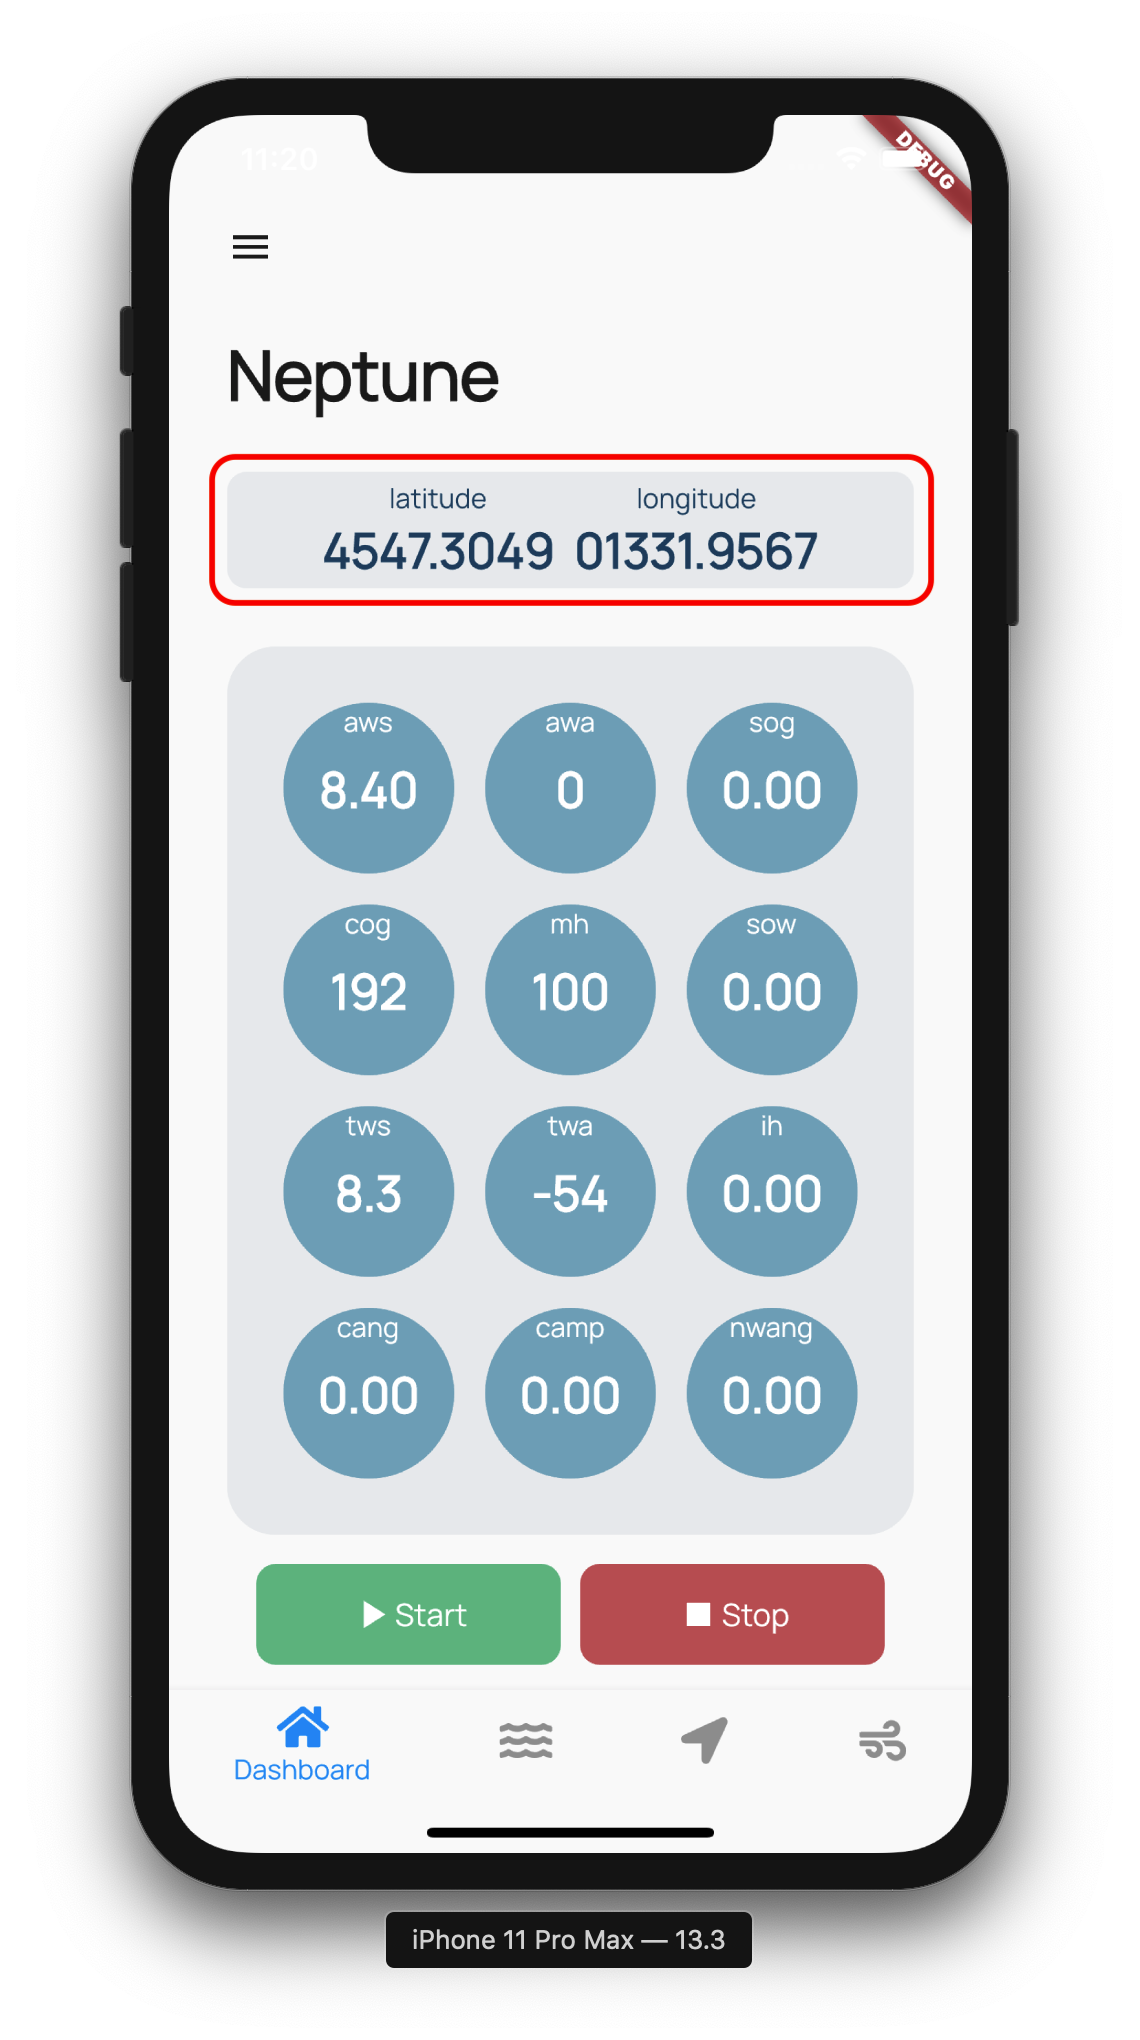
\includegraphics[scale=0.34]{location_widget_dashboard}
	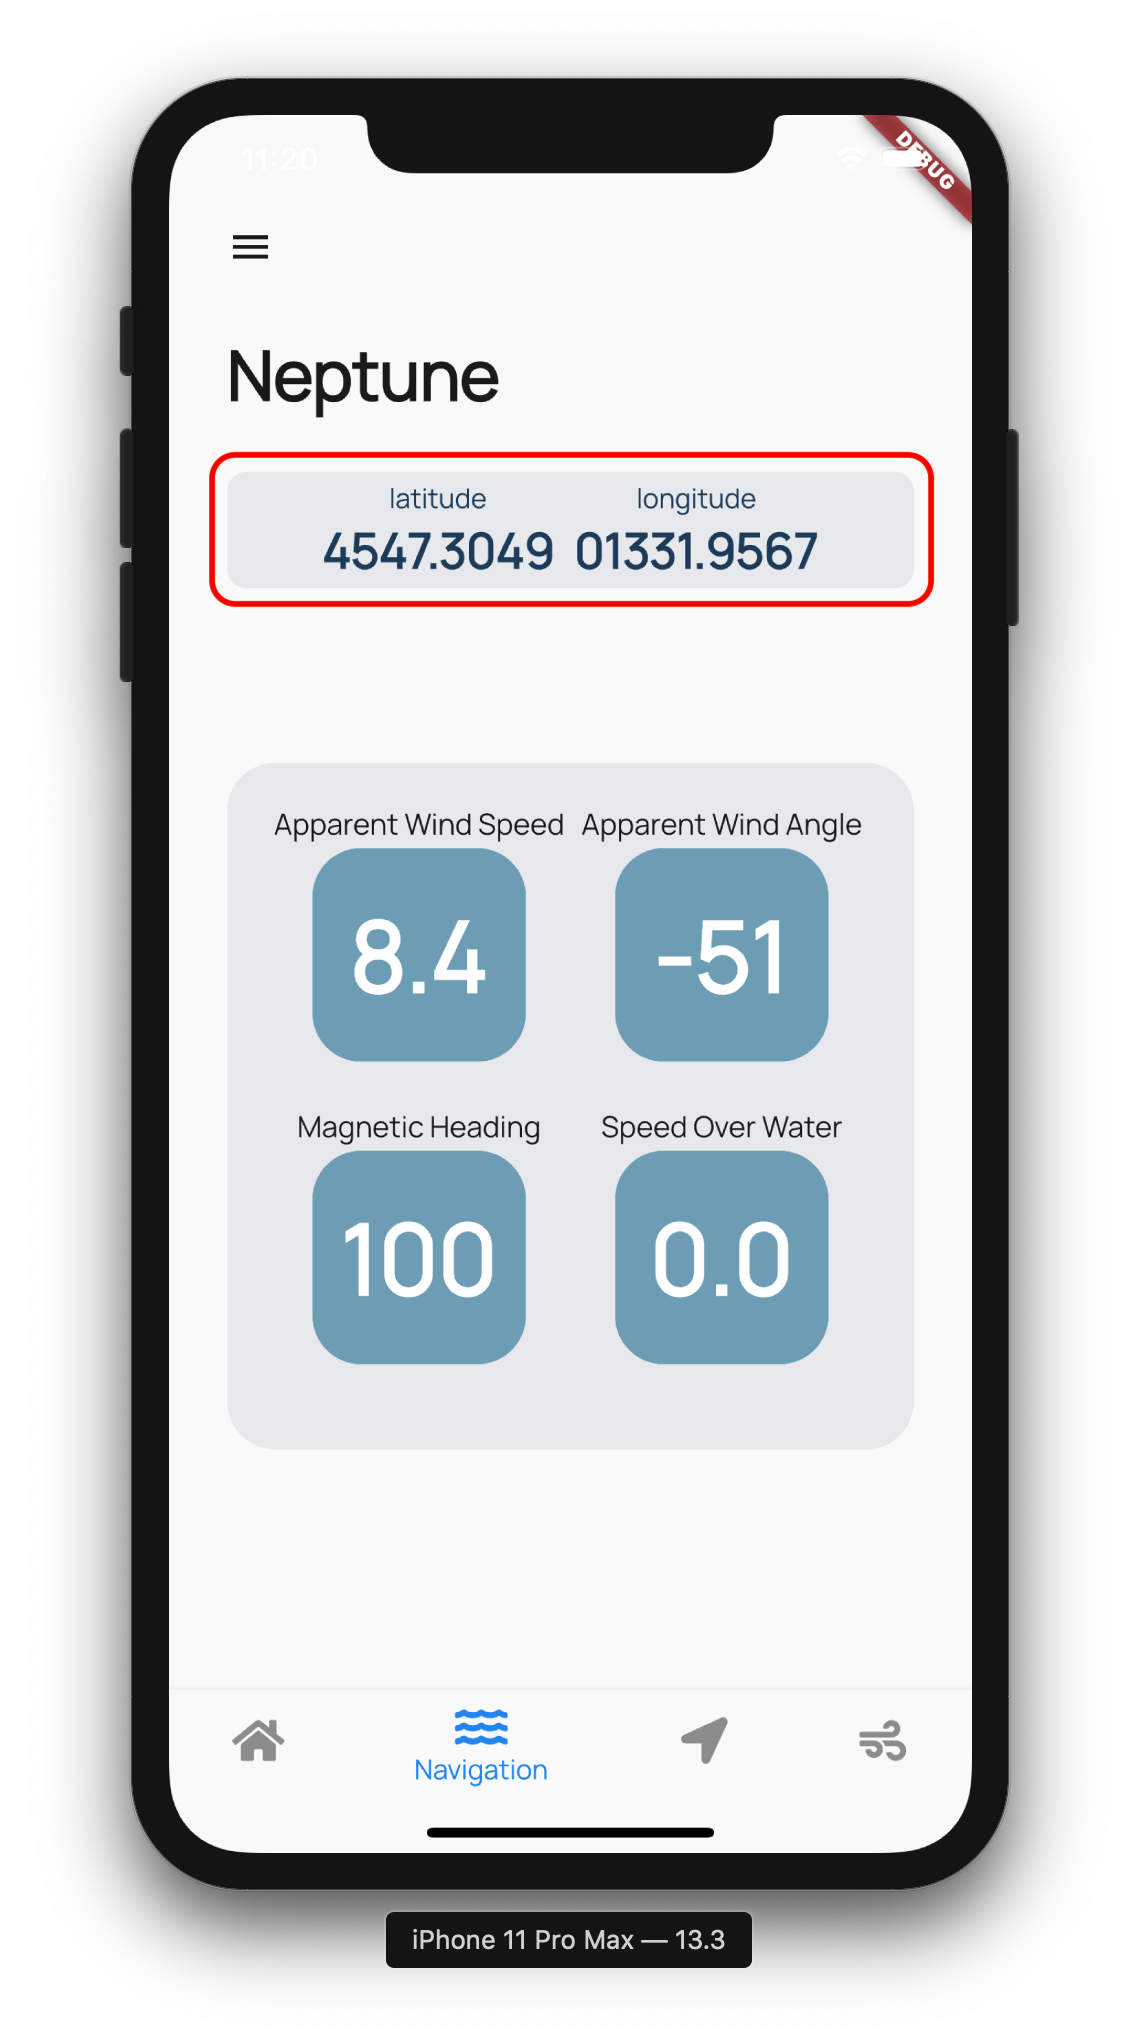
\includegraphics[scale=0.34]{location_widget_navigation}
	\caption[Screenshot - Location Widget nelle schermate Dashboard e Navigation]{Il Widget \textit{Location} nelle schermate \textit{Dashboard} (a sinistra) e \textit{Navigation} (a destra).}\label{xyz}
\end{figure}

\newpage

\subsubsection{Page App Bar}
Questo Widget va a modificare l'\textit{App Bar} di base fornita da Flutter. Questa App Bar viene utilizzata principalmente nelle schermate relative alle impostazioni, quindi nelle schermate \textit{Settings}, \textit{Cache}, \textit{Server} e \textit{Theme}. Lo screen della Figura 6.22 è stato preso dalla schermata \textit{Server}. La flessibilità di questo Widget è data dalla possibilità di modificare il titolo dell'App Bar, in quanto può essere utilizzata, appunto, su molteplici schermate.

\begin{figure}
	\begin{center}
		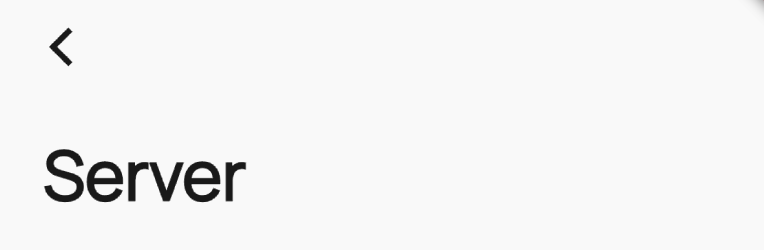
\includegraphics[scale=0.5]{page_app_bar}
		\caption[Screenshot - Page App Bar]{Screenshot del Widget \textit{Page App Bar}. Lo stesso Widget è stato integrato principalmente nelle schermate relative alle impostazioni.}
		\label{figura:page_app_bar}
	\end{center}
\end{figure}

\subsubsection{Sensor Data App Bar}
\verb|Sensor Data App Bar| è un Widget molto simile al precedente (Figura 6.23). Le differenze sostanziali riguardano principalmente gli aspetti grafici. Questo Widget ha la medesima flessibilità del precedente. \verb|Sensor Data App Bar| viene utilizzato nelle schermate dedicate ai dettagli di un dato preciso. Questa funzionalità non è stata implementata, ma ne è stato predisposto l'ambiente.

\begin{figure}
	\begin{center}
		
\includegraphics[scale=0.5]{sensor_data_app_bar}
		\caption[Screenshot - Sensor Data App Bar]{Screenshot del Widget \textit{Sensor Data App Bar}. Lo stesso Widget è stato integrato in tutte le schermate che permettono di visualizzare i dettagli di un particolare dato.}
		\label{figura:sensor_data_app_bar}
	\end{center}
\end{figure}

\newpage

\subsection{Palette di colori}
Questa classe fa parte del \textit{package} \verb|utils| e raccoglie tutti i colori personalizzati che sono stati utilizzati nell'applicazione.

Uno dei principali motivi della realizzazione di quest'applicazione era la creazione di un'interfaccia che potesse presentare i dati in maniera più efficace, rivisitando l'aspetto grafico. Pertanto, l'implementazione di questa classe ha un valore importante all'interno del progetto, nonostante non contenga una complessità paragonabile ad altri elementi dell'app.

Di seguito viene mostrato un breve esempio del contenuto di questa classe.

\begin{lstlisting}
...

// Red
static Color redAccent           = Color.fromRGBO(255, 87, 87, 1);
static Color redBackground   = Color.fromRGBO(198, 35, 38, 0.1);
static Color redButton            = Color.fromRGBO(178, 34, 34, 0.7);

...
\end{lstlisting}

\subsection{Temi}
Questa classe è collocata all'interno del package \verb|utils| e permette di gestire il tema dell'applicazione. L'applicazione ha principalmente due temi: 
\begin{enumerate}
	\item \textbf{\textit{default}}: è il tema che si presenta all'apertura dell'applicazione;
	\item \textbf{\textit{alto contrasto}}: è un tema che utilizza soltanto il bianco ed il nero. Questo tema mette in evidenza gli elementi dell'applicazione sopratutto quando il tempo metereologico è soleggiato.
\end{enumerate}

\subsubsection{Themes}
Questa è una semplice classe \textit{enumerazione} in cui vengono elencati i vari nomi dei temi che supporta l'applicazione. Se in futuro verranno realizzati ulteriori temi, sarà necessario aggiornare questa classe.

\begin{lstlisting}
enum Themes {
  DEFAULT,
  HIGH_CONTRAST
}
\end{lstlisting}

\subsubsection{CustomTheme}
\verb|CustomTheme| è un'\textit{interfaccia} (anche se viene dichiarata come una classe astratta, si veda l'Appendice \ref{cap:A} per ulteriori spiegazioni) che fornisce dei metodi comuni per implementare tutti i temi. Di seguito viene presentato l'elenco dei metodi:
\begin{enumerate}
	\item \verb|Color getBackgroundColorOfSensorData()|
	\item \verb|Color getBorderColorOfSensorData()|
	\item \verb|Color getBackgroundColorOfBox()|
	\item \verb|Color getBackgroundBorderOfBox()|
	\item \verb|Color getTextOfSensorValues()|
	\item \verb|Color getTitleTextOfSensorData()|
	\item \verb|Color getTitleTextOfSensorDataInDashboard()|
	\item \verb|Color getTextColorOfLocation()|
\end{enumerate}
È possibile notare che questi metodi vanno ad operare su delle specifiche componenti grafiche o delle parti di essa. Questa interfaccia può essere ampliata per aumentare la personalizzazione grafica dell'applicazione.

\subsubsection{DefaultTheme e HighContrastTheme}
Queste due classi implementano i metodi dell'interfaccia \verb|CustomTheme|. Ciascuna classe va ad applicare dei specifici colori per realizzare un preciso tema. Il \verb|DefaultTheme| utilizza diversi colori, mentre il \verb|HighContrastTheme| utilizza soltanto i colori bianco e nero.

\subsubsection{ThemeHandler}
Anche questa classe implemente l'interfaccia \verb|CustomTheme|, tuttavia non implementa alcun tema. Questa classe, invece, si occupa di applicare il tema, una volta che è stato scelto dall'utente. Infatti, tramite il metodo \verb|applyTheme| è possibile indicare quale tema si vuole applicare. Il metodo in questione, sulla base del parametro ricevuto, istanzia un oggetto che rappresenta il tema scelto e lo applica all'app. Per poter attuare realmente il cambio di tema, questo metodo deve essere chiamato all'interno del metodo \verb|setState(() {})|, in modo da notificare il framework. Così facendo, il framework rileva un cambiamento di stato dell'applicazione e attua le dovute modifiche al Widget tree, visualizzando il tema scelto dall'utente.

Di seguito si mostra l'implementazione del metodo che permette di applicare il tema.
\begin{lstlisting}
void applyTheme(Themes themeChosen) {
    switch (themeChosen) {
      case Themes.DEFAULT:
        _themeChosen = Themes.DEFAULT;
        theme = DefaultTheme();
        break;
      case Themes.HIGH_CONTRAST:
        _themeChosen = Themes.HIGH_CONTRAST;
        theme = HighContrastTheme();
        break;
    }
  }
\end{lstlisting}

\subsection{Main}
Nel file \verb|main.dart| sono contenute tutte le classi fondamentali per il funzionamento dell'applicazione. La struttura iniziale di questo file viene fornita dal framework stesso nel momento in cui viene creato un nuovo progetto in Flutter.

Con la definizione del metodo \verb|void main() => runApp(MyApp())|, viene fatta eseguire l'applicazione, ovvero, viene avviato tutto il processo di inizializzazione delle varie task e del motore di rendering per visualizzare la grafica.

In questo file viene implementata la struttura essenziale su cui si poggia tutta l'applicazione. In particolare:
\begin{enumerate}
	\item Un \verb|FutureBuilder| che va leggere i dati dal file JSON, salvato nella memoria locale del dispositivo, contenente i dati relativi alla connessione al server e al polling;
	\item Il Provider per la gestione dei \textit{temi} (\verb|Provider<ThemeHandler>|);
	\item \verb|MaterialApp| è un \textit{core} Widget che permette di utilizzare tutti i componenti forniti dal framework. In questo Widget vengono anche definite le caratteristiche basilari dell'applicazione come:
	\begin{enumerate}
		\item Il titolo;
		\item Il colore principale;
		\item Il nome dell'applicazione che verrà visualizzato nel menù delle app del dispositivo;
		\item I Widget che andranno a realizzare l'applicazione nel parametro \verb|home|.
	\end{enumerate}
\end{enumerate}

Vengono definiti inoltre degli altri Widget importanti per la struttura essenziale dell'applicazione, come:
\begin{enumerate}
	\item Un'App Bar personalizzata con il nome dell'applicazione;
	\item Una \verb|BottomNavigationBar| che va a definire una barra di navigazione fissa per tutte le schermate principale, posta nella parte inferiore dell'applicazione. Tramite questo Widget, è possibile navigare da una schermata all'altra tra \textit{Dashboard}, \textit{Navigation}, \textit{GPS} e \textit{Wind};
	\item Un \verb|Drawer|, ovvero, un menù laterale che può essere visualizzato facendo uno \textit{swipe} da sinistra a destra, in cui viene illustrata il logo dell'Università degli Studi di Udine e le opzioni;
	\item Il \verb|body| dell'applicazione in questo caso è una \verb|PageView|. La \verb|PageView| è un Widget che permette di organizzare e di navigare tra le varie schermate, scorrendo a destra e a sinistra. Tramite questo Widget viene offerta un ulteriore modalità per navigare tra le schermate, oltre a quella già fornita dalla \verb|BottomNavigationBar|. Nella \verb|PageView|, vengono effettuate tutte le chiamate alle classi delle principali schermate.
\end{enumerate}

\section{Motivazioni delle scelte grafiche implementate}

\subsection{Concetti generali}
Uno degli obiettivi principali della realizzazione di questa applicazione è la completa rivisitazione dell'interfaccia grafica, cercando di sopperire ai difetti strutturali dell'applicazione Web e dell'applicazione Android. Pertanto, il \textbf{layout} dell'applicazione doveva essere particolarmente curato, in modo da comunicare visivamente all'utente una facile comprensione dell'organizzazione degli elementi. Questo aspetto è di fondamentale importanza, in quanto essendo la \textit{competizione} (la regata) il contesto di applicazione di questo software, è assolutamente necessario che l'utente sia in grado di visualizzare immediatamente i dati di cui necessita. Trovandosi in situazioni in cui si devono svolgere manovre di una certa complessità, la squadra deve concentrarsi nel corretto svolgimento di tali manovre, apportando una minore attenzione all'applicazione. L'applicazione deve aiutare la squadra nel rendere l'attività di monitoraggio dei dati il più semplice e fruibile possibile. L'utente non può impiegare troppo tempo nel capire come funziona l'applicazione o nel capire dove deve andare per poter monitorare un particolare dato: il layout deve essere \textbf{intuitivo}. Se così non fosse, l'utente perderebbe troppo tempo a reperire le giuste informazioni e a capire il suo funzionamento, sprecando così del tempo utile per indirizzare correttamente la barca nel percorso prestabilito. Se invece l'applicazione è intuitiva, la squadra ne trarrà vantaggio, in quanto verrà utilizzata attivamente come supporto alle varie decisioni che vengono prese durante tutta la competizione.

\subsection{Scelte stilistiche attuate}
Per ottenere un'interfaccia grafica pulita e facile da utilizzare, nella maggior parte delle schermate si è fatto uso delle \textit{griglie}. Questo elemento grafico va a disporre gli elementi secondo un certo ordine. Tuttavia, la griglia non va a coprire l'intero schermo del dispositivo, ma va coprire la maggior parte dello spazio dello schermo: sia la griglia che il \textit{Location} Widget sono contenuti all'interno di un box di colore grigio. Il significato è quello di delimitare lo spazio di un determinato elemento, da tutto il resto dell'applicazione. In questo modo l'utente, se deve osservare un determinato dato, sa su quale gruppo di elementi deve andare a porre attenzione.

Inoltre, anche gli \textit{spazi bianchi} tra un elemento e l'altro contribuiscono nell'aspetto e nella percezione del layout. Quando si va a sviluppare un layout, si cerca di ottimizzare tutto lo spazio che si ha a disposizione. Questo è un errore che porta alla realizzazione di un'interfaccia grafica molto complessa e caotica. La presenza di molti elementi che possono cambiare forma o contenuto nel tempo (come nel caso dell'applicazione realizzata), può comportare ad un senso di disorientamento e di confusione all'utente. L'utente può trovare difficoltà nel reperire le informazioni corrette con velocità. Riempire lo schermo di elementi grafici implica un \textbf{sovraccarico cognitivo} da parte dell'utente. Questo fenomeno si verifica quando l'utente riceve troppe informazioni e non è in grado di prendere una decisione o di concentrarsi su un'informazione specifica. Se il layout realizzato presenta queste criticità, è necessario riprogettare interamente l'interfaccia, in quanto l'utilizzo di un'applicazione tale, comporterebbe ad ottenere una pessima \textit{user experience}. Nel contesto in cui viene utilizzata l'app, questo potrebbe esporre la squadra anche a dei pericoli: se l'utente non è in grado di focalizzare la sua attenzione sui dati di cui necessita, l'utente non sarà attento né alle manovre della barca, né ai dati forniti dell'applicazione, che potrebbero avvisarlo, ad esempio, di un qualche malfunzionamento del mezzo.

In conclusione, l'organizzazione degli elementi grafici è stata pensata per la realizzazione di un layout che fosse il più pulito ed ordinato possibile, in modo che l'utente possa andare a reperire velocemente i dati, leggerli e confrontarsi con la squadra sulle decisioni da prendere.

\section{Ottimizzazioni}
In questa sezione, si andranno a descrivere le buone pratiche di programmazione in Flutter e le ottimizzazioni attuate nell'applicazione realizzata, per ottenere dei vantaggi a livello di prestazioni e per offrire all'utente un'interfaccia grafica più fluida e reattiva.

\subsection{Provider e StreamBuilder}
Per ottenere delle migliorie dal punto di vista delle prestazioni, è necessario \textit{abbassare} i Provider e gli StreamBuilder nell'albero dei Widget. Se questi Widget vengono posizionati vicini alla radice, nel momento in cui avviene il cambiamento di stato, tutti i loro sotto-alberi vengono aggiornati dal motore di rendering. Quindi, c'è molta probabilità che in una situazione simile, diversi Widget vengano aggiornati anche quando non lo necessitano, sia perché questi sono \textit{immutabili} o perché semplicemente devono essere aggiornati solo alla ricezioni di determinati dati. Risulta \textit{efficiente} dal punto di vista delle prestazioni, posizionare nel punto più basso possibile questi Widget: così facendo, nel momento in cui vengono ricevuti dei dati, vengono aggiornati soltanto i Widget strettamente essenziali. Questa considerazione può sembrare futile, tuttavia è un tema molto importante da considerare dopo aver sviluppato una prima versione del software. Questa problematica può essere fonte di rallentamenti dell'applicazione, in particolare dell'interfaccia grafica. Di conseguenza l'esperienza utente diventa più difficoltosa e spiacevole.

\subsection{Annidamento degli StreamBuilder}
Un altro aspetto molto importante da considerare nella fase di sviluppo dell'applicazione riguarda l'\textit{annidamento} degli StreamBuilder. Come suggerisce il nome, questi Widget sono direttamente collegati a degli \verb|Stream| e nel momento in cui viene ricevuto un nuovo dato tramite questo flusso, il sotto-albero dello \verb|StreamBuilder| (specificato nel parametro \verb|child|) viene aggiornato dal motore di rendering. Pertanto, annidare più \verb|StreamBuilder| tra loro comporta principalmente a:
\begin{enumerate}
	\item \textbf{Aggiornamenti a cascata}: quando uno \verb|StreamBuilder| riceve un nuovo dato, provoca l'aggiornamento di tutti i Widget sottostanti, compresi gli \verb|StreamBuilder| inclusi nel suo sotto-albero. Così facendo, vengono aggiornati a catena tutti gli \verb|StreamBuilder|, provocando diverse chiamate al motore di rendering. Di conseguenza, l'interfaccia risulterà più lenta e meno reattiva alle interazioni dell'utente e farà uno uso maggiore delle risorse del dispositivo;
	\item \textbf{Aggiornamenti non voluti}: un \textit{effetto collaterale} del punto precedente, è che alcuni Widget vengono forzatamente aggiornati anche quando non lo necessitano. Questa casistica è analoga a quella descritta per i Provider.
\end{enumerate}

\subsection{Ottimizzazioni grafiche}

Per ottenere delle ottimizzazioni delle prestazioni nell'interfaccia grafica, è stato utilizzato il metodo statico \verb|Future.microtask(() { ... })|. Flutter, oltre ad avere un \nameref{Event Loop} (Capitolo 4) in cui inserire tutte le \textit{task} che il framework deve elaborare, ha una seconda coda gestita con politica \textit{FIFO}: \textbf{Microtask Queue}. Questa coda viene dedicata allo svolgimento di quelle task che possono essere elaborate e terminate velocemente. Se delle task vengono inserite in questa coda, il framework va ad eseguire prima queste e poi quelle contenute nella \textit{Event Queue} \cite{future_microtask}.

Nell'applicazione, questo meccanismo è stato utilizzato per velocizzare e rendere più fluida l'apertura delle schermate relative ai dati dei sensori e alle impostazioni. In questo modo, quando l'utente vuole andare a modificare le impostazioni della connessione del server, per esempio, il tap dell'utente viene captato e l'evento viene inserito nella \textit{microtask queue}. Il framework si accorge che in questa coda c'è un evento da elaborare, esegue l'elaborazione e torna a controllare se ci sono degli eventuali eventi nella medesima coda o nelle coda degli eventi. Così facendo, l'apertura delle schermate sarà più reattiva.

Il codice illustrato di seguito, è stato preso dalla classe \verb|GridBox|. Dalla riga 7 alla riga 18 è possibile notare l'utilizzo del metodo \verb|Future.microtask()| per l'apertura di una nuova schermata.

\newpage

\begin{lstlisting}
...

Widget _setupBox(String title, String value) {
    return InkWell(
      onTap: () async {
        Future<Widget> buildPageAsync() async {
          return Future.microtask(() {
            return Scaffold(
              appBar: SensorDataAppBar(context: context, 
              title: title),
              body: Column(
                children: <Widget>[
                  Center(
                    child: _buildBox(title, value),
                  ),
                ],
              ),
            );
          });
        }

        Widget page = await buildPageAsync();
        MaterialPageRoute route = MaterialPageRoute(
        builder: (_) => page);
        Navigator.push(context, route);
      },
      child: _buildBox(title, value),
    );
  }
  
...
\end{lstlisting}

\begin{figure}
	\begin{center}
		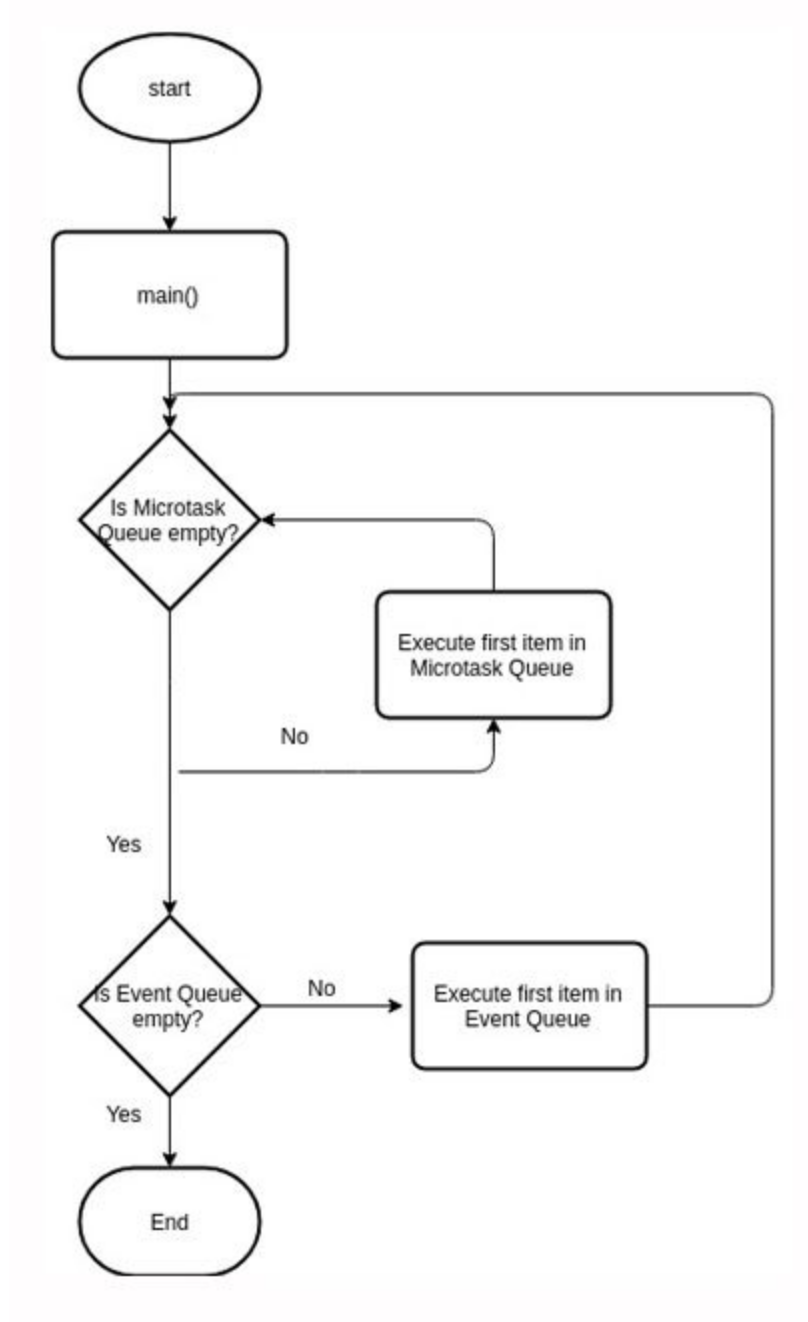
\includegraphics[scale=0.5]{event_queue_microtask_queue}
		\caption[Screenshot - Schema di Event Queue e Microtask Queue]{Uno schema che illustra il funzionamento del meccanismo dell'\textit{Event Queue} e dell'\textit{Microtask Queue}, durante l'esecuzione dell'applicazione \cite{event_queue_microtask_queue}.}
		\label{figura:event_queue_microtask_queue}
	\end{center}
\end{figure}